\documentclass[final,3p,times]{elsarticle}
\usepackage[utf8]{inputenc}
\usepackage{amssymb}
\usepackage{float}
\usepackage{placeins}
\usepackage{amsmath}
\usepackage{booktabs}
\usepackage{textcomp}
\usepackage{multirow}
\usepackage{threeparttable}
\usepackage{siunitx}
\usepackage[table]{xcolor}
\usepackage{xurl}
\usepackage{hyperref}
\usepackage{pgfplots}
\usepgfplotslibrary{colormaps,groupplots,statistics}
\pgfplotsset{compat=1.18}
\usepackage{tikz}
\usetikzlibrary{shapes,arrows.meta,positioning,fit,backgrounds,calc}
\setlength{\marginparwidth}{2cm}
\usepackage{todonotes}
\usepackage{alltt}
\graphicspath{{./}{Images/}}
% --- Inline figure definitions (formerly figures.tex) ---
\setlength{\textfloatsep}{10pt plus 2pt minus 4pt}   % Distance between top/bottom float and text
\setlength{\floatsep}{8pt plus 2pt minus 2pt}       % Distance between two floats
\setlength{\intextsep}{10pt plus 2pt minus 2pt}     % Distance between inline float and text
\renewcommand{\floatpagefraction}{0.7}
\renewcommand{\textfraction}{0.15}
\renewcommand{\topfraction}{0.85}
\renewcommand{\bottomfraction}{0.65}

\newcommand{\plotCriterionMAEByModel}{%
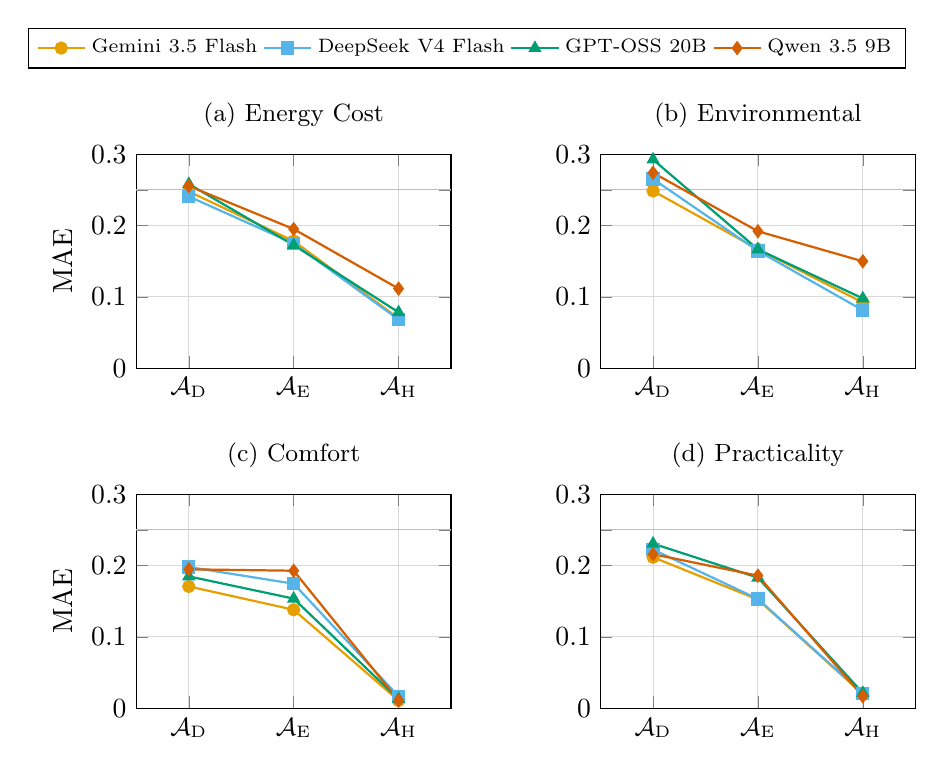
\begin{tikzpicture}
\begin{groupplot}[
    group style={group size=2 by 2, horizontal sep=1.9cm, vertical sep=1.6cm},
    width=0.46\textwidth, height=4.3cm,
    xtick={1,2,3}, xticklabels={$\mathcal{A}_{\text{D}}$,$\mathcal{A}_{\text{E}}$,$\mathcal{A}_{\text{H}}$},
    xticklabel style={font=\small},
    enlarge x limits=0.25,
    grid=major, grid style={gray!30}, ymajorgrids=true,
    extra y ticks={0.25,0.5,0.75},
    extra y tick style={grid=major, grid style={gray!50}},
    extra y tick labels={},
    legend style={font=\scriptsize, at={(1.05,1.4)}, anchor=south, legend columns=4},
    legend cell align={left},
    every axis plot/.append style={thick, mark size=2pt},
]
\nextgroupplot[ylabel={MAE}, ymin=0, ymax=0.3,
    title={\small (a) Energy Cost}, title style={font=\small}]
\addplot[mark=*, colorGemini]   coordinates {(1,0.2477) (2,0.1782) (3,0.0698)};
\addplot[mark=square*, colorDeepSeek] coordinates {(1,0.2407) (2,0.1748) (3,0.0683)};
\addplot[mark=triangle*, colorGPTOSS] coordinates {(1,0.2581) (2,0.1725) (3,0.0783)};
\addplot[mark=diamond*, colorQwen] coordinates {(1,0.2554) (2,0.1950) (3,0.1115)};
\legend{Gemini 3.5 Flash, DeepSeek V4 Flash, GPT-OSS 20B, Qwen 3.5 9B}
\nextgroupplot[ylabel={}, ymin=0, ymax=0.3,
    title={\small (b) Environmental}, title style={font=\small}]
\addplot[mark=*, colorGemini]   coordinates {(1,0.2484) (2,0.1667) (3,0.0921)};
\addplot[mark=square*, colorDeepSeek] coordinates {(1,0.2652) (2,0.1644) (3,0.0812)};
\addplot[mark=triangle*, colorGPTOSS] coordinates {(1,0.2924) (2,0.1665) (3,0.0978)};
\addplot[mark=diamond*, colorQwen] coordinates {(1,0.2739) (2,0.1919) (3,0.1498)};
\nextgroupplot[ylabel={MAE}, ymin=0, ymax=0.3,
    title={\small (c) Comfort}, title style={font=\small}]
\addplot[mark=*, colorGemini]   coordinates {(1,0.1707) (2,0.1380) (3,0.0108)};
\addplot[mark=square*, colorDeepSeek] coordinates {(1,0.1979) (2,0.1745) (3,0.0167)};
\addplot[mark=triangle*, colorGPTOSS] coordinates {(1,0.1848) (2,0.1536) (3,0.0127)};
\addplot[mark=diamond*, colorQwen] coordinates {(1,0.1947) (2,0.1927) (3,0.0108)};
\nextgroupplot[ylabel={}, ymin=0, ymax=0.3,
    title={\small (d) Practicality}, title style={font=\small}]
\addplot[mark=*, colorGemini]   coordinates {(1,0.2116) (2,0.1523) (3,0.0197)};
\addplot[mark=square*, colorDeepSeek] coordinates {(1,0.2224) (2,0.1531) (3,0.0208)};
\addplot[mark=triangle*, colorGPTOSS] coordinates {(1,0.2307) (2,0.1830) (3,0.0213)};
\addplot[mark=diamond*, colorQwen] coordinates {(1,0.2159) (2,0.1858) (3,0.0168)};
\end{groupplot}
\end{tikzpicture}%
}

\newcommand{\plotDecisionTypeByModel}{%
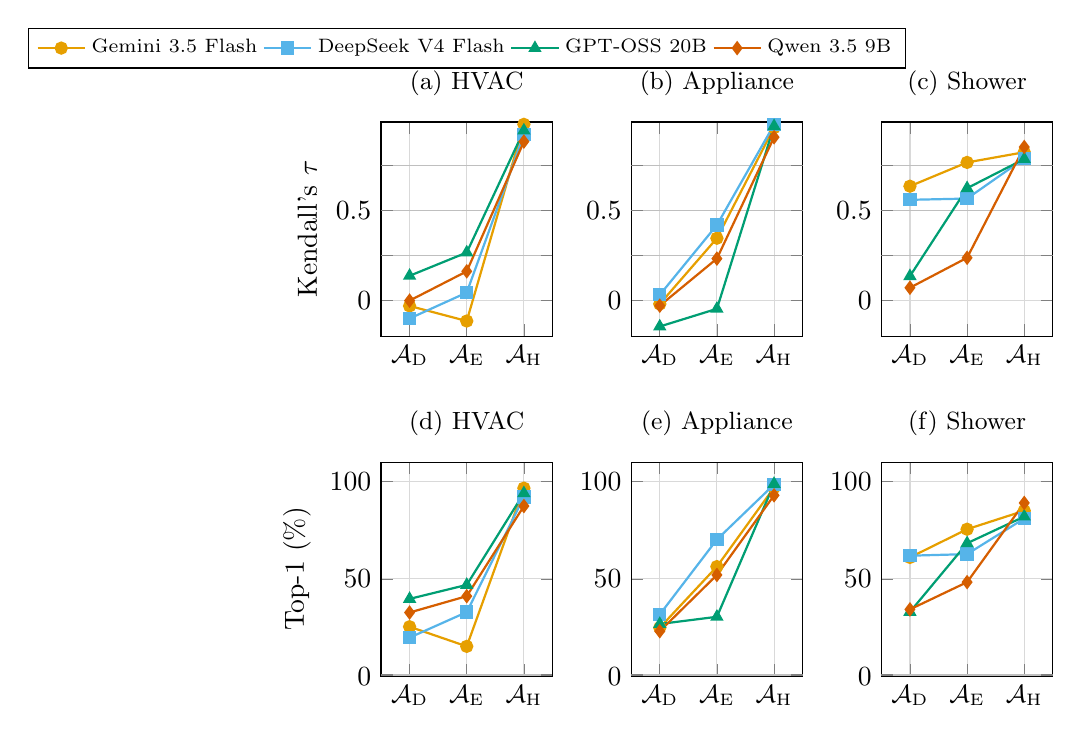
\begin{tikzpicture}
\begin{groupplot}[
    group style={group size=3 by 2, vertical sep=1.6cm},
    width=0.31\textwidth, height=4.3cm,
    xtick={1,2,3}, xticklabels={$\mathcal{A}_{\text{D}}$,$\mathcal{A}_{\text{E}}$,$\mathcal{A}_{\text{H}}$},
    xticklabel style={font=\small},
    enlarge x limits=0.25,
    grid=major, grid style={gray!30}, ymajorgrids=true,
    extra y ticks={0.25,0.5,0.75},
    extra y tick style={grid=major, grid style={gray!50}},
    extra y tick labels={},
    legend style={font=\scriptsize, at={(0.5,1.25)}, anchor=south, legend columns=4},
    legend cell align={left},
    every axis plot/.append style={thick, mark size=2pt},
]
\nextgroupplot[ylabel={Kendall's $\tau$}, ymin=-0.2, ymax=0.99,
    title={\small (a) HVAC}, title style={font=\small}]
\addplot[mark=*, colorGemini]   coordinates {(1,-0.0324) (2,-0.1162) (3,0.9772)};
\addplot[mark=square*, colorDeepSeek] coordinates {(1,-0.1021) (2,0.0419) (3,0.9197)};
\addplot[mark=triangle*, colorGPTOSS] coordinates {(1,0.1352) (2,0.2647) (3,0.9428)};
\addplot[mark=diamond*, colorQwen] coordinates {(1,-0.0027) (2,0.1600) (3,0.8813)};
\legend{Gemini 3.5 Flash, DeepSeek V4 Flash, GPT-OSS 20B, Qwen 3.5 9B}
\nextgroupplot[ylabel={}, ymin=-0.2, ymax=0.99,
    title={\small (b) Appliance}, title style={font=\small}]
\addplot[mark=*, colorGemini]   coordinates {(1,-0.0215) (2,0.3441) (3,0.9590)};
\addplot[mark=square*, colorDeepSeek] coordinates {(1,0.0293) (2,0.4174) (3,0.9754)};
\addplot[mark=triangle*, colorGPTOSS] coordinates {(1,-0.1467) (2,-0.0482) (3,0.9672)};
\addplot[mark=diamond*, colorQwen] coordinates {(1,-0.0309) (2,0.2308) (3,0.9056)};
\nextgroupplot[ylabel={}, ymin=-0.2, ymax=0.99,
    title={\small (c) Shower}, title style={font=\small}]
\addplot[mark=*, colorGemini]   coordinates {(1,0.6333) (2,0.7655) (3,0.8222)};
\addplot[mark=square*, colorDeepSeek] coordinates {(1,0.5576) (2,0.5645) (3,0.7867)};
\addplot[mark=triangle*, colorGPTOSS] coordinates {(1,0.1333) (2,0.6222) (3,0.7845)};
\addplot[mark=diamond*, colorQwen] coordinates {(1,0.0689) (2,0.2355) (3,0.8511)};
\nextgroupplot[ylabel={Top-1 (\%)}, ymin=0, ymax=110,
    title={\small (d) HVAC}, title style={font=\small}]
\addplot[mark=*, colorGemini]   coordinates {(1,25.4) (2,15.3) (3,96.6)};
\addplot[mark=square*, colorDeepSeek] coordinates {(1,19.8) (2,32.9) (3,92.0)};
\addplot[mark=triangle*, colorGPTOSS] coordinates {(1,39.7) (2,46.9) (3,94.0)};
\addplot[mark=diamond*, colorQwen] coordinates {(1,32.7) (2,41.1) (3,87.4)};
\nextgroupplot[ylabel={}, ymin=0, ymax=110,
    title={\small (e) Appliance}, title style={font=\small}]
\addplot[mark=*, colorGemini]   coordinates {(1,24.9) (2,56.3) (3,96.9)};
\addplot[mark=square*, colorDeepSeek] coordinates {(1,31.7) (2,70.2) (3,98.5)};
\addplot[mark=triangle*, colorGPTOSS] coordinates {(1,26.8) (2,30.5) (3,98.8)};
\addplot[mark=diamond*, colorQwen] coordinates {(1,23.1) (2,52.0) (3,92.9)};
\nextgroupplot[ylabel={}, ymin=0, ymax=110,
    title={\small (f) Shower}, title style={font=\small}]
\addplot[mark=*, colorGemini]   coordinates {(1,61.0) (2,75.5) (3,85.0)};
\addplot[mark=square*, colorDeepSeek] coordinates {(1,61.9) (2,62.7) (3,81.0)};
\addplot[mark=triangle*, colorGPTOSS] coordinates {(1,33.0) (2,68.3) (3,82.0)};
\addplot[mark=diamond*, colorQwen] coordinates {(1,34.3) (2,48.3) (3,89.0)};
\end{groupplot}
\end{tikzpicture}%
}

\newcommand{\plotRagAblation}{%
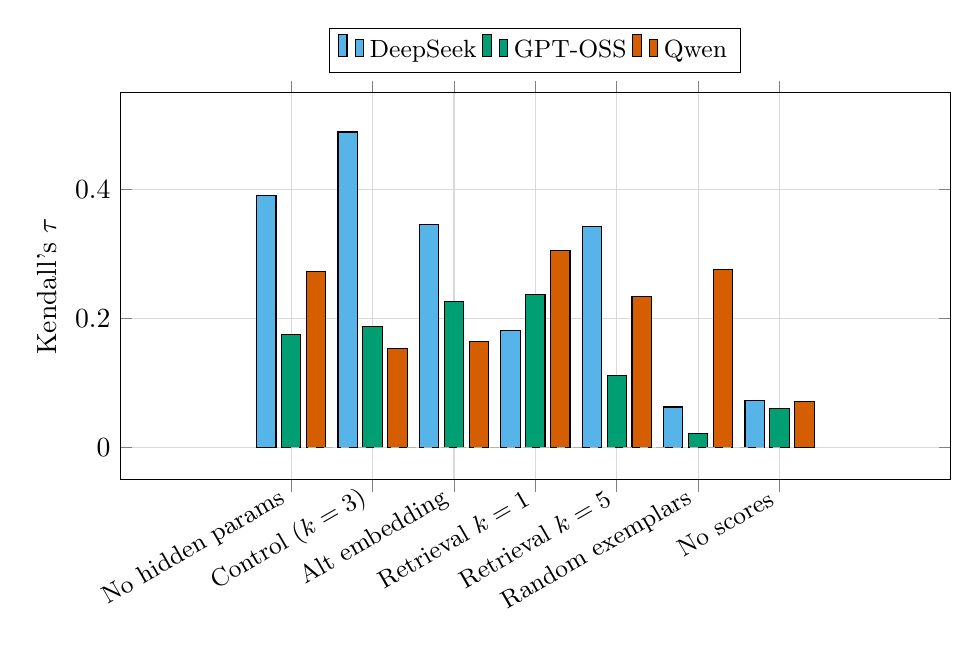
\begin{tikzpicture}
\begin{axis}[
    width=\textwidth, height=6.5cm,
    ylabel={Kendall's $\tau$},
    symbolic x coords={No hidden params,Control ($k=3$),Alt embedding,Retrieval $k=1$,Retrieval $k=5$,Random exemplars,No scores},
    xtick=data,
    xticklabel style={rotate=30, anchor=east, font=\small, align=center},
    enlarge x limits=0.35,
    bar width=7pt,
    ybar,
    ymin=-0.05, ymax=0.55,
    legend style={font=\small, at={(0.5,1.05)}, anchor=south, legend columns=3},
    legend cell align={left},
    grid=major,
    grid style={gray!30},
    ymajorgrids=true,
]
\addplot[fill=colorDeepSeek] coordinates {
    (No hidden params,0.391)
    (Control ($k=3$),0.489)
    (Alt embedding,0.346)
    (Retrieval $k=1$,0.182)
    (Retrieval $k=5$,0.342)
    (Random exemplars,0.063)
    (No scores,0.073)
};
\addplot[fill=colorGPTOSS] coordinates {
    (No hidden params,0.175)
    (Control ($k=3$),0.187)
    (Alt embedding,0.227)
    (Retrieval $k=1$,0.237)
    (Retrieval $k=5$,0.112)
    (Random exemplars,0.022)
    (No scores,0.061)
};
\addplot[fill=colorQwen] coordinates {
    (No hidden params,0.273)
    (Control ($k=3$),0.154)
    (Alt embedding,0.165)
    (Retrieval $k=1$,0.306)
    (Retrieval $k=5$,0.234)
    (Random exemplars,0.276)
    (No scores,0.071)
};
\addplot[dashed, gray!60, sharp plot, update limits=false] coordinates {
    (No hidden params,0) (No scores,0)
};
\legend{DeepSeek,GPT-OSS,Qwen}
\end{axis}
\end{tikzpicture}%
}

\newcommand{\plotSensitivityTau}{%
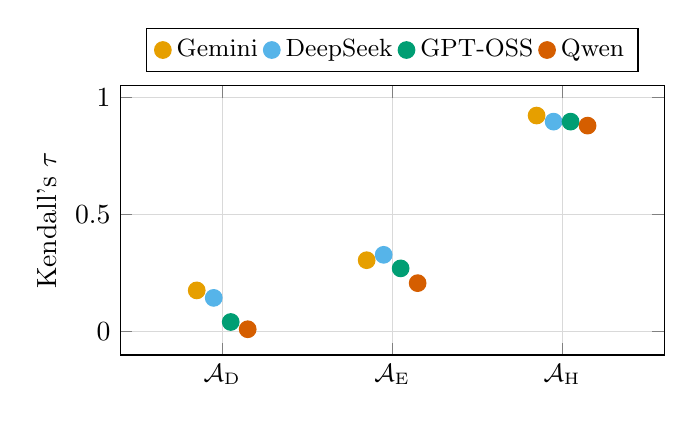
\begin{tikzpicture}
\begin{axis}[
    width=0.7\textwidth, height=5cm,
    ylabel={Kendall's $\tau$},
    xtick={1,2,3},
    xticklabels={$\mathcal{A}_{\text{D}}$,$\mathcal{A}_{\text{E}}$,$\mathcal{A}_{\text{H}}$},
    xticklabel style={font=\small},
    xmin=0.4, xmax=3.6,
    ymin=-0.1, ymax=1.05,
    grid=major,
    grid style={gray!30},
    ymajorgrids=true,
    legend style={font=\small, at={(0.5,1.05)}, anchor=south, legend columns=4},
    legend cell align={left},
]
\addplot[only marks, mark=*, mark size=3pt, color=colorGemini] coordinates {
    (0.85, 0.176) (1.85, 0.305) (2.85, 0.923)
};
\addplot[only marks, mark=*, mark size=3pt, color=colorDeepSeek] coordinates {
    (0.95, 0.144) (1.95, 0.328) (2.95, 0.897)
};
\addplot[only marks, mark=*, mark size=3pt, color=colorGPTOSS] coordinates {
    (1.05, 0.041) (2.05, 0.270) (3.05, 0.897)
};
\addplot[only marks, mark=*, mark size=3pt, color=colorQwen] coordinates {
    (1.15, 0.010) (2.15, 0.207) (3.15, 0.880)
};
\legend{Gemini, DeepSeek, GPT-OSS, Qwen}
\end{axis}
\end{tikzpicture}%
}

% --- End inline figure definitions ---
\definecolor{colorPure}{RGB}{180,180,180}
\definecolor{colorRAG}{RGB}{100,149,200}
\definecolor{colorLLMParameterizedReferenceScoring}{RGB}{31,73,125}
\definecolor{colorGemini}{HTML}{E69F00}
\definecolor{colorDeepSeek}{HTML}{56B4E9}
\definecolor{colorGPTOSS}{HTML}{009E73}
\definecolor{colorQwen}{HTML}{D55E00}
\journal{Environmental Modelling \& Software}
\begin{document}
\begin{frontmatter}
\title{Benchmarking LLM Integration Strategies for MCDA-Assisted Household Energy Decision Support}
\author{Ahaan Nigam\corref{cor1}}
\cortext[cor1]{Corresponding author.}
\ead{ishaannigam27@gmail.com}
\affiliation{organization={Downingtown East High School},
            city={Exton},
            state={Pennsylvania},
            country={USA}}
\author{River Huang}
\affiliation{organization={Paul Scherrer Institut},
            city={Villigen},
            state={Aargau},
            country={Switzerland}}
\begin{abstract}
The residential sector is a major source of global CO\textsubscript{2} emissions, yet most households rely on biased decisions rather than tailored ones. Multi-Attribute Value Theory (MAVT) offers a rigorous Multi-Criteria Decision Analysis (MCDA) method to reduce emissions, but building MCDAs requires expertise that limits household adoption. This study evaluated whether LLMs can bridge that gap by comparing three architectures: Direct LLM Scoring ($\mathcal{A}_{\text{D}}$~), Example-Guided LLM Scoring ($\mathcal{A}_{\text{E}}$~), and LLM-Parameterized Reference Scoring ($\mathcal{A}_{\text{H}}$~), which extracts engineering parameters for a deterministic reference calculator. Reference calculators benchmarked MAVT scores across HVAC, appliance, and shower decisions. $\mathcal{A}_{\text{H}}$ achieved a Kendall's tau of 0.899 and 91.3\% Top-1 accuracy across 195 scenarios; $\mathcal{A}_{\text{E}}$ scored 0.277 and 49.2\%, and $\mathcal{A}_{\text{D}}$ 0.093 and 34.1\%. $\mathcal{A}_{\text{H}}$ also compressed model capability: its tau spanned 0.043 across a 45$\times$ range of model cost, against 0.166 for $\mathcal{A}_{\text{D}}$. Accuracy means agreement with a deterministic reference calculator, not measured household energy data.\end{abstract}
\begin{keyword}
Large language models \sep Multi-criteria decision analysis \sep Multi-Attribute Value Theory \sep Household energy \sep Decision support systems \sep Retrieval-Augmented Generation \sep Sustainability
\end{keyword}
\end{frontmatter}

\section{Introduction}
\label{sec1}
The average U.S.\ household emits roughly 8{,}744 pounds of CO\textsubscript{2}e and consumes about 10{,}791 kWh of electricity each year \cite{epa_household2024,eia_faq_electricity2024}. Globally, residential energy consumption has grown at roughly 1\% per year since 2000, driven by increasing household sizes and comfort demands in emerging economies \cite{GONZALEZTORRES2022112428}. However, a considerable portion of this usage is adjustable, creating opportunities to reduce both household cost and environmental impact \cite{dietz2009,ohler2020}.

Tools that combine optimization, behavioral insight, and decision support can close part of that gap, but only if they are usable without specialized training. Certain frameworks, such as Multi-Criteria Decision Analysis (MCDA), can be used to choose an optimal balance of factors that matter to users \cite{huang2011}. In theory, they would allow environmentally optimal choices consistently accross fields. However, constructing an MCDA model requires defining alternatives, criteria, weights, value functions, and normalization rules, making it impractical for routine household decisions.

It has been proposed in the past that LLMs could be used to automate this process, thus making it practical for household decisions. Without knowing how accurate these LLMs are as experts, it is unclear whether this would be a beneficial or detrimental idea.

Modern LLMs carry general knowledge about the energy use and carbon intensity of common products and behaviours, and many systems can retrieve additional information at inference time. They have not, however, been tested extensively for their abilities as MCDA designers \cite{svoboda2024,icaart26}. It is reasonable to say that they are not consistent decision makers \cite{wang2024fairescalers,li2026scoringbias}. Still, the amount of assistance needed to improve their designer ability to a reasonably accurate level has not been tested either. This study addresses that gap by benchmarking the three architectures across three household energy decision types, holding the model and the MAVT weighting constant for each architecture.

Thus, we aimed to answer the following questions: Which LLM-assisted architecture most accurately reproduces a ground truth produced ranking for rapid household decision support?
Then, how consistently does the architecture ranking hold across models of varying capability?

\section{Literature Review}
\label{sec:lit-review}

\subsection{Household Energy Decision-Making and Adoption Barriers}

Globally, residential buildings account for 18\% of CO\textsubscript{2} emissions \cite{GONZALEZTORRES2022112428}; in the United States, the residential sector consumed 11.8 quadrillion BTU (3{,}458 TWh) of delivered energy in 2022 and accounted for roughly 20\% of national energy-related CO\textsubscript{2} emissions \cite{eia2022,goldstein2020}. If the U.S.\ residential sector were a country, its emissions would rank sixth globally, comparable to Brazil and larger than Germany \cite{goldstein2020}.

Dietz et al.\ (2009) estimated that household behavioral changes could reduce U.S.\ emissions by approximately 451 MtCO\textsubscript{2}e annually, savings that remain available to the average household today \cite{dietz2009}. That potential concentrates in a few areas: HVAC systems alone account for roughly a third of global residential energy consumption \cite{GONZALEZTORRES2022112428}. 

\begin{figure}[H]
	\centering
	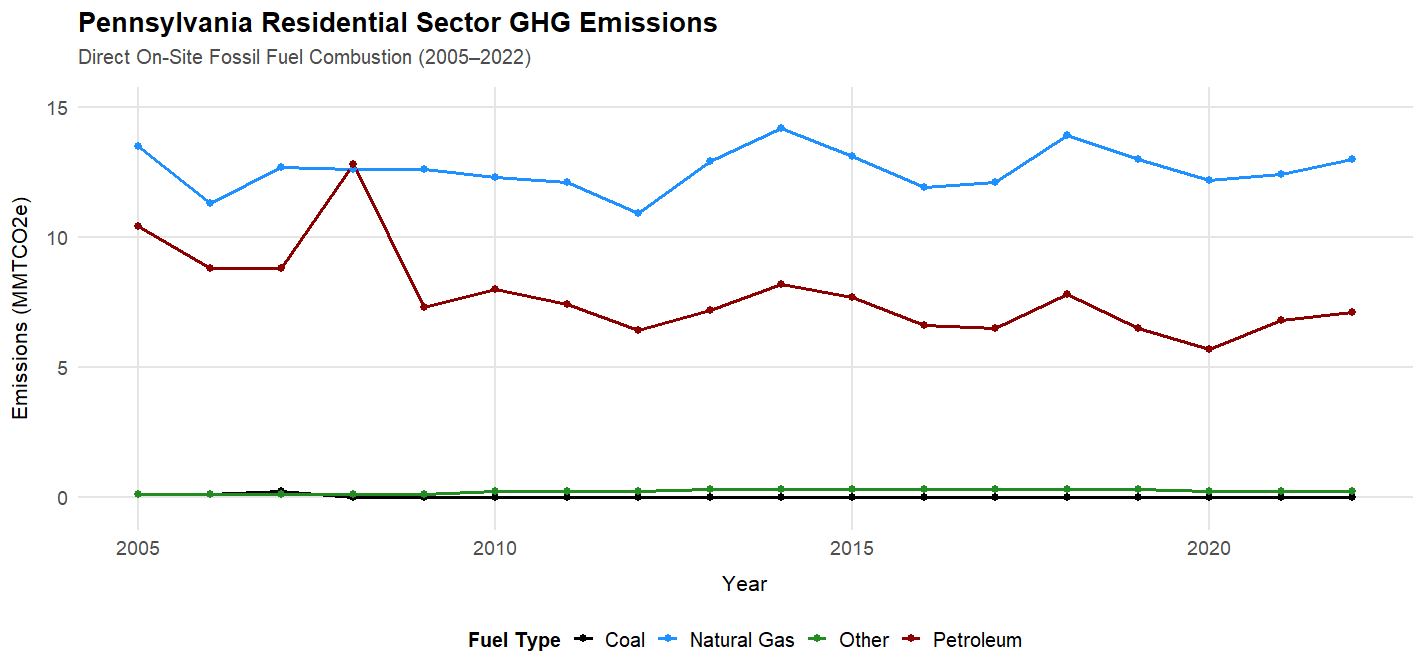
\includegraphics[width=1\textwidth]{PA_Residential_Emissions.png}
  \caption{Residential emissions, 2005--2022 (EIA, 2022) \cite{eia2022,goldstein2020}.}
\label{fig:pa_residential_emissions}
\end{figure}

Figure~\ref{fig:pa_residential_emissions} shows that residential emissions remain large enough to make household-level decision support relevant, even in a single-state context.

Attari et al.\ (2010) found that consumers undervalue energy use and savings by a factor of 2.8 on average, systematically underestimating high-energy activities while overestimating low-energy ones \cite{attari2010}. Thus, often the ``usual setting'' for most activities is based off of incorrect or arbitrary assumptions, whether this is a temperature setpoint, an appliance run time, or shower time.

Constructing MCDAs is time-consuming even for experts due to requiring a choice of weighting scheme, value function form, normalization, rubric design, and domain familiarity\cite{huang2011}. There have been previous attempts to simplify this: Huang and Burgherr (2024) built a streamlined MCDA calculator that compresses several accepted methods into a single workflow \cite{huangburgherr2024}, yet the user still needs enough familiarity with MCDA construction to frame the alternatives, criteria, and weights, which keeps the tool out of routine household use.

A tool recommending choices would be best positioned if it informed a few specific areas, instead of trying to be a jack-of-all-trades and potentially making mistakes in some areas. In households, space heating accounts for 43\% of residential energy use, followed by appliances (13\%), water heating (12\%), and air conditioning (8\%) \cite{eia_recs2020}. These four categories, which map directly onto this study's three decision types (HVAC, appliance scheduling, and water heating via shower duration), account for the large majority of controllable residential energy use.

Behavioral plasticity---how likely people are to implement each action based on financial and social incentives, captured in Dietz et al.'s Reasonably Achievable Emission Reduction (RAER) metric---remains an important factor \cite{dietz2009}. Actions such as installing programmable thermostats demonstrate high emissions reductions and adoption likelihood, whereas vehicle upgrades show reductions but low likelihood. More often than not, individuals pointed to curtailment rather than implementing new products for energy efficiency in their households \cite{attari2010}. Equipment-based actions score higher because one-time installations backed by incentives achieve high adoption, while repeated curtailment faces persistent resistance. Thus, targeting simple, heuristic actions is likely to be more effective at this scale than recommending car or HVAC replacements, even if those may be more impactful.

Current routines, usually heuristic choices, resolve everyday routines quickly, but fail under multi-attribute trade-offs. Time pressure and cognitive fatigue force occupants into satisficing, selecting the first acceptable option rather than evaluating trade-offs \cite{bobadilla2018,hahn1992}. Status quo bias keeps households locked into habitual schedules, even when shifting usage windows saves money \cite{gill2022}.

Regardless of how efficient they are, decision assistance tools impose a workflow tax on users. Switching from routine choices to specialized analytical software introduces time costs and mental effort that disrupt long-term use \cite{ariely2001,leclerc1995}. Most occupants repeat habitual actions instead of calculating optimal settings before starting an appliance or setting a thermostat. 

Natural-language interfaces can reduce this cognitive tax. In building performance, natural-language platforms like EPlus-LLM extract building parameters to cut modeling time by 95\% \cite{jiang2024eplus}, and context-aware recommendation engines that explain the financial and environmental trade-offs behind a suggestion increase user acceptance by 20\% \cite{zharova2024}. The $\mathcal{A}_{\text{H}}$ architecture applies these savings to decision support. By extracting engineering parameters from natural text and executing the ground-truth calculator in the background, the pipeline eliminates manual calculation friction for the user.

\subsection{LLMs as Numeric Reasoners and Scorers}

Imani et al. (2023) built an architecture called MathPrompter on the observation that LLMs "often provide incorrect answers" on arithmetic benchmarks unless cross-checked against multiple generated solution paths \cite{imani2023mathprompter}. Expecting LLMs to solely be responsible for and accurately understand how competing (and often similar) alternatives can have one clear winner alone is therefore unreliable without external grounding. However, testing a lone-LLM scorer is useful to see exactly how unreliable LLMs are in this position.

The most conventional method of LLM assistance is few-shot prompting, the act of including examples similar to the solution needed. Retrieval-Augmented Generation (RAG) can do that using a database of examples by injecting external facts into an LLM's context to reduce hallucination in open-domain QA \cite{lewis2020}. An MCDA scoring task is closer to Case-Based Reasoning, which treats problem-solving as retrieving similar prior cases and reusing their recorded solutions \cite{aamodtplaza1994}. Minor and Kaucher (2024) found that retrieved example explanations used as in-context demonstrations improve LLM-generated outputs over zero-shot prompting \cite{minorkaucher2024}. Providing pre-scored expert scenarios, which essentially can provide more evidence and nudge the LLM in the correct dimension, could reasonably increase accuracy.

However, both of these implementations have their fundamental flaws; Wang et al.\ (2024) show that LLMs exhibit positional bias when scoring, ranking the first response higher simply because of its placement \cite{wang2024fairescalers}. LLMs also exhibit poor calibration, where confidence does not track accuracy.

Li et al.\ (2026) document systematic scoring-bias distortions in LLM-as-a-judge pipelines that persist even in advanced models \cite{li2026scoringbias}, and Zhu et al.\ (2026) trace most of the cross-run score variance on benchmarks like MT-Bench to judge identity rather than response quality \cite{zhu2026cyclicjudge}. Poličar et al.\ (2025) show that different LLM graders carry distinct, model-specific biases \cite{policar2025bioinformatics}. Based on this prior work, we would predict that $\mathcal{A}_{\text{D}}$ fails for one reason: the four criterion scores for all three alternatives cluster into a narrow middle band, missing the sharp, non-linear penalties in the ground-truth value functions, dragging down Kendall's tau even when scores are directionally reasonable.

An alternative to having the LLM score directly is to have it estimate the missing engineering parameters and let a deterministic calculator handle the scoring. This LLM-parameterized approach preserves the transparency of equation-based evaluation while leveraging the LLM's pattern-matching ability to infer quantitative values from natural-language context. The tradeoff is narrower applicability: a calculator must be built for each decision domain, which is not always practical for quick-turnaround or one-off evaluations. The study tests this tradeoff directly through $\mathcal{A}_{\text{H}}$, which pairs single-call LLM parameter extraction with the three ground-truth calculators.

Despite extensive work on LLM numeracy, retrieval-augmented generation, and LLM-as-judge scoring, no prior study has rigorously compared these integration strategies against a deterministic reference calculator calibrated to published engineering standards for household energy decisions. The present study fills this gap by benchmarking three LLM-MCDA architectures---$\mathcal{A}_{\text{D}}$, $\mathcal{A}_{\text{E}}$, and $\mathcal{A}_{\text{H}}$---across 195 test scenarios spanning HVAC, appliance, and shower decisions, using identical MAVT weighting and model access so that the integration strategy is the sole variable under test.

\section{Methodology}
\label{sec2}

Table~\ref{tab:item1} in \ref{app:notation} lists the notation used throughout this paper.

\subsection{Decision Types and Scenario Corpus}
Three decision types were selected for their high behavioral plasticity and RAER: HVAC (adjusting thermostat setpoints), Appliance (time-of-use [TOU] scheduling), and Shower (duration). HVAC was prioritized because space heating and cooling account for approximately a third of global residential energy consumption and represent the fastest-growing end-use as household incomes rise \cite{GONZALEZTORRES2022112428}.

The scenario corpus has two pools. The test set contains 195 scenarios (70 HVAC, 65 Appliance, and 60 Shower); each scenario presents three alternatives scored independently by each architecture and by the ground-truth calculator. The \textit{RAG corpus} (\ref{app:rag_corpus}) contains an additional 90 scenarios (35 HVAC, 35 Appliance, and 20 Shower) that populate the retrieval index used by the $\mathcal{A}_{\text{E}}$ architecture; RAG scenarios are used only in the retrieval index \cite{lewis2020}.

The scenario counts were chosen to ensure full coverage of the parameter space rather than to satisfy a statistical power calculation. Each decision type's scenario set crosses the categorical parameters (insulation tier, housing type, appliance type, flow-rate band) with representative numeric draws (outdoor temperature, square footage, household size, utility budget), audited and rebalanced until every categorical combination appeared at least once. The 90 RAG scenarios follow the same parameter distribution without excess scenarios in any combination and are kept fully disjoint from the test set, so no test scenario shares an identical parameter signature with a retrieval-index entry.

The test corpus withholds each scenario's exact engineering parameters (R-value, SEER, GPM, kWh/cycle, occupancy flags) behind homeowner-accessible labels for every architecture, while $\mathcal{A}_{\text{E}}$'s retrieved RAG exemplars still expose their own engineering values as worked examples (Table~\ref{tab:parameter_comparison}; Section~\ref{sec:architectures}).

\subsection{End-to-End Workflow}
\begin{figure}[H]
	\centering
	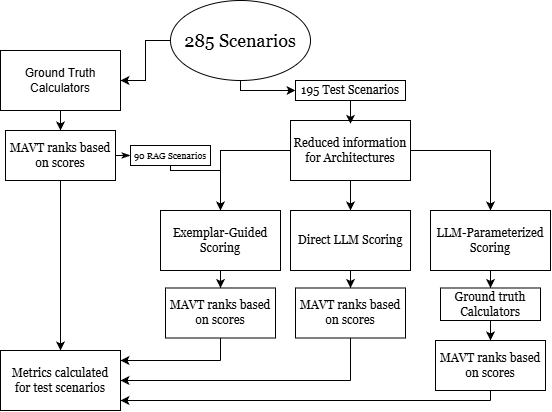
\includegraphics[width=0.5\textwidth]{FULLFlowMCDA.png}
  \caption{Decision-support workflow: scenario input $\rightarrow$ architecture-specific scoring or extraction $\rightarrow$ MAVT aggregation $\rightarrow$ ranked output.}
\label{fig:full-flow-mcda}
\end{figure}
Figure~\ref{fig:full-flow-mcda} shows the full decision-support workflow common to all three architectures. The three architectures differ only in how the scoring step is performed.
\FloatBarrier

Failed outputs are marked with a reserved sentinel value and excluded from metrics (Section~\ref{sec:eval-metrics}); imputed metrics under an alternative failure-handling rule appear in Appendix~\ref{app:imputed}.

Results are reported as five-run means $\pm$ standard deviations. Each architecture--model combination is run independently five times at temperature 0.3. Metrics (Kendall's $\tau$, MAE, RMSE, Top-1 accuracy) are computed independently for each run, then averaged across the five runs. This per-run-then-average protocol measures the expected performance of a single deployment; the per-run standard deviation quantifies run-to-run stability. Appendix~\ref{app:method-c} reports mean-aggregate consensus results.

Table~\ref{tab:parameter_comparison} details the parameters given to architectures vs.\ calculators, shown for HVAC as the illustrative case.
\begin{table}[H]
\begin{threeparttable}
\centering
\footnotesize
\renewcommand{\arraystretch}{0.88}
\caption{Scenario parameters available to LLM architectures vs.\ ground-truth calculators (HVAC).}
\label{tab:parameter_comparison}
\centering
\begin{tabular}{@{} l c c @{}}
\toprule
\textbf{Parameter} & \textbf{LLMs} & \textbf{Calc.} \\
\midrule
Location            & \checkmark & ---        \\
Outdoor Temp        & \checkmark & \checkmark \\
Home Size (sq ft)   & \checkmark & \checkmark \\
Insulation Tier$^{a}$   & \checkmark & ---        \\
R-Value             & ---        & \checkmark \\
Household Size      & \checkmark & \checkmark \\
Housing Type        & \checkmark & \checkmark \\
House Age$^{b}$     & \checkmark & \checkmark \\
Utility Budget      & \checkmark & \checkmark \\
SEER Rating         & ---        & \checkmark \\
Occupancy Context$^{c}$   & \checkmark & \checkmark \\
Indoor Temp (alt.)  & ---        & \checkmark \\
\bottomrule
\end{tabular}
\begin{tablenotes}
\footnotesize
\item[a] Tier labels (Poor/Medium/Good) map to R-value ranges; see \S\ref{sec:gt-calculators}.
\item[b] LLMs receive a building-age range label (e.g., ``20+ Years''); the calculator uses exact HVAC age.
\item[c] Question context provides occupancy information.
\end{tablenotes}
\end{threeparttable}
\end{table}

\FloatBarrier

Appliance and Shower parameters follow the same visible/hidden split (full tables in Appendix~\ref{app:parameter_comparison_full}). The parameters given to the LLM architectures are chosen as they are parameters readily observable by a household occupant \cite{doehesscore2021}.



Each insulation tier spans a range of R-values drawn from standard U.S.\ residential wall assemblies \cite{cec_ja43_2013,energystar_insulation2023}: Poor scenarios use R-8 to R-12 (minimal 2$\times$4 cavity fill, below current code), Medium scenarios use R-13 to R-18 (standard 2$\times$4 batt through 2$\times$6 mixed), and Good scenarios use R-19 to R-24 (2$\times$6 framing and above). The tier boundaries are chosen so that adjacent tiers differ by 15--20\% in wall R-value, matching the minimum difference a homeowner could detect by inspecting cavity depth. SEER ratings in the test corpus span 8--22, covering pre-1992 units (SEER~8--10), standard-efficiency replacements (SEER~13--14), and high-efficiency models (SEER~16--22), consistent with the ENERGY STAR Most Efficient threshold \cite{energystar_ac2023}.

Appliance age bands (1--3, 4--6, 7--9, 10--12, 13--17, 18--22 years) map to measured kWh/cycle ranges drawn from the ENERGY STAR certified-products database, so that a ``7--9 year'' dishwasher maps to the same energy draw whether the true age is 7 or 9. Housing type (apartment, condo, townhouse, rowhouse, twin, single-family) determines the envelope multiplier in the HVAC load equation and the noise propagation factor in the appliance comfort model; these mappings are detailed in Section~\ref{sec:gt-calculators}.

For the Flow Rate parameter, the scenario's numeric GPM is bucketed into three qualitative labels: \texttt{low\_flow} ($\le$2.0\,GPM, including EPA WaterSense certified 1.5\,GPM showerheads \cite{epawatersense}), \texttt{standard} (2.5--3.0\,GPM, at or near the Energy Policy Act of 1992 federal maximum of 2.5\,GPM \cite{epawatersense}), and \texttt{high\_flow} ($>$3.0\,GPM). The label is shown to the LLM; the calculator always receives the exact numeric GPM from the scenario.

The $\mathcal{A}_{\text{H}}$ architecture instead extrapolates these parameters from context before invoking the calculator (Section~\ref{sec:architectures}). The benchmark therefore measures whether $\mathcal{A}_{\text{H}}$ can bridge the gap between a fully specified reference calculator and the incomplete information a household could realistically provide.

\subsection{MAVT Framework \& Weighting Design}
\label{sec:mavt-design}
The Multi-Attribute Value Theorem (MAVT) allows alternatives to be compared on different criteria based on the range of values that occurs for each criterion \cite{keeneyraiffa1976,dyer1979}.

The weights USED are held constant across all decision types, all architectures, and the ground-truth calculator. We did this so that any difference in score is because of the inputs and value function, not because of difference in the way each criterion is perceived for the three decision types. Normally, MAVT additive form (Eq.~\ref{eq:mavt_sum}) requires preferential independence among criteria \cite{dyer1979,keeneyraiffa1976}. This means that criteria should be independent, meaning that the value (good or bad) of one criterion should have no effect on the value of another criterion.

\begin{equation}
\label{eq:mavt_sum}
s_j = \sum_{i=1}^{4} w_i \cdot v_i(x_{ij})
\end{equation}

In the case of our criteria, the energy cost and the environmental impact criterion are not completely independent, as they both stem from the kWh usage of an activity; The Spearman's rho between energy cost and environmental impact is 0.92. However, this is a feature of the dataset and of household emissions, and it is actually possible for the two criteria to diverge. Since environmental impact comes from actual CO\textsubscript{2}, which varies based on the type of power plant generating the power, grid mix composition, renewable penetration, and regional interconnection flows \cite{pjm2022emissions}, and energy cost comes from the time of day, gas peakers, demand charges, transmission congestion pricing, and utility revenue requirements \cite{peco2021}. While Pennsylvania does not usually have such divergence, there are other areas that do. CAISO (California ISO), for example, exhibits this divergence daily: during midday solar oversupply, wholesale prices routinely turn negative, yet marginal emissions remain low because solar is on the margin; by contrast, during the evening ramp, natural-gas peakers set the marginal price and marginal emissions simultaneously, creating periods where low-cost and high-emission conditions cannot co-occur \cite{caiso2025duck,ascend2025}.

In our study, we chose the following weights: Environmental Impact (35\%), Energy Cost (30\%), Comfort (20\%), and Practicality (15\%), as summarized in Table~\ref{tab:item3}.

\begin{table}[htbp]
\begin{threeparttable}
\small
\centering
\renewcommand{\arraystretch}{1.15}
\begin{tabular}{lllll}
\toprule
Criterion & Weight (\%) & Value Function & $\alpha$ & Direction \\
\midrule
Environmental Impact & 35 & Linear (Eq.~\ref{eq:linear_vf}) & \textemdash & Lower raw = better \\
Energy Cost & 30 & Linear (Eq.~\ref{eq:linear_vf}) & \textemdash & Lower raw = better \\
Comfort & 20 & Logarithmic (Eq.~\ref{eq:log_vf}) & 1.5 & Higher raw = better \\
Practicality & 15 & Logarithmic (Eq.~\ref{eq:log_vf}) & 1.2 & Higher raw = better \\
\bottomrule
\end{tabular}
\renewcommand{\arraystretch}{1.0}
\caption{MAVT criterion specification. Weights sum to 100\% and are held constant across all architectures and the ground truth calculator.}
\label{tab:item3}
\end{threeparttable}
\end{table}

The Environmental Impact weight of 0.35 reflects two considerations. Residential emissions account for a sizable share of national CO\textsubscript{2} emissions \cite{dietz2009}, so a household decision-support tool that does not give priority to environmental impact fails in its objective. The Value--belief--norm theory, which says that environmental orientation is the most consistent normative driver across pro-environmental household behaviours, also applies heavily due to the nature of the people using the tool. \cite{stern1999,steg2005}. Finally, entropy-based normalization of the scenario distributions assigns higher information weight to the environmental criterion, independently supporting an above-average allocation \cite{roszkowska2026} (see ~\ref{app:weights} for the full computation).

 Weighting Energy Cost at 0.30 keeps it slightly below environmental impact while keeping its role as the criterion households actually act on; for the average person, cost is the strongest predictor of consumer adoption. In fact, cost savings as shown on energy labels for consumer products were even more effective than actual energy cost and carbon emissions \cite{newell2014}. For HVAC decisions, thermostat setpoints determine electricity draw at the billing rate, and households respond by reducing the difference from outside temperature whenever they can \cite{managementscience_pricing2023}. For appliance decisions, energy cost depends on the time-of-use rate at which the appliance runs; a dishwasher shifted from peak to off-peak can cut its per-cycle cost by 30--50\%, making cost the criterion most responsive to scheduling changes. For shower decisions, water heating accounts for a significant share of residential energy costs and the per-shower increment is rarely visible to users, amplifying the underestimation bias found by Attari et al. and making cost-feedback interventions similarly effective.  \cite{reu2016,harrispoll2024}.

Comfort is weighted at 0.20. Thermal comfort is the second driver of HVAC behavior \cite{aqilah2022,karjalainen2007}. The set points used for HVAC comfort were based mainly off of ASHRAE 55 \cite{ashrae55,dedear2002}. For appliance decisions, comfort is primarily a function of run-time delay: demand-response research finds that household willingness to accept a shift decays sharply beyond two to four hours, with dishwashers tolerated longest and dryers shortest \cite{paetz2012,waseem2020}, and the penalty scales further with household size as dishes and laundry accumulate faster. For shower decisions, comfort peaks around the REU2016 average of 7.8\,minutes \cite{reu2016,harrispoll2024} and depends additionally on temperature adequacy, with heater setpoints below CDC Legionella thresholds carrying a comfort penalty \cite{cdc2026}.

Practicality is weighted at 0.15. In our context, practicality means the likelihood that an activity will be continued long term. While this is partially linked to the other criterion, it also requires that the tool adds minimum friction relative to the existing routine. Otherwise, adoption of the tool drops \cite{ariely2001,leclerc1995,gardner2020,mergelsberg2020}. The lower weight (relative to comfort) is due to the fact that most of the decisions recommended by the tool are not likely to be repeated long-term or followed exactly. Additionally, practicality is a constraint on what is reasonable rather than a true user preference. Where comfort captures what a household would prefer given no constraints, practicality captures what is feasible and sustainable to adopt. A 15-minute shower may score near-optimally on comfort, but if four occupants share a 40-gallon tank, available hot water runs out before the third person showers---making that alternative infeasible regardless of comfort preference.

By requiring a score or parameter estimate for each of the four criteria, the structured framework prevents the LLM from arbitrarily selecting an alternative based on a single dominant attribute, a known failure mode of unaided LLM judgment \cite{wang2024fairescalers}.

\begin{equation}
\label{eq:linear_vf}
v_i(x) = \frac{x - x_{\min}}{x_{\max} - x_{\min}}
\end{equation}

The environmental and energy cost functions use the linear value function (Eq.~\ref{eq:linear_vf}) because equal absolute changes in these quantities represent equal improvements: a 1\,lb\,CO\textsubscript{2} reduction is equally valuable regardless of the baseline, and a \$0.10 saving carries the same decision weight at any cost level relative to the household's budget range \cite{dyer1979,keeneyraiffa1976}. Framing environmental impact in absolute physical units (lbs\,CO\textsubscript{2}) makes a linear preference the conservative modeling choice that treats identical emission reductions as equally desirable \cite{keeneyraiffa1976}.

\begin{equation}
\label{eq:log_vf}
v_i(x) = \frac{\ln\!\left(1 + \alpha \cdot \frac{x - x_{\min}}{x_{\max} - x_{\min}}\right)}{\ln(1 + \alpha)}
\end{equation}

The comfort and practicality criteria use the logarithmic value function (Eq.~\ref{eq:log_vf}) because both exhibit diminishing marginal returns: initial improvements from an uncomfortable or impractical baseline yield disproportionately large perceived gains, while incremental improvements near the optimum matter progressively less. For comfort, moving from a temperature far outside the ASHRAE~55 band toward the neutral setpoint produces large subjective gains, but further refinement within an already acceptable range has little additional effect \cite{ashrae55,dedear2002}. For practicality, adopting a behavior that fits within budget and routine constraints is a large step; further reducing friction beyond an already feasible option adds minimal value \cite{ariely2001,leclerc1995}. The shape parameter $\alpha = 1.5$ for comfort and $\alpha = 1.2$ for practicality were calibrated so that moderate gains (e.g., moving from the 25th to the 50th percentile of the criterion range) receive meaningful credit without over-rewarding marginal further improvements, while keeping the function close enough to linear that the difference in weights---rather than curvature---remains the dominant driver of the final MAVT score.

\subsection{Reference Ranges}

The reference ranges in Table~\ref{table:reference_ranges} are computed as the 5th--95th percentiles of the ground-truth quantity distributions over the scenario corpus (cost and emissions for HVAC and Appliance; cost and water volume for Shower), rather than extreme theoretical limits, so that normalization preserves meaningful spread across typical residential alternatives. However, since these values were used based on actual setpoints from Pennsylvania, they do reflect real world usage. Using dataset percentiles rather than the full theoretical physics envelope is a deliberate modeling choice \cite{roszkowska2026} at the cost of truncating scores for extreme outlier scenarios. The endpoints below are the percentile values to two decimals.

\begin{table}[H]
\begin{threeparttable}
\centering
\small
\caption{Reference ranges (5th--95th percentiles). Shower Environmental Impact is reported in gallons of water; HVAC and Appliance in lbs CO\textsubscript{2}.}
\label{table:reference_ranges}
\begin{tabular}{@{}lccc@{}}
\toprule
\textbf{Criterion} & \textbf{HVAC} & \textbf{Appliance} & \textbf{Shower} \\
\midrule
Energy Cost (\$) & 0.38--3.29 & 0.025--0.71 & 0.14--1.14 \\
Environmental Impact & 1.96--18.04 & 0.288--3.643 & 6.0--45.0 \\
Comfort & 0.0--1.0 & 0.0--1.0 & 0.0--1.0 \\
Practicality & 0.05--1.0 & 0.05--1.0 & 0.05--1.0 \\
\bottomrule
\end{tabular}
\end{threeparttable}
\end{table}

For HVAC, cost percentiles reflect active-conditioning alternatives. A setpoint near outdoor temperature produces zero decision-period load and collapses to \$0, which makes the lower bound go to zero. The cost is estimated at \$0.19/kWh, which represents a bundled retail rate combining generation, transmission, distribution, monthly service fees, riders, and state taxes. Form EIA-861 reports a 2024 Pennsylvania statewide average price of 17.77\textcent/kWh based on total utility revenue divided by sales \cite{eia_epa_2024}. However, in urban and suburban Philadelphia, the Pennsylvania Public Utility Commission 2025 Rate Report lists an average monthly PECO residential bill of \$135.29 for 702\,kWh, establishing an effective bundled price of 19.27\textcent/kWh \cite{paupc2025}. Approved PUC rate settlements increase representative 700\,kWh PECO bills to \$149.43 in 2025 (21.3\textcent/kWh) and \$152.13 in 2026 (21.7\textcent/kWh) \cite{paupc2024dec}. The \$0.19/kWh baseline provides a conservative, empirical rate for Pennsylvania decision modeling. Excluding zero-load points, the realized 8-hour cost distribution at Pennsylvania's bundled residential rate (\$0.19/kWh) \cite{eia_epa_2024,paupc2025,paupc2024dec} spans \$0.38--\$3.29.  An Off option receives top cost score via decreasing-value normalization. These endpoints match residential HVAC efficiency benchmarks \cite{synapse2013,parker2018}. 

Using this kWh distribution with PJM marginal emissions factors (0.976 off-peak, 1.041 peak lbs CO\textsubscript{2}/kWh) yields HVAC environmental bounds of 1.96--18.04 lbs CO\textsubscript{2} \cite{pjm2022emissions}. 


For appliances, the realized per-cycle cost distribution (kWh/cycle multiplied by the resolved time-of-use rate across the six PA utilities) spans \$0.025--\$0.71, and the realized per-cycle emissions distribution (kWh/cycle through the PJM marginal factor at run time) spans 0.288--3.643 lbs CO\textsubscript{2}. The underlying per-cycle energy endpoints remain consistent with the ENERGY STAR certified-products distribution (efficient HE washers near 0.25\,kWh) and include the older non-certified electric resistance dryers \cite{energystar_products,chenyu2018,hustvedt2013,neep2015,porras2020}.

For showers, the realized per-shower cost distribution spans \$0.14--\$1.14. Shower energy follows the mixing-fraction physics targeting a fixed 105\,\textdegree{}F delivery temperature, so it depends only on the rise from the mains inlet (seasonal inlet temperatures from NREL hot-water modeling \cite{hendron2008}) to that target and is independent of heater setpoint; cost is this energy priced at the PA residential rate. 

Shower environmental impact is defined as water volume (gallons); the realized distribution of flow rate multiplied by duration spans 6.0--45.0 gallons at the 5th--95th percentile, with flow-rate and duration benchmarks from EPA WaterSense Appendix~B \cite{epawatersense}, REU2016 \cite{reu2016}, and The Harris Poll \cite{harrispoll2024}. This was done as opposed to using simple carbon dioxide because CO\textsubscript{2} estimates would reduce the level of seperation between the Environmental and Energy Cost criteria. 

\subsection{Ground Truth Calculators}
\label{sec:gt-calculators}
Each ground-truth calculator consumes a scenario with three alternatives and returns four scores per alternative---Energy Cost (\$), Environmental Impact, Comfort, and Practicality---plus the raw physical quantities for environmental impact and energy cost before value-function transformation. Energy cost is in dollars per 8-hour decision period (HVAC), per cycle (Appliance), or per shower (Shower); monthly estimates are computed only for the budget penalty; Environmental Impact is in lbs\,CO\textsubscript{2} for HVAC and Appliance decisions and in gallons of water for Shower decisions.

For HVAC and Appliance decisions, environmental impact uses PJM marginal emissions factors:
\begin{equation}
  \mathrm{CO_2} = E_{\mathrm{kWh}} \cdot \varepsilon(t), \qquad
  \varepsilon(t) = \begin{cases}
    1.041 \text{ lbs/kWh} & \text{peak (7am--11pm)} \\
    0.976 \text{ lbs/kWh} & \text{off-peak}
  \end{cases}
  \label{eq:emissions}
\end{equation}
\noindent where $E_{\mathrm{kWh}}$ is the decision-period energy use and $\varepsilon(t)$ is the PJM marginal emissions factor at run time $t$ \cite{pjm2022emissions}. Marginal rather than average factors are used because shifting a residential load displaces or adds the generator at the margin.
All three calculators apply an identical four-tier budget penalty $P(u)$ multiplicatively to the energy-cost value-function output, where $u = C_{\mathrm{monthly}} / B$ is monthly cost utilization relative to the household's stated budget $B$:
\begin{equation}
  P(u) = \begin{cases}
    1.0                          & u < 0.80                   \\[4pt]
    1 - 2.5\,(u - 0.80)         & 0.80 \le u < 1.0           \\[4pt]
    0.5\,e^{-3(u - 1.0)}        & 1.0 \phantom{0}\le u < 1.5 \\[4pt]
    0                            & u \ge 1.5
  \end{cases}
  \label{eq:budget_penalty}
\end{equation}
\noindent where $P(u)$ is a unitless multiplicative penalty on the (post value-function) energy-cost score, $u$ is monthly budget utilization, $C_{\mathrm{monthly}}$ is estimated monthly energy/water-related cost for the decision type, $B$ is the household-stated monthly budget for utilities, and $e$ is Euler's number.
\noindent The no-penalty zone ($u < 0.80$) reflects mental budget safety margins \cite{thaler1999}; the linear decline approaching the limit follows Heath \& Soll's budget self-control model \cite{heath1996}; exponential loss aversion for overruns follows Prelec \& Loewenstein \cite{prelec1998} and Heutel \cite{heutel2017}; and elimination beyond 150\% reflects financial infeasibility \cite{gathergood2012}. Applying the penalty multiplicatively ensures extremely cheap or expensive alternatives cannot completely sway ranking on energy cost alone.

\noindent For HVAC decisions, $C_{\mathrm{monthly}} = 90\,C_{\mathrm{8h}}$, where $C_{\mathrm{8h}}$ is the energy cost for one 8-hour conditioning period and 90 is three such periods per day across 30 days. The Appliance and Shower monthly-cost conversions are given in Eq.~\ref{eq:appliance_monthly_cost} and Eq.~\ref{eq:shower_monthly_cost}.

\subsubsection{HVAC Calculator}
Thermal load decomposes into four ASHRAE-style components. For cooling:
\begin{equation}
  Q_{\mathrm{cool}} =
    \underbrace{\frac{m \cdot A}{R}\,\Delta T}_{\text{conductive}}
    +\underbrace{400n + A + 800}_{\text{internal}}
    +\underbrace{0.15\,A \times 20}_{\text{solar}}
    +\underbrace{1.08\,\frac{A\, h_c\, \alpha}{60}\,\Delta T}_{\text{infiltration}}
  \label{eq:hvac_cooling_load}
\end{equation}
\noindent where $A$ is floor area (sq\,ft); $m$ is a housing-type envelope multiplier (1.7 single-family, 1.6 twin/semi-detached, 1.5 townhouse/rowhouse, 1.2 apartment/condo) \cite{accamanualj}; $R$ is the wall insulation R-value; $\Delta T = T_{\mathrm{out}} - T_{\mathrm{in}}$; $n$ is household size; $h_c = 8$\,ft and $\alpha = 0.35$\,ACH for ceiling height and infiltration rate \cite{polly2011}. The 800\,BTU/hr baseline captures always-on standby loads per ACCA Manual~J \cite{accamanualj}. The heating load uses the same expression with $\Delta T = T_{\mathrm{in}} - T_{\mathrm{out}}$, no solar term, and internal gains subtracted rather than added.

Effective EER is estimated from the unit's rated SEER via the AHRI\,210/240 quadratic \cite{ahri2008}:
\begin{equation}
  \mathrm{EER} = -0.02\,\mathrm{SEER}^{2} + 1.12\,\mathrm{SEER}
  \label{eq:eer_quadratic}
\end{equation}
\noindent where $\mathrm{SEER}$ is the unit's rated seasonal energy efficiency ratio and $\mathrm{EER}$ is the resulting effective energy efficiency ratio used for the decision period. Age- and maintenance-driven efficiency degradation is deliberately \emph{not} applied to the energy path; it is instead modeled as a reliability factor in the practicality score (Eq.~\ref{eq:hvac_degradation}), so the energy score reflects the setpoint choice rather than the system's condition. Energy consumption over the 8-hour decision window is then:
\begin{equation}
  E_{\mathrm{kWh}} =
    \frac{Q_{\mathrm{load}}}{\mathrm{EER} \times 1000}
    \cdot 8 \cdot m_{\mathrm{occ}}
  \label{eq:hvac_energy}
\end{equation}
\noindent where $Q_{\mathrm{load}}$ is the thermal load (BTU/hr) for the decision context and $m_{\mathrm{occ}}$ scales for occupancy context: 1.0 for fully occupied, 0.75 for overnight, and $1 - 0.5(h_{\mathrm{away}}/24)$ for daytime unoccupied periods \cite{houde2021}, where $h_{\mathrm{away}}$ is hours-away per 24-hour day.

Because HVAC alternatives carry no explicit run-time, the marginal emissions factor in Eq.~\ref{eq:emissions} is resolved from the occupancy context by applying each pattern onto the PJM peak (7am--11pm, 16\,h) and off-peak (8\,h) windows, with away-hours assumed to fill the daytime peak window first:
\begin{equation}
  \varepsilon_{\mathrm{occ}} =
  \begin{cases}
    \varepsilon_{\mathrm{off}} & \text{occupied-sleep (night-only runtime)} \\[4pt]
    \dfrac{16\,\varepsilon_{\mathrm{pk}} + 8\,\varepsilon_{\mathrm{off}}}{24}
      & \text{occupied all day} \\[8pt]
    \varepsilon_{\mathrm{pk}} & \text{unoccupied } H\text{\,hr},\; H \le 16 \\[4pt]
    \dfrac{16\,\varepsilon_{\mathrm{pk}} + (H-16)\,\varepsilon_{\mathrm{off}}}{H}
      & \text{unoccupied } H\text{\,hr},\; H > 16
  \end{cases}
  \label{eq:hvac_occ_emissions}
\end{equation}
\noindent where $\varepsilon_{\mathrm{pk}} = 1.041$ and $\varepsilon_{\mathrm{off}} = 0.976$\ (in terms of lbs/kWh) are the PJM peak and off-peak marginal factors and $H$ is hours-away per day \cite{pjm2022emissions}. Occupied-sleep returns the off-peak factor because the home's conditioning runtime falls entirely in the overnight off-peak window.

Comfort uses a tent function anchored to ASHRAE\,55 PMV-optimal setpoints \cite{ashrae55_2020,vanhoof2008,fanger1970}:
\begin{equation}
  C_{\mathrm{comfort}} = \tfrac{1}{10}\max\!\Bigl(0,\; 10 - \lvert T_{\mathrm{in}} - T^{*}\rvert - \tfrac{(n-3)\,0.3\,\lvert T_{\mathrm{in}} - T^{*}\rvert}{3}\Bigr)
  \label{eq:hvac_comfort}
\end{equation}
\noindent where $C_{\mathrm{comfort}}$ is a 0--1 comfort score, $T_{\mathrm{in}}$ is the indoor setpoint, $T^{*}$ is the context-dependent optimal setpoint used as the peak of the tent function ($76$\,\textdegree{}F in cooling mode, $70$\,\textdegree{}F in heating mode, consistent with ASHRAE\,55-2020 sedentary PMV bands \cite{ashrae55_2020}). The penalty term applies only for household sizes $n > 3$, and $n$ is household size.
Practicality utility follows a piecewise value function of setpoint extremity, indoor--outdoor $\Delta T$, and equipment age. This is the first of five comfort and practicality utilities defined this way across the three calculators; full derivations for all of them are in Appendix~\ref{app:utility_derivations}.

An ``Off'' alternative (no active conditioning) is scored with zero decision-period energy, cost, and emissions; its comfort and practicality are instead evaluated against the free-float indoor temperature the building drifts to with the system off --- outdoor $+5$\,\textdegree{}F in cooling season and $+10$\,\textdegree{}F in heating season, reflecting solar and internal gains that hold a closed, occupied house above outdoor air temperature \cite{dedear2002,ashrae55_2020,accamanualj,ashrae_hof2017}.

\subsubsection{Appliance Calculator}
Energy cost per cycle is

\begin{equation}
    C = E_{\mathrm{cyc}} \cdot r(t,\ell)
\end{equation}

where $E_{\mathrm{cyc}}$ is kWh/cycle and $r(t,\ell)$ is the location- and time-specific TOU rate resolved to one of six Pennsylvania utilities (PECO, PPL, West Penn, Penelec, MetEd, Duquesne) \cite{peco2021} (see \ref{app:tou_rates} for the full rate structure).
\noindent. $C$ is per-cycle energy cost (dollars/cycle), $E_{\mathrm{cyc}}$ is per-cycle energy use (kWh/cycle), $t$ is the appliance run time (time-of-day), and $\ell$ is the household location used to resolve the serving utility.

The PJM emissions window (7am--11pm) applies to environmental impact regardless of the utility's billing window, because emissions follow the regional grid.
The run-time rate period is selected by mapping location $\ell$ to a utility $U(\ell)$ and then applying that utility's TOU peak window otherwise.
\begin{equation}
(h^{U}_{\mathrm{pk,s}}, h^{U}_{\mathrm{pk,e}}):
\quad
r(t,\ell)=r^{U}_{\mathrm{pk}}
\text{ if }
h(t)\in[h^{U}_{\mathrm{pk,s}}, h^{U}_{\mathrm{pk,e}})
\text{ and }
r(t,\ell)=r^{U}_{\mathrm{off}}
\end{equation}
\noindent where $U(\ell)$ maps location $\ell$ to a serving utility, $h^{U}_{\mathrm{pk,s}}$ and $h^{U}_{\mathrm{pk,e}}$ are that utility's TOU peak-window start and end hours, $r^{U}_{\mathrm{pk}}$ and $r^{U}_{\mathrm{off}}$ are the utility's peak and off-peak energy prices (\$/kWh), and $h(t)$ maps time $t$ to an hour-of-day on a 24-hour clock.
\noindent In the implementation, the six utilities use distinct peak windows (e.g., 2--6pm for PECO and PPL, 2--9pm for most FirstEnergy utilities). The appliance calculator does not model weekend or holiday peak-hour pricing; all days use weekday TOU rates. Seasonal peak-window shifts are also unmodeled: PPL's winter (Dec--May) peak window is 4--8pm versus the 2--6pm summer window applied here; the summer window is used year-round because scenarios carry no season or date field. This simplification shifts the optimal scheduling window by 1--2 hours for some utilities in winter months.

Comfort utility is parameterized by delay, appliance type, housing type, and household size; practicality utility by delay, run-time hour, and household coordination difficulty (Appendix~\ref{app:utility_derivations}).
For budget utilization in \eqref{eq:budget_penalty}, the appliance calculator converts per-cycle cost to a monthly estimate as:
\begin{equation}
  C_{\mathrm{monthly}} = c(\mathrm{type})\,C_{\mathrm{cycle}}, \qquad
  c(\mathrm{type})=
  \begin{cases}
    18 & \text{dishwasher} \\[2pt]
    25 & \text{washer} \\[2pt]
    24 & \text{dryer}
  \end{cases}
  \label{eq:appliance_monthly_cost}
\end{equation}
\noindent where $C_{\mathrm{cycle}}$ is per-cycle energy cost and $c(\mathrm{type})$ is the appliance-specific cycles-per-month estimate, from 215, 300, and 283 cycles/year for dishwashers, washers, and dryers respectively \cite{energystar_dishwasher_criteria2023,energystar_clotheswasher,doe_dryer_tp_2011}.

\subsubsection{Shower Calculator.}
Mains inlet temperature is interpolated from outdoor temperature between 45\,\textdegree{}F (winter, $T_{\mathrm{out}} \le 32$\,\textdegree{}F) and 65\,\textdegree{}F (summer, $T_{\mathrm{out}} \ge 75$\,\textdegree{}F) \cite{hendron2008,backman2013}. Only the fraction of flow requiring heating reaches the heater; that mixing fraction is:
\begin{equation}
  f_{\mathrm{hot}} = \frac{T_{\mathrm{target}} - T_{\mathrm{inlet}}}
                          {T_{\mathrm{heater}} - T_{\mathrm{inlet}}}
  \label{eq:shower_fraction}
\end{equation}
\noindent where $f_{\mathrm{hot}}$ is the fraction of total flow drawn as hot water, $T_{\mathrm{target}} = 105$\,\textdegree{}F is the standard comfortable delivery temperature \cite{zhang2023}, $T_{\mathrm{inlet}}$ is mains inlet temperature, and $T_{\mathrm{heater}}$ is the water-heater setpoint temperature. Shower energy is then:
\begin{equation}
  E_{\mathrm{kWh}} = \frac{\dot{V} \cdot f_{\mathrm{hot}} \cdot 8.33 \cdot
                            (T_{\mathrm{heater}} - T_{\mathrm{inlet}}) \cdot \tau}
                          {3412 \cdot \eta}
  \label{eq:shower_energy}
\end{equation}
\noindent where $E_{\mathrm{kWh}}$ is shower energy use (kWh), $\dot{V}$ is total flow rate (GPM), $\tau$ is shower duration (min), $\eta = 0.92$ is the unified energy factor for a 40--55\,gal electric tank \cite{rheem2025}, and $3412$\,BTU/kWh is the standard conversion; the constant $8.33$\,lb/gal converts gallons to pounds of water.

Environmental impact is water volume:
\begin{equation}
    V = \dot{V} \cdot \tau
    \label{eq:shower_volume}
\end{equation}
\noindent measured in gallons, where $\dot{V}$ is total flow rate (GPM) and $\tau$ is shower duration (min).

Energy cost uses a flat electricity rate $p_e$:
\begin{equation}
  C_{\$}=p_e\,E_{\mathrm{kWh}}.
  \label{eq:shower_cost}
\end{equation}
\noindent where $C_{\$}$ is shower energy cost (dollars) and $p_e$ is the electricity price (\$/kWh).
Comfort utility is parameterized by duration, heater setpoint, and household contention; practicality utility by duration and tank-capacity feasibility (Appendix~\ref{app:utility_derivations}).
For budget utilization in the budget penalty equation, shower monthly cost is estimated from per-shower cost using an average showers-per-person-per-day rate:
\begin{equation}
  C_{\mathrm{monthly}} = C_{\mathrm{shower}} \cdot \bigl(n \cdot 0.9 \cdot 30\bigr).
  \label{eq:shower_monthly_cost}
\end{equation}
\noindent where $C_{\mathrm{shower}}$ is per-shower energy cost, $n$ is occupants, $0.9$ is showers/person/day, and $30$ is days/month.

\subsection{Architecture Implementations}
\label{sec:architectures}
All three architectures call the same model per test via OpenRouter at temperature 0.3, a moderate value that balances instruction-following fidelity against output diversity, with model held constant within each run.
Temperature 0.0 amplifies any single-run extraction error into the final ranking, whereas 0.3 introduces controlled diversity that lets cross-run recovery filter out transient failures. The study evaluates four models spanning a range of capability, reasoning support, and cost: GPT-OSS-20B (\texttt{openai/gpt-oss-20b}, reasoning, low effort), Qwen 3.5 9B (\texttt{qwen/qwen3.5-9b}, non-reasoning), DeepSeek V4 Flash (\texttt{deepseek/deepseek-v4-flash}, hybrid reasoning), and Gemini 3.5 Flash (\texttt{google/gemini-3.5-flash}, reasoning, minimal effort). Each was set to its lowest possible reasoning tier. Alternative order in the prompt was fixed (alt-1, alt-2, alt-3 in scenario-sheet order) across all runs and was not randomized. Ties in the MAVT aggregate were broken deterministically by the priority order environmental, energy cost, comfort, practicality.

\begin{figure}[H]
	\centering
	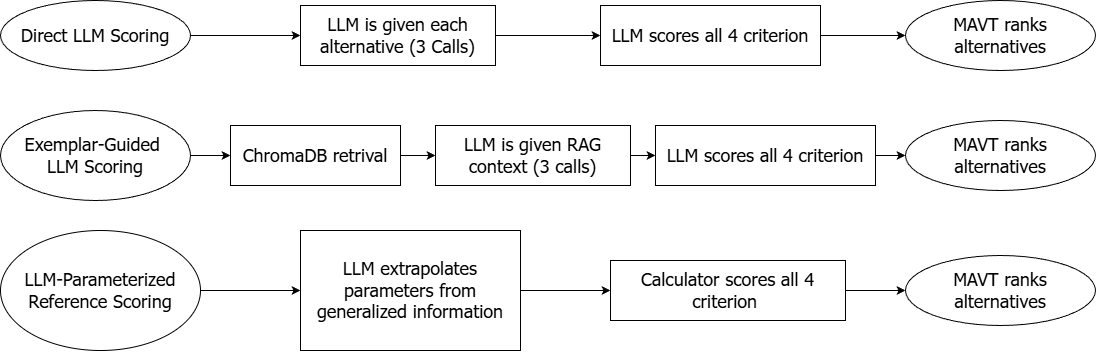
\includegraphics[width=1\textwidth]{ArchitectureFlowcharts.png}
  \caption{Processing pipeline for each architecture.}
\label{fig:pipeline}
\end{figure}

Figure~\ref{fig:pipeline} shows the processing pipeline for each architecture; the three architecture implementations are described below.



\subsubsection{\texorpdfstring{$\mathcal{A}_{\text{D}}$}{A_D} (Direct Prompting)}
The $\mathcal{A}_{\text{D}}$ architecture issues one API call per alternative (three calls per scenario) using a calibrated system prompt that combines role-prompting \cite{shanahan2023}, structured-output constraints \cite{wei2022cot}, and explicit bias-mitigation language drawn from the NIST framework for identifying and managing AI bias \cite{nistsp1270}. No external context is supplied beyond the scenario description. The system prompt establishes the analyst role and, for each of the three decision types, gives each of the four criteria a short anchor phrase describing what a good and a poor score look like on that criterion. It closes with a strict JSON-only output instruction and a reminder to distinguish between criteria, consistent with the bias-mitigation language cited above (full prompt text in Appendix~\ref{app:prompts}).

\noindent The user prompt provides the scenario context and asks the model to score one alternative at a time, including the other alternatives as reference so that it doesn't assign the same scores to all alternatives. 

%TODO: add a short in-text scoring example for one alternative, and explain the qualitative anchor design with citations to the sources noted beside each prompt in the repo.

\subsubsection{\texorpdfstring{$\mathcal{A}_{\text{E}}$}{A_E} (Example-Guided LLM Scoring)}
The $\mathcal{A}_{\text{E}}$ architecture retrieves the single most similar scenario ($k=1$) from a ChromaDB vector store before scoring, using the sentence-transformers/all-MiniLM-L6-v2 embedding model. The retrieval count $k=1$ was selected based on a development-set ablation (Section~\ref{sec:rag-ablation-methods}): all retrieval counts ($k=1,3,5$) produced statistically indistinguishable ranking accuracy, so $k=1$ was chosen as the production setting to minimize token and API cost within that equivalence cluster (full ablation results in Section~\ref{sec:rag-ablation}).

The ablation sample was stratified to cover the full parameter space, and the single closest exemplar showed a mean cosine distance of 0.05 across all scenarios, confirming that every scenario in a representative draw has a closely matching corpus entry. Because the RAG corpus was designed for complete parameter-space coverage (Section~2.1), this holds for the full test set: no scenario lacks a sufficiently similar exemplar, and additional retrieved examples provide no measurable benefit.

The retrieved exemplar is rendered as a full worked example: its household-reported parameters, its engineering parameters (R-value, SEER, GPM, kWh/cycle, tank size, heater setpoint, etc.), and each of its alternatives with the four ground-truth criterion scores plus the MAVT aggregate and rank. The exemplar's engineering values are shown so the model can see how those values map to scores. The model is instructed to use the exemplar as reference but to score the target scenario independently. Like $\mathcal{A}_{\text{D}}$, $\mathcal{A}_{\text{E}}$ uses three API calls per scenario (one per alternative). The retrieval index is built once from the 90 RAG-only scenarios described in Section~2.1; test scenarios are used only as query vectors and the index stores only RAG scenarios \cite{lewis2020}.

The system prompt is identical to $\mathcal{A}_{\text{D}}$ but omits the per-criterion anchor descriptions, since the RAG exemplars supply implicit scoring guidance in their place; it keeps the same JSON-only output format and criteria-distinction instruction (full prompt text in Appendix~\ref{app:prompts}).

\noindent A retrieved HVAC exemplar (engineering parameters and ground-truth scores included) is rendered as:

\begin{alltt}
\small
RELEVANT SIMILAR SCENARIOS WITH EXPERT SCORES:

Example 1:
  Question: What temperature should I set my thermostat to?
  - Location: Chicago
  - Outdoor Temp: 95 deg F
  - Square Footage: 2000 sqft
  - Insulation: Medium
  - Household Size: 3 occupants
  - Housing Type: Single-Family
  - House Age: 6-10 years
  - R-Value: 13
  - SEER: 14
  - HVAC Age: 8 years
  - Utility Budget: \$200/month
  Expert scores:
  * 76 F: Energy Cost: 0.4/1, Environmental: 0.3/1,
    Comfort: 0.9/1, Practicality: 0.8/1
    | MAVT: 0.58, Rank: 2
  * 78 F: Energy Cost: 0.6/1, ...
Use these examples as reference, but score based on
the specific scenario above.
\end{alltt}

\vspace{0.3em}

\noindent The user prompt presents the target scenario, the alternative to score, and the retrieved exemplar---with household-reported parameters, engineering values, and the four ground-truth scores plus MAVT aggregate and rank---instructing the model to ``consider how this specific alternative performs given the scenario context.'' 

\subsubsection{\texorpdfstring{$\mathcal{A}_{\text{H}}$}{A_H} (LLM-Parameterized Reference Scoring)}
The $\mathcal{A}_{\text{H}}$ architecture issues a single API call per scenario for structured parameter extraction. Known household-reported scenario fields (outdoor temperature, square footage, insulation tier, household size, housing type, utility budget, and location) are passed directly to the calculator without LLM involvement, and the three alternatives are taken verbatim from the scenario sheet---the deterministic calculator, not the LLM, parses the numeric content of each alternative string (setpoint temperature, run time, or shower duration). The LLM is asked only to estimate the genuinely withheld engineering parameters that are absent from the household-reported description: for HVAC, the wall R-value, SEER rating, HVAC age, and occupancy context; for Appliance, the appliance type, kWh/cycle, and current baseline time; for Shower, the numeric GPM (estimated from the household-reported flow-rate label), tank size, and water-heater setpoint.

The extracted JSON is validated before execution. A validation script checks extracted parameters against physical limits: HVAC wall R-value (1.0--60.0), SEER (6.0--30.0), equipment age (0.0--60.0 years); appliance energy (0.05--10.0 kWh/cycle); and shower flow rate (0.5--8.0 GPM), tank capacity (10.0--120.0 gallons), and water heater setpoint (80.0--160.0\,$^\circ\text{F}$). If an LLM predicts an out-of-range value or returns non-numeric text, the script marks the extraction as a failure rather than passing bad inputs to the calculator. Validated parameters are merged with the known fields and passed to the corresponding ground-truth calculator.

The extraction prompt uses decomposed prompting \cite{khot2023} to separate natural-language understanding from quantitative computation: unlike $\mathcal{A}_{\text{D}}$ and $\mathcal{A}_{\text{E}}$, it does not ask the LLM to score alternatives, only to extract the withheld engineering parameters into a fixed per-decision-type JSON schema, with an explicit instruction to estimate rather than omit any mandatory field (full prompt text in Appendix~\ref{app:prompts}).

Because the parameters the LLM estimates are scenario-level and identical across the three alternatives, most estimation errors occur in all three raw values together and largely cancel in ranking; ranking accuracy is therefore expected to be robust to weak extraction, whereas the score-level error (MAE/RMSE) and the per-alternative appliance baseline time are the measures that will actually reveal the quality of the extraction.

\subsection{RAG Ablation Design}
\label{sec:rag-ablation-methods}
Ablation experiments use the complete 90-scenario RAG corpus under a leave-one-out protocol: each scenario is used as the query with itself excluded from retrieval, since the corpus scenarios serve as both queries and retrieval index. Seven configurations modify one design variable at a time against a $k=3$ control: retrieval $k$ (1, 5), embedding model (paraphrase-MiniLM-L3-v2 replacing all-MiniLM-L6-v2), exemplar content (hidden engineering parameters included/excluded), score anchoring (scores and ranks present/absent), random exemplar selection (replacing similarity-ranked exemplars with random corpus draws), and a nearest-neighbor offline baseline that assigns retrieved scenario scores directly without LLM rescoring.

Each configuration is evaluated across three models. The $k=1$ variant tests whether a single high-similarity exemplar provides sufficient guidance; $k=5$ tests whether broader context improves or dilutes the signal. The embedding-swap tests a different matching architecture. The exemplar-content variants isolate whether the model benefits from seeing the engineering parameters (R-value, SEER, GPM, kWh/cycle) or only the household-reported labels. The score-anchoring variants test whether the model uses the ground-truth scores as calibration anchors or merely as noise. The random-exemplar variant controls for retrieval quality: if retrieval similarity matters, random exemplars should perform worse than similarity-ranked ones. The nearest-neighbor offline baseline tests whether unmodified exemplar copying provides ranking signal.

A Friedman test is run per metric (Kendall's $\tau$, Top-1 accuracy, MAE, RMSE) across all seven configurations pooled over models, giving a four-test family; Holm correction is applied across this family before any omnibus result is treated as significant, and post-hoc pairwise Wilcoxon signed-rank tests, themselves Holm-corrected within their own pairwise family, are computed only for the metrics whose corrected omnibus remains significant. (The prompt and hybrid ablations below use the same two-stage Friedman$\to$Holm$\to$Wilcoxon protocol, applied to their own strata.) Post-hoc pairwise comparisons confirm that all retrieval counts, the alternate embedding, and the exemplar-content variant form a statistically indistinguishable cluster on score MAE, while removing exemplar scores or using random retrieval significantly degrades performance. Based on this equivalence, $k=1$ was selected as the production retrieval count: it matches the ranking accuracy of $k=3$ and $k=5$ at the lowest token and API cost (full ablation results in Section~\ref{sec:rag-ablation}).

\subsection{Prompt Ablation Design}
\label{sec:prompt-ablation-methods}
A separate ablation tests whether the results depend on the specific prompts used to implement $\mathcal{A}_{\text{D}}$ and $\mathcal{A}_{\text{E}}$ rather than on the architectures themselves. Three perturbations modify one prompt property at a time against the shipped control: removing the numeric anchors that define the endpoints of the scoring scale (no\_anchors), inserting an explicit chain-of-thought scaffold that instructs the model to reason before emitting JSON (cot\_scaffold), and rescaling the response range from 0--1 to 0--10 with scores divided by ten before scoring (scale\_0\_10). Each variant runs on all 195 Test scenarios across three models with five runs per cell, holding criterion weights, temperature, and the scenario set fixed. $\mathcal{A}_{\text{E}}$ ships without numeric anchors in its prompt, so no\_anchors applies only to $\mathcal{A}_{\text{D}}$; the resulting matrix has 105 cells rather than 120. $\mathcal{A}_{\text{H}}$ is excluded because its LLM call extracts engineering parameters rather than emitting criterion scores, so these three manipulations have no counterpart in its prompt.

The ablation harness re-declares the shipped prompt text locally instead of importing the architecture modules, which keeps an experimental change from altering production code. To prevent the two copies from silently diverging, the harness asserts at startup that its control text matches the deployed prompt and aborts if it does not. Perturbations are applied one at a time rather than factorially, so the design estimates the effect of each manipulation in isolation and cannot resolve interactions between them.

The point estimates in Table~\ref{tab:prompt_ablation} and the significance tests below both use the per-scenario aggregation defined in Section~\ref{sec:eval-metrics} for the headline architecture comparison: each run produces one Kendall's $\tau$ and one Top-1 value per scenario, these are averaged across runs to give one value per (variant, architecture, model, scenario), and significance is tested across the 195 scenarios within each architecture--model stratum. Using the same aggregation as the main results keeps the ablation's point estimates comparable to the numbers they sit alongside. The harness separately computes a run-to-run standard deviation per variant, treating the five (or ten) runs rather than the scenarios as the unit of analysis. That statistic answers how much a single deployment run is expected to vary by chance; it is not the statistic tested here, which asks whether two variants differ on average once run-to-run noise is averaged out.

Significance uses the same testing protocol described above (Section~\ref{sec:rag-ablation-methods}), applied per architecture--model--metric stratum: this tests whether the prompt variants differ by more than run-to-run noise within that stratum. Up to six strata (three models $\times$ two architectures, minus the $\mathcal{A}_{\text{E}}$/no\_anchors cells that do not exist) are each tested on two metrics, giving up to twelve Holm-corrected Friedman omnibus tests; only strata surviving correction proceed to post-hoc Wilcoxon testing. Percentile bootstrap 95\% confidence intervals are additionally computed per variant within each stratum independently of the Friedman outcome, since a confidence interval describes one variant's own uncertainty rather than a comparison between variants.

The no\_anchors variant runs on ten repetitions instead of five for every model, versus five for cot\_scaffold and scale\_0\_10. An earlier five-run pass on this variant produced an $\mathcal{A}_{\text{D}}$/Qwen comparison against control close enough to the significance threshold to warrant more statistical power before drawing a conclusion either way. The additional five runs were collected for no\_anchors alone, to resolve that specific comparison rather than to change the design of the ablation as a whole; Section~\ref{sec:prompt-ablation} reports how it resolved.

Results appear in Section~\ref{sec:prompt-ablation}.

\subsection{Hybrid (Parameter-Provenance) Ablation Design}
\label{sec:hybrid-ablation-methods}
A third ablation isolates how much of $\mathcal{A}_{\text{H}}$'s ranking accuracy comes from the LLM's parameter extraction step, as opposed to a deterministic calculator scoring the alternatives on its own (motivation and full results in Section~\ref{sec:res-paramprov}). All three arms feed the same reference calculators used to build the ground truth (Section~\ref{sec:gt-calculators}) and differ only in where the withheld engineering parameters come from. true\_params supplies the calculator with each scenario's true engineering values, so this arm reproduces the ground-truth ranking exactly and is a ceiling by construction (Kendall's $\tau=1.0$, MAE $=0$ for every scenario), not an empirical result about the LLM. extracted supplies the values $\mathcal{A}_{\text{H}}$'s LLM returned for each scenario, read directly from the existing per-model result files rather than re-querying any model. default\_params supplies one fixed value per hidden parameter (the corpus median for numeric parameters, the corpus mode for categorical ones) reused for every scenario with no per-scenario inference at all, making it the floor a calculator-only system would hit if extraction contributed nothing beyond a constant guess. The withheld parameters match those described for $\mathcal{A}_{\text{H}}$ in Section~\ref{sec:architectures}: R-value, SEER, HVAC age, and occupancy context for HVAC; appliance type, kWh/cycle, and baseline time for Appliance; GPM, tank size, and water-heater setpoint for Shower. The comparison that carries the paper's claim is extracted against default\_params: the gap between them is what extraction contributes over a no-inference baseline, while the gap between extracted and true\_params is the headroom that remains.

Every arm is computed from data already collected for the main benchmark, so this ablation makes no new API calls: it re-derives three scorings of the same 195 Test scenarios from files already on disk, and can be rerun after any change to the analysis code at no cost. A scenario whose extraction failed (a non-JSON response, a missing parameter, or a value outside the calculator's physical validation bounds, Section~\ref{sec:architectures}) is excluded from the extracted arm's metrics for that scenario rather than backfilled with a default, following the sentinel-exclusion convention used throughout this paper (Section~\ref{sec:eval-metrics}). Table~\ref{tab:param_provenance}'s notes report the resulting scenario counts per arm so any exclusion is visible rather than absorbed into the mean.

Significance testing uses the same protocol (Section~\ref{sec:rag-ablation-methods}), tested within each model rather than pooled across models, since pooling would confound the provenance effect under test with whichever model happens to extract parameters better. Three models times three metrics (Kendall's $\tau$, Top-1 accuracy, MAE) gives nine Holm-corrected Friedman omnibus tests, with post-hoc Wilcoxon testing restricted to the model--metric cells whose corrected result remains significant. Results appear in Section~\ref{sec:res-paramprov}.

\subsection{Evaluation Metrics}
\label{sec:eval-metrics}
Accuracy is evaluated on two axes. Score-level error uses Mean Absolute Error (MAE) and Root Mean Squared Error (RMSE) between architecture scores and ground-truth scores on the 0--1 MAVT scale, computed separately for each criterion and aggregated across criteria. Ranking accuracy uses Kendall's $\tau$ between the architecture's induced ranking of the three alternatives and the ground-truth ranking, together with Top-1 accuracy (architecture's best-ranked alternative matches ground truth) and Top-2 accuracy (ground-truth top alternative appears in the architecture's top two). For each scenario, Kendall's $\tau$ is computed between the ground-truth rank and the architecture's rank over the three alternatives, then averaged across all 195 scenarios by arithmetic mean. With $n=3$ alternatives, per-scenario $\tau$ can take only discrete values ($-1, -\frac{1}{3}, \frac{1}{3}, 1$) before averaging. Efficiency is evaluated using total tokens (input plus output) and cost, both summed across the 195-scenario test set.

 The standard deviation across runs measures run-to-run stability: a low standard deviation means the architecture behaves consistently regardless of the random seed, which matters for production deployment where only one run is available. Two alternative aggregation strategies appear in the appendices for comparison. Aggregate-then-evaluate (Appendix~\ref{app:method-c}) averages the five raw scores before computing metrics, producing a consensus ranking that no individual run actually achieves. Imputation (Appendix~\ref{app:imputed}) assigns the scale midpoint (0.5) to scenarios that fail in all five runs, testing sensitivity to failure handling. Both alternatives preserve the $\mathcal{A}_{\text{H}} > \mathcal{A}_{\text{E}} > \mathcal{A}_{\text{D}}$ ordering. The unit of analysis differs by test: the paired Wilcoxon comparisons treat the scenario as the unit, computing each of the 195 scenarios' metrics from the five-run mean, while the intraclass correlation and the bootstrap confidence intervals operate on per-run aggregate metrics (five runs per architecture--model pair).



\begin{table}[H]
\begin{threeparttable}
\small
\centering
\caption{Failure modes and their trigger conditions.}
\label{tab:failure-modes}
\begin{tabular}{lll}
\toprule
Failure Mode & Trigger & Applies To \\
\midrule
Malformed output & Non-JSON or unparseable response & All architectures \\
Missing score & Criterion score absent from JSON & $\mathcal{A}_{\text{D}}$, $\mathcal{A}_{\text{E}}$ \\
Out-of-bounds score & Score $< 0.0$ or $> 1.0$ & All architectures \\
Invalid score type & Non-numeric score value & $\mathcal{A}_{\text{D}}$, $\mathcal{A}_{\text{E}}$ \\
Failed extraction & Non-JSON, invalid decision type, or non-finite parameter & $\mathcal{A}_{\text{H}}$ only \\
Calculation error & Ground-truth calculator exception & $\mathcal{A}_{\text{H}}$ only \\
\bottomrule
\end{tabular}
\end{threeparttable}
\end{table}

Failure is recorded per scenario via a reserved sentinel value (1928) that marks any of the failure modes listed in Table~\ref{tab:failure-modes}. Accuracy metrics are conditioned on success: scenarios containing any sentinel are excluded from MAE/RMSE and ranking computations and counted separately in the failure rate. $\mathcal{A}_{\text{D}}$ and $\mathcal{A}_{\text{E}}$ issue one call per alternative and mark the whole scenario failed if any alternative fails; $\mathcal{A}_{\text{H}}$ issues a single extraction call per scenario, so its failure unit is the scenarios. The imputed calculations take into account the failed scenarios to ensure that the weaker models are not artificially boosted by metric calculation style.


\FloatBarrier
\section{Results}
\label{sec3}
\label{sec:results}

\FloatBarrier
\subsection{Overall Ranking Accuracy}
\label{sec:res-ranking}

\begin{figure}[htbp]
\centering
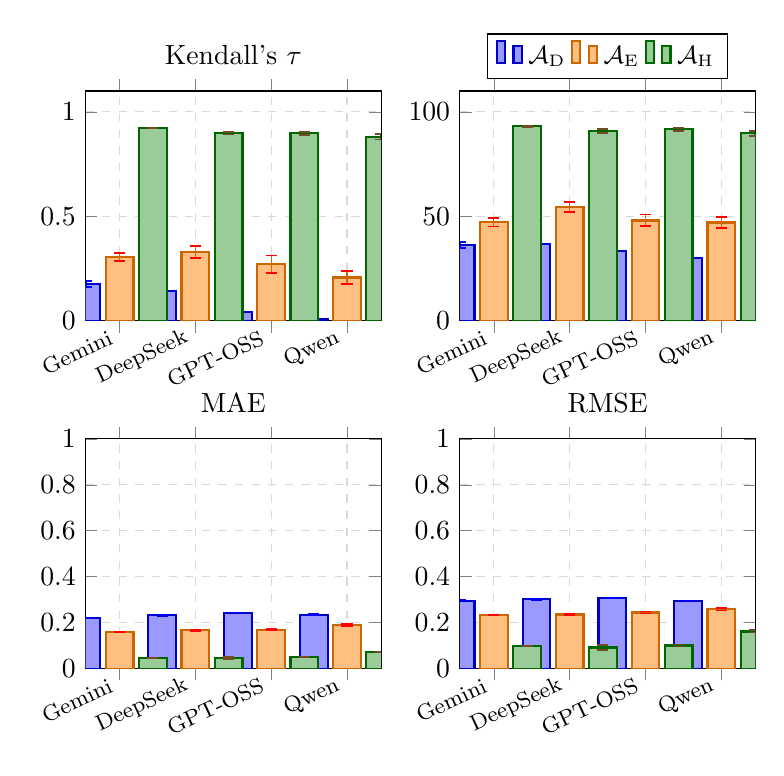
\begin{tikzpicture}
\begin{groupplot}[
    group style={
        group size=2 by 2,
        horizontal sep=1.0cm,
        vertical sep=1.5cm
    },
    width=0.44\columnwidth,
    height=4.5cm,
    ybar,
    enlarge x limits=0.15,
    symbolic x coords={Gemini, DeepSeek, GPT-OSS, Qwen},
    xtick=data,
    x tick label style={rotate=25, anchor=east, font=\footnotesize},
    grid=major,
    grid style={dashed, gray!30},
    error bars/y dir=both,
    error bars/y explicit,
    error bars/error mark options={
        rotate=90,
        line width=0.6pt,
        mark size=2pt
    }
]

\nextgroupplot[title={Kendall's $\tau$}, ymin=0, ymax=1.1]
\addplot+[fill=blue!40, draw=blue!80!black, thick] coordinates {
    (Gemini, 0.176) +- (0, 0.014) (DeepSeek, 0.144) +- (0, 0.041)
    (GPT-OSS, 0.041) +- (0, 0.045) (Qwen, 0.010) +- (0, 0.039)
};
\addplot+[fill=orange!50, draw=orange!80!black, thick] coordinates {
    (Gemini, 0.305) +- (0, 0.019) (DeepSeek, 0.328) +- (0, 0.029)
    (GPT-OSS, 0.270) +- (0, 0.042) (Qwen, 0.207) +- (0, 0.030)
};
\addplot+[fill=green!50!black!40, draw=green!40!black, thick] coordinates {
    (Gemini, 0.923) +- (0, 0.002) (DeepSeek, 0.897) +- (0, 0.005)
    (GPT-OSS, 0.897) +- (0, 0.007) (Qwen, 0.880) +- (0, 0.013)
};

\nextgroupplot[
    title={Top-1 (\%)}, ymin=0, ymax=110,
    legend style={font=\small, at={(0.5,1.05)}, anchor=south, legend columns=4}
]
\addplot+[fill=blue!40, draw=blue!80!black, thick] coordinates {
    (Gemini, 36.2) +- (0, 1.5) (DeepSeek, 36.7) +- (0, 3.1)
    (GPT-OSS, 33.3) +- (0, 2.4) (Qwen, 30.0) +- (0, 3.0)
};
\addplot+[fill=orange!50, draw=orange!80!black, thick] coordinates {
    (Gemini, 47.2) +- (0, 2.1) (DeepSeek, 54.5) +- (0, 2.3)
    (GPT-OSS, 48.0) +- (0, 2.8) (Qwen, 47.0) +- (0, 2.7)
};
\addplot+[fill=green!50!black!40, draw=green!40!black, thick] coordinates {
    (Gemini, 93.1) +- (0, 0.3) (DeepSeek, 90.8) +- (0, 0.9)
    (GPT-OSS, 91.6) +- (0, 0.8) (Qwen, 89.7) +- (0, 1.2)
};
\legend{$\mathcal{A}_{\text{D}}$, $\mathcal{A}_{\text{E}}$, $\mathcal{A}_{\text{H}}$}

\nextgroupplot[title={MAE}, ymin=0, ymax=1.0]
\addplot+[fill=blue!40, draw=blue!80!black, thick] coordinates {
    (Gemini, 0.220) +- (0, 0.002) (DeepSeek, 0.232) +- (0, 0.003)
    (GPT-OSS, 0.242) +- (0, 0.002) (Qwen, 0.235) +- (0, 0.002)
};
\addplot+[fill=orange!50, draw=orange!80!black, thick] coordinates {
    (Gemini, 0.159) +- (0, 0.001) (DeepSeek, 0.167) +- (0, 0.002)
    (GPT-OSS, 0.169) +- (0, 0.003) (Qwen, 0.191) +- (0, 0.004)
};
\addplot+[fill=green!50!black!40, draw=green!40!black, thick] coordinates {
    (Gemini, 0.048) +- (0, 0.001) (DeepSeek, 0.047) +- (0, 0.004)
    (GPT-OSS, 0.052) +- (0, 0.001) (Qwen, 0.072) +- (0, 0.002)
};

\nextgroupplot[title={RMSE}, ymin=0, ymax=1.0]
\addplot+[fill=blue!40, draw=blue!80!black, thick] coordinates {
    (Gemini, 0.296) +- (0, 0.002) (DeepSeek, 0.302) +- (0, 0.003)
    (GPT-OSS, 0.307) +- (0, 0.002) (Qwen, 0.295) +- (0, 0.002)
};
\addplot+[fill=orange!50, draw=orange!80!black, thick] coordinates {
    (Gemini, 0.233) +- (0, 0.001) (DeepSeek, 0.236) +- (0, 0.002)
    (GPT-OSS, 0.244) +- (0, 0.004) (Qwen, 0.259) +- (0, 0.006)
};
\addplot+[fill=green!50!black!40, draw=green!40!black, thick] coordinates {
    (Gemini, 0.100) +- (0, 0.001) (DeepSeek, 0.092) +- (0, 0.011)
    (GPT-OSS, 0.101) +- (0, 0.004) (Qwen, 0.162) +- (0, 0.005)
};

\end{groupplot}
\end{tikzpicture}
\caption{Overall performance by model (5-run mean $\pm$ std, 195 scenarios). Error bars show $\pm 1$ std across five runs.}
\label{fig:grouped_bars}
\end{figure}
\FloatBarrier

Figure~\ref{fig:grouped_bars} shows the architecture ordering is as expected. $\mathcal{A}_{\text{H}}$ dominates on every metric for all four models ($\tau > 0.88$, Top-1 $> 89\%$), $\mathcal{A}_{\text{E}}$ places second ($\tau \sim 0.2$--0.33), and $\mathcal{A}_{\text{D}}$ ranks third ($\tau$ near zero). Full per-model results by decision type appear in Appendix~\ref{app:per_model_results}; numerical values in Appendix~\ref{app:numerical_results}. The model success order is consistent across architectures, but the gap between models is smaller for $\mathcal{A}_{\text{H}}$ (cost implications discussed in Section~\ref{sec:res-efficiency}).

Ranking metrics partly reflect a structural advantage of $\mathcal{A}_{\text{H}}$: the LLM estimates scenario-level parameters, while the calculator parses and scores the three alternatives deterministically. Because many extraction errors shift all alternatives together, they largely cancel in the ranking; MAE/RMSE and parameter-specific failure patterns therefore provide the stronger evidence of extraction fidelity. Additionally, the calculator having the correct formulas and methods from the beginning also increases base scores. 

The ordering holds across all nine weight perturbations (Section~\ref{sec:mavt-design}). Pairwise differences between architectures are significant under Wilcoxon signed-rank testing (Stouffer-combined $p < 0.001$ for each adjacent pair on all metrics; full results in Appendix~\ref{app:significance}).

ICC(2,1) (two-way random, single-measures, absolute agreement) for MAE is 0.80--0.83 across architectures: model choice drives most score-level error. ICC for Top-1 is 0.08--0.27: scenario difficulty drives correct-alternative identification. Cliff's $\delta$ between $\mathcal{A}_{\text{E}}$ and $\mathcal{A}_{\text{H}}$ is large across all models on both MAE and $\tau$, and bootstrap 95\% BCa intervals for $\mathcal{A}_{\text{H}}$ show no overlap with $\mathcal{A}_{\text{E}}$ or $\mathcal{A}_{\text{D}}$ on any metric (Table~\ref{tab:bootstrap_ci}). These three analyses converge on the same conclusion: $\mathcal{A}_{\text{H}}$'s advantage is driven by architecture, not model choice or random variation.

Score-level error and ranking outcome tell the same story from opposite ends. $\mathcal{A}_{\text{D}}$ individual scores routinely miss by more than 0.2 points and offer no actionable ranking information: it performs only marginally above random overall ($\tau = 0.093$, Top-1 $= 34.1\%$ against a $33.3\%$ chance baseline) and below random in 8 of the 12 model--decision-type combinations. $\mathcal{A}_{\text{E}}$'s score error falls between the other two architectures, usable for rough ranking but not reliable score comparison, and its ranking signal is correspondingly weak but non-random: better than chance but unreliable for any single decision. $\mathcal{A}_{\text{H}}$ predictions deviate by only 5--7\% on average (its RMSE/MAE ratio is the highest of the three architectures because a small number of shower scenarios requiring GPM estimation produce larger deviations), and this low score error translates into near-perfect ranking across all models, identifying the correct order in nearly every scenario and the best option nine times out of ten at the Top-1 level.

\FloatBarrier
\subsection{Baseline Comparison}
\label{sec:res-baselines}
Table~\ref{tab:incremental-contribution} extends the comparison beyond the three LLM architectures to two non-LLM baselines, all evaluated on the same 195-scenario test set. Metrics are reported as per-type arithmetic means (averaging HVAC, Appliance, and Shower results equally) so that each decision type contributes equally regardless of scenario count; this prevents FixedDefault's strong HVAC performance from inflating its aggregate score. The Fixed-Default baseline substitutes fixed engineering defaults (68\textdegree{}F setpoint for HVAC, 7PM schedule for appliances, 8-minute shower duration) into the same physics calculators used by the ground truth.

\begin{table}[htbp]
\begin{threeparttable}
  \centering
  \textbf{Incremental contribution over Fixed-Default baseline}
  \caption{Per-type arithmetic means of Top-1 accuracy and Kendall's~$\tau$. Best and worst model shown for LLM architectures.}
  \label{tab:incremental-contribution}
  \begin{tabular}{lcccc}
    \toprule
    System & Top-1 & $\Delta$ vs FixedDef & Kendall $\tau$ & $\Delta$ vs FixedDef \\
    \midrule
    FixedDefault & 0.7282 & $0.0000$ & 0.6137 & $0.0000$ \\
    NearestNeighbor & 0.5692 & $-0.1590$ & 0.3709 & $-0.2428$ \\
    \addlinespace
    $\mathcal{A}_{\text{D}}$ (best: Gemini) & 0.371 & $-0.357$ & 0.193 & $-0.421$ \\
    $\mathcal{A}_{\text{D}}$ (worst: Qwen)   & 0.301 & $-0.428$ & 0.012 & $-0.602$ \\
    \addlinespace
    $\mathcal{A}_{\text{E}}$ (best: DeepSeek) & 0.552 & $-0.176$ & 0.341 & $-0.272$ \\
    $\mathcal{A}_{\text{E}}$ (worst: Qwen)    & 0.472 & $-0.257$ & 0.209 & $-0.405$ \\
    \addlinespace
    $\mathcal{A}_{\text{H}}$ (best: Gemini) & 0.928 & $+0.200$ & 0.920 & $+0.306$ \\
    $\mathcal{A}_{\text{H}}$ (worst: Qwen)  & 0.898 & $+0.169$ & 0.879 & $+0.266$ \\
    \bottomrule
  \end{tabular}
\end{threeparttable}
\end{table}
\FloatBarrier

FixedDefault achieves high HVAC accuracy (the 68\textdegree{}F setpoint is near-optimal for most Pennsylvania scenarios) and strong Shower ranking ($\tau = 0.800$, because the 8-minute/2.5-GPM default is near-optimal for most scenarios), but collapses on Appliance ($\tau = 0.097$), yielding a per-type average of $\tau = 0.610$. NearestNeighbor ($k=3$ majority vote over the RAG corpus) averages $\tau = 0.386$ across types, placing it between $\mathcal{A}_{\text{D}}$ and $\mathcal{A}_{\text{E}}$; unmodified exemplar copying provides partial but limited ranking signal.

This baseline is important because it shows that the benchmark is not merely rewarding calculator use. A fixed physics-based heuristic can perform well where its default happens to match the domain, but it does not adapt reliably across decision types. The LLM architectures must demonstrate flexible reasoning, not just calculator access, to outperform a fixed default.

\FloatBarrier
\subsection{Criterion-Level Error}
\label{sec:res-error}
\begin{figure*}[htbp]
\begin{threeparttable}
	\centering
	\plotCriterionMAEByModel
	\caption{MAE by criterion and model (5-run mean, 195 scenarios each). Each line is one model; the x-axis is architecture ($\mathcal{A}_{\text{D}}$~$\rightarrow$~$\mathcal{A}_{\text{E}}$~$\rightarrow$~$\mathcal{A}_{\text{H}}$).}
\end{threeparttable}
\label{fig:mae_criterion}
\end{figure*}

Figure~\ref{fig:mae_criterion} breaks MAE down by criterion and model (full numerical values in Appendix Table~\ref{tab:item6}). $\mathcal{A}_{\text{H}}$ achieves near-zero error on Comfort and Practicality across all four models. Again, this is expected: the calculator handles both criteria deterministically, with the LLM only estimating scenario-level parameters (occupancy, tank size) that shift all three alternatives together.

Error concentrates on Energy Cost and Environmental Impact for all three architectures. Even $\mathcal{A}_{\text{H}}$'s weakest model outperforms the best models of $\mathcal{A}_{\text{D}}$ and $\mathcal{A}_{\text{E}}$ on these criteria. The Environmental--Energy Cost gap persists across architectures. Shower environmental impact is measured in gallons of water while HVAC and Appliance environmental impact are measured in lbs\,CO\textsubscript{2}, so the pooled environmental MAE should not be read as error in a single physical unit.

\FloatBarrier
\subsection{Extraction Accuracy and Error Propagation}
\label{sec:res-extraction}
Score-level error measures how well $\mathcal{A}_{\text{H}}$ reproduces the reference calculator's output, but it does not separate two distinct questions: how accurately the LLM estimates each withheld engineering parameter, and whether an estimation error changes the recommendation. Table~\ref{tab:extraction_accuracy} reports both. Extracted parameters were compared against the scenario source values for all 195 test scenarios, and a counterfactual analysis re-ran the calculator with each erroneous parameter substituted individually, holding all others at their true values, to measure how often the top-ranked alternative changes.

Absolute extraction error is substantial. HVAC equipment age is estimated to within 6.1--8.5 years on average and shower tank size to within 6.7--8.9 gallons, both large fractions of the plausible range. Categorical extraction is more reliable: appliance type and baseline run time are recovered essentially perfectly, while HVAC occupancy context reaches only 75--81\%.

That error rarely propagates to the decision. For most parameters the conditional probability that an extraction error flips the top-ranked alternative sits below 0.09, and for HVAC equipment age it is zero across all four models. The reason is structural: the LLM estimates scenario-level parameters that enter all three alternatives identically, so an error shifts the whole choice set and largely cancels in the ranking. Shower GPM is the consistent exception, carrying the highest flip probability for every model (0.133--0.233), two to three times the next-largest parameter. GPM is the one extracted parameter that must map a discrete homeowner-facing tier (low\_flow, standard, high\_flow) onto a continuous value that scales both energy and water volume directly, and it is the parameter behind the Shower results being $\mathcal{A}_{\text{H}}$'s weakest decision type (Section~\ref{sec:res-bytype}). This localizes the error-cancellation mechanism rather than assuming it: ranking robustness is real, but it rests on common-mode error, and it weakens precisely where a parameter is both decision-critical and recovered from a coarse proxy.

\begin{table*}[htbp]
\begin{threeparttable}
\footnotesize
\centering
\textbf{Extraction accuracy and counterfactual top-1 sensitivity}
\renewcommand{\arraystretch}{1.15}
\begin{tabular}{llcccccccc}
\toprule
 & & \multicolumn{4}{c}{MAE} & \multicolumn{4}{c}{$P(\text{top-1 change} \mid \text{error})$} \\
\cmidrule(lr){3-6}\cmidrule(lr){7-10}
Type & Parameter & GPT-OSS & Qwen & DeepSeek & Gemini & GPT-OSS & Qwen & DeepSeek & Gemini \\
\midrule
HVAC & R-value & 3.594 & 3.699 & 2.312 & 1.766 & 0.015 & 0.086 & 0.015 & 0.000 \\
HVAC & SEER & 2.135 & 1.585 & 1.602 & 1.313 & 0.049 & 0.033 & 0.032 & 0.075 \\
HVAC & HVAC age (yr) & 8.455 & 6.105 & 8.462 & 7.640 & 0.000 & 0.000 & 0.000 & 0.000 \\
Appliance & kWh/cycle & 0.425 & 0.975 & 0.341 & 0.541 & 0.016 & 0.066 & 0.016 & 0.031 \\
Shower & GPM & 0.256 & 0.271 & 0.368 & 0.367 & \textbf{0.152} & \textbf{0.133} & \textbf{0.185} & \textbf{0.233} \\
Shower & Tank size (gal) & 8.100 & 8.933 & 6.933 & 6.733 & 0.000 & 0.026 & 0.025 & 0.000 \\
Shower & Heater setpoint (\textdegree{}F) & 4.717 & 4.583 & 8.317 & 4.583 & 0.042 & 0.050 & 0.062 & 0.050 \\
\bottomrule
\end{tabular}
\renewcommand{\arraystretch}{1.0}
\begin{tablenotes}
\item Numeric parameters only; all 195 test scenarios matched for every model. Categorical accuracy: appliance type 100\% (GPT-OSS, Qwen, DeepSeek) and 93.8\% (Gemini); baseline time 100\% for all models; HVAC occupancy context 75.4\%, 78.6\%, 81.4\%, and 80.0\% respectively. Counterfactual probabilities are conditional on the parameter being mis-estimated, with each parameter varied individually.
\end{tablenotes}
\caption{Per-parameter extraction error and the probability that an extraction error changes the top-ranked alternative.}
\label{tab:extraction_accuracy}
\end{threeparttable}
\end{table*}

\FloatBarrier
\subsection{Isolating the Contribution of Extraction}
\label{sec:res-paramprov}
The error-cancellation mechanism in Section~\ref{sec:res-extraction} raises a sharper objection: if extraction errors largely cancel in the ranking, perhaps $\mathcal{A}_{\text{H}}$ ranks well simply because it has access to the reference calculator, and the LLM's parameter estimates contribute little. A parameter-provenance ablation separates the two (design and significance-testing methodology in Section~\ref{sec:hybrid-ablation-methods}). Three arms are scored by the same calculators over the same 195 test scenarios, differing only in where the withheld engineering parameters come from: the scenario's true values, the values the LLM actually returned, and a single corpus-median constant per parameter reused for every scenario. The first arm is the reference ranking itself and so is the ceiling; the third performs no per-scenario inference at all and so isolates what calculator access alone buys. Table~\ref{tab:param_provenance} reports the result.

Calculator access alone is not sufficient. With no per-scenario inference, the median-parameter arm reaches $\tau = 0.641$ and Top-1 of 76.9\%, well above chance but far below the published $\mathcal{A}_{\text{H}}$ results. LLM extraction lifts this to $\tau = 0.897$--$0.921$ and Top-1 of 91.3--94.3\%, a gain of roughly 0.26 in $\tau$ attributable to extraction rather than to the calculator. The extracted arm's $\tau$ falls within 0.02 of the main-text $\mathcal{A}_{\text{H}}$ values in Figure~\ref{fig:grouped_bars} for every model, which validates the ablation harness against known results. The remaining gap to the ceiling, about 0.08--0.10 in $\tau$, is the headroom a better estimator could recover. Extraction is therefore doing substantive work: the common-mode cancellation identified above acts on informative estimates, not on noise.

\begin{table}[htbp]
\begin{threeparttable}
\footnotesize
\centering
\textbf{Parameter-provenance ablation}
\renewcommand{\arraystretch}{1.15}
\begin{tabular}{llccc}
\toprule
Model & Parameter source & $\tau$ & Top-1 & MAE \\
\midrule
GPT-OSS & True (ceiling) & 1.000 & 1.000 & 0.000 \\
GPT-OSS & LLM-extracted & 0.921 & 0.943 & 0.046 \\
GPT-OSS & Corpus median & 0.641 & 0.769 & 0.122 \\
\midrule
Qwen & True (ceiling) & 1.000 & 1.000 & 0.000 \\
Qwen & LLM-extracted & 0.897 & 0.913 & 0.066 \\
Qwen & Corpus median & 0.641 & 0.769 & 0.122 \\
\midrule
DeepSeek & True (ceiling) & 1.000 & 1.000 & 0.000 \\
DeepSeek & LLM-extracted & 0.904 & 0.913 & 0.041 \\
DeepSeek & Corpus median & 0.641 & 0.769 & 0.122 \\
\bottomrule
\end{tabular}
\renewcommand{\arraystretch}{1.0}
\begin{tablenotes}
\item All arms scored by the same reference calculators over the same 195 test scenarios; the arms differ only in the source of the withheld engineering parameters. The true-parameter arm reproduces the reference ranking exactly by construction, which serves as a correctness check on the harness. The corpus-median arm uses one constant per parameter and no model output, so it is identical across models. Scenarios whose extraction failed are excluded from that arm rather than defaulted; the extracted arm scored 194 of 195 scenarios for GPT-OSS and 195 for the other two models.
\end{tablenotes}
\caption{Ranking accuracy of $\mathcal{A}_{\text{H}}$ with true, LLM-extracted, and corpus-median hidden parameters.}
\label{tab:param_provenance}
\end{threeparttable}
\end{table}

Friedman tests confirm the three arms differ by more than run-to-run noise for every model on every metric ($\chi^2_2$ ranging from 52.5 to 305.3, all $p_{\text{Holm}} < 10^{-11}$ across the nine-test family described in Section~\ref{sec:hybrid-ablation-methods}). Post-hoc Wilcoxon signed-rank tests isolate where that difference sits. Extracted beats default\_params on Kendall's $\tau$ for all three models ($p_{\text{Holm}} < 10^{-6}$, Cliff's $\delta$ between $-0.22$ and $-0.23$, small) and on MAE ($p_{\text{Holm}} < 10^{-10}$, $\delta$ between 0.35 and 0.48, medium to large); the Top-1 comparison is significant for all three models but the effect size is small for GPT-OSS ($\delta=-0.175$) and negligible for DeepSeek and Qwen ($\delta=-0.144$), since Top-1 is coarser than $\tau$ and both arms already place the correct alternative first most of the time.

The remaining gap to the ceiling tells a different story. Extracted differs from true\_params significantly on all three metrics for all three models, but on Kendall's $\tau$ and Top-1 the effect size is negligible for every model ($|\delta| \leq 0.118$); only on MAE is the gap large ($\delta > 0.88$ for all three models). With $n=195$ paired scenarios, a small and consistent shortfall is enough to reach significance without being practically large. Extraction has closed nearly all of the ranking gap to the ceiling; what remains is a score-calibration gap, consistent with the RMSE/MAE discussion in Section~\ref{sec:res-error}.

This comparison is hard to dismiss as an artifact. Every arm is scored by the same calculator code used for the ground truth and by $\mathcal{A}_{\text{H}}$ itself, so the arms differ only in one input, not in scoring logic; the ablation draws on data already collected for the main benchmark rather than a new run assembled for this comparison, and reproduces the published $\mathcal{A}_{\text{H}}$ numbers almost exactly when scored with extracted parameters; and the significance pipeline reuses the same reviewed Friedman/Holm/Cliff's-$\delta$ code as the RAG and prompt ablations (Sections~\ref{sec:rag-ablation-methods}, \ref{sec:prompt-ablation-methods}).

This ablation answers the objection raised in Section~\ref{sec:res-extraction}: as shown above, $\mathcal{A}_{\text{H}}$'s advantage over $\mathcal{A}_{\text{D}}$ and $\mathcal{A}_{\text{E}}$ is not simply that it has a calculator, since extraction accounts for most of the gap between the median-parameter arm and full performance. Parameter extraction and deterministic scoring are both doing real work, and neither one alone would suffice.

\FloatBarrier
\subsection{Performance by Decision Type}
\label{sec:res-bytype}
Table~\ref{tab:item7} reports $\tau$ by decision type; per-decision-type breakdowns for both Kendall's $\tau$ and Top-1 accuracy appear in Appendix~\ref{app:decision_type_full_figures}. $\mathcal{A}_{\text{H}}$ excels across all three decision types for every model. Shower is the weakest due to GPM estimation limits, still far above the other architectures.

\begin{table*}[t]
\begin{threeparttable}
\footnotesize
\centering
\textbf{Ranking accuracy by decision type}
\renewcommand{\arraystretch}{1.15}
\begin{tabular}{lcccccc}
\toprule
 & \multicolumn{2}{c}{$\mathcal{A}_{\text{D}}$} & \multicolumn{2}{c}{$\mathcal{A}_{\text{E}}$} & \multicolumn{2}{c}{$\mathcal{A}_{\text{H}}$} \\
\cmidrule(lr){2-3}\cmidrule(lr){4-5}\cmidrule(lr){6-7}
Decision Type & $\tau$ & Top-1 (\%) & $\tau$ & Top-1 (\%) & $\tau$ & Top-1 (\%) \\
\midrule
HVAC & & & & & & \\
\quad Best & 0.135 (O) & 39.7 (O) & 0.265 (O) & 46.9 (O) & \textbf{0.977 (G)} & \textbf{96.6 (G)} \\
\quad Worst & $-0.102$ (D) & 19.8 (D) & $-0.116$ (G) & 15.3 (G) & \textbf{0.881 (Q)} & \textbf{87.4 (Q)} \\
Appliance & & & & & & \\
\quad Best & 0.029 (D) & 31.7 (D) & 0.417 (D) & 70.2 (D) & \textbf{0.975 (D)} & \textbf{98.5 (D)} \\
\quad Worst & $-0.147$ (O) & 26.8 (O) & $-0.048$ (O) & 30.5 (O) & \textbf{0.906 (Q)} & \textbf{92.9 (Q)} \\
Shower & & & & & & \\
\quad Best & 0.633 (G) & 61.0 (G) & 0.766 (G) & 75.5 (G) & \textbf{0.851 (Q)} & \textbf{89.0 (Q)} \\
\quad Worst & 0.069 (Q) & 34.3 (Q) & 0.236 (Q) & 48.3 (Q) & \textbf{0.784 (O)} & \textbf{82.0 (O)} \\
\bottomrule
\end{tabular}
\renewcommand{\arraystretch}{1.0}
\caption{5-run per-run-then-average, showing best and worst model per cell (G = Gemini, D = DeepSeek, O = GPT-OSS, Q = Qwen). Per-model results by decision type appear in Appendix~\ref{app:per_model_results}.}
\label{tab:item7}
\end{threeparttable}
\end{table*}

$\mathcal{A}_{\text{E}}$ shows wide model-level variance on HVAC, ranging from a positive signal to below zero. On Appliance, performance splits similarly. Shower is $\mathcal{A}_{\text{E}}$'s strongest type across all models. Shower scoring depends primarily on duration and flow rate---fewer interacting variables than HVAC load calculations or appliance TOU scheduling---so the exemplar's calibration anchor is more effective here.

The ordering $\mathcal{A}_{\text{H}} > \mathcal{A}_{\text{E}} > \mathcal{A}_{\text{D}}$ is consistent across all three types, but the margin varies with task dimensionality. HVAC---the highest-dimensional task (insulation, SEER, age, occupancy, square footage, outdoor temperature)---shows the widest gap between $\mathcal{A}_{\text{H}}$ and $\mathcal{A}_{\text{E}}$ because correct ranking requires accurate joint estimation of multiple parameters. Shower---the lowest-dimensional (duration, flow rate, tank size)---shows the narrowest gap because a single well-estimated parameter can carry the ranking. Appliance results for $\mathcal{A}_{\text{H}}$ track extraction quality since the baseline time parameter varies across alternatives, making it the strongest test of extraction fidelity.

$\mathcal{A}_{\text{D}}$ is near-random or below on HVAC and Appliance for all models. Shower diverges: the two strongest models show meaningful positive correlation while the two weakest remain near-random, likely because shower scoring depends primarily on duration and flow rate, which are easier to read from scenario text than HVAC load calculations or appliance TOU scheduling.

\FloatBarrier
\subsection{Sensitivity Analysis}
\label{sec:res-sensitivity}

To test the stability of the ranking results, weights were perturbed by $\pm 0.05$ on each of the four criteria individually, redistributing the difference equally across the remaining three, plus one equal-weight scenario ($w_j = 0.25$ for all $j$).

\begin{table}[htbp]
\begin{threeparttable}
\small
\centering
\textbf{Sensitivity analysis: mean ranking outcomes under weight perturbation}
\renewcommand{\arraystretch}{1.15}
\begin{tabular}{@{} l ccc @{}}
\toprule
\textbf{Perturbation} & $\mathcal{A}_{\text{D}}$ & $\mathcal{A}_{\text{E}}$ & $\mathcal{A}_{\text{H}}$ \\
\midrule
Baseline    & 0.093 & 0.278 & 0.899 \\
Ene $+0.05$ & 0.131 & 0.341 & 0.891 \\
Ene $-0.05$ & 0.101 & 0.362 & 0.928 \\
Env $+0.05$ & 0.106 & 0.341 & 0.904 \\
Env $-0.05$ & 0.109 & 0.341 & 0.928 \\
Com $+0.05$ & 0.100 & 0.357 & 0.918 \\
Com $-0.05$ & 0.140 & 0.320 & 0.867 \\
Pra $+0.05$ & 0.101 & 0.334 & 0.917 \\
Pra $-0.05$ & 0.113 & 0.361 & 0.907 \\
Equal       & 0.139 & 0.368 & 0.913 \\
\bottomrule
\end{tabular}
\renewcommand{\arraystretch}{1.0}
\begin{tablenotes}
\item Each cell is the arithmetic mean of the four per-model Kendall's $\tau$ values reported in Appendix Tables~\ref{tab:sensitivity_gemini} and~\ref{tab:sensitivity_gptoss}, not a scenario-pooled statistic. Perturbation vectors are defined in Table~\ref{tab:sensitivity_weights} (Appendix~\ref{app:sensitivity_full}).
\end{tablenotes}
\caption{Mean Kendall's $\tau$ across the four evaluated models (Gemini, DeepSeek, GPT-OSS, Qwen), by architecture and weight-perturbation scenario.}
\label{tab:sensitivity_pooled}
\end{threeparttable}
\end{table}

Table~\ref{tab:sensitivity_pooled} reports the mean Kendall's $\tau$ across the four evaluated models for each of the nine weight-perturbation scenarios plus baseline and equal weights. The architecture ordering $\mathcal{A}_{\text{H}} > \mathcal{A}_{\text{E}} > \mathcal{A}_{\text{D}}$ holds for every perturbation, with no overlap between architecture groups: the highest $\mathcal{A}_{\text{D}}$ mean (0.140) sits below the lowest $\mathcal{A}_{\text{E}}$ mean (0.278), which in turn sits below the lowest $\mathcal{A}_{\text{H}}$ mean (0.867). No model--weight combination allows a weaker architecture to match a stronger one; per-model results appear in Appendix~\ref{app:sensitivity_full}.

\FloatBarrier
\subsection{RAG Ablation}
\label{sec:rag-ablation}
\begin{figure}[htbp]
	\centering
	\plotRagAblation
	\caption{RAG ablation results: Kendall's $\tau$ by configuration and model on the full 90-scenario RAG corpus. Configurations are ordered by overall $\tau$. Dashed line marks $\tau = 0$.}
\label{fig:rag_ablation}
\end{figure}

Figure~\ref{fig:rag_ablation} summarizes a RAG ablation study conducted on the full 90-scenario RAG corpus with seven configurations across three models, plus an offline nearest-neighbor baseline. Gemini is excluded from the ablation matrix because its output pricing is roughly fifty times that of the other models. Unlike the corpus-level \texttt{NearestNeighbor} baseline in Section~\ref{sec:res-baselines} ($k=3$ majority vote, evaluated on the 195-scenario test set), this offline baseline performs leave-one-out retrieval within the 90-scenario RAG corpus itself and assigns the retrieved scenario's score directly without LLM rescoring or voting, yielding $\tau = 0.001$ (95\% CI: $[-0.175,\, 0.172]$), indistinguishable from zero and confirming that naive exemplar copying provides no ranking signal. The full per-configuration table underlying Figure~\ref{fig:rag_ablation} appears in Appendix~\ref{app:rag_ablation_full}.

Exemplar content matters; retrieval depth does not. The strongest cluster of configurations---exemplars\_no\_hidden\_params, the $k=3$ control, $k=1$, $k=5$, and the alternate embedding model---are statistically indistinguishable from one another (full per-configuration values in Appendix~\ref{app:rag_ablation_full} and Figure~\ref{fig:rag_ablation}). That exemplars\_no\_hidden\_params matches the control indicates the engineering parameters (R-value, SEER, GPM, kWh/cycle) contribute little additional signal, since the model infers what it needs from the surrounding context; that $k=1$ and $k=5$ both match the control means the number of retrieved exemplars does not drive performance within this range. The alternate embedding model (paraphrase-MiniLM-L3-v2) is a lightweight model with limited semantic resolution, so its matching the control suggests the anchoring effect of exemplar scores is robust to embedder quality, though stronger embedders might yield additional gains. The two weakest configurations fail for different reasons. The descriptions\_no\_scores\_ranks configuration, which omits all quantitative scores from the retrieved exemplars, drops well below the other LLM-based configurations: without scores, the exemplar provides a worked example of the scoring task but no calibration anchor, so the model must generate scores from scratch and the exemplar contributes little beyond framing. The random-exemplar variant is likewise far below the top cluster, because semantic retrieval selects exemplars that share the same decision type and parameter ranges, making them genuinely useful guides, while random draws may come from a different decision domain and lack relevance even when they happen to share a decision type.

A Friedman test across configurations, Holm-corrected across this four-metric family, is not significant on Kendall's $\tau$ ($\chi^2_7 = 9.90$, $p = 0.195$, $p_{\text{Holm}} = 0.389$) or Top-1 accuracy ($\chi^2_7 = 8.67$, $p = 0.277$, $p_{\text{Holm}} = 0.277$), and is significant on MAE ($\chi^2_7 = 79.97$, $p < 0.001$, $p_{\text{Holm}} < 0.001$) and RMSE ($\chi^2_7 = 79.00$, $p < 0.001$, $p_{\text{Holm}} < 0.001$). Post-hoc Wilcoxon signed-rank tests, run only for the two metrics whose Holm-corrected omnibus is significant and Holm-corrected again within their own pairwise family, confirm that the control, retrieval, exemplar-content, and alternate-embedding configurations form a statistically indistinguishable cluster, while random exemplars and descriptions without scores are significantly worse than every configuration in the top cluster, with small to medium Cliff's $\delta$. The scale of the difference is what separates the two groups: the top cluster holds MAE near 0.09--0.10, while descriptions without scores (0.147) and random exemplars (0.144) approach half again the error. That the $\tau$ omnibus is not significant while the error-magnitude omnibus is decisively so indicates the exemplar-content manipulations shift how well the model calibrates the absolute scores more than the order it places the three alternatives in. 

No pair of retrieval counts separates on either $\tau$ or MAE (all $p_{\text{Holm}} > 0.62$, Cliff's $\delta$ negligible), so retrieval depth is not a meaningful design lever within the range tested. Cost then decides: $k=5$ appends four additional exemplars to each prompt (${\approx}857$ tokens per exemplar, $+3{,}428$ tokens per call), approximately doubling the input-token cost relative to $k=1$. Given the statistical equivalence, $k=1$ is the recommended production setting.

\FloatBarrier
\subsection{Prompt Sensitivity}
\label{sec:prompt-ablation}

A reviewer may reasonably ask whether the reported architecture ordering reflects the design of $\mathcal{A}_{\text{D}}$ and $\mathcal{A}_{\text{E}}$ or the particular prompts used to implement them. To separate the two, we re-ran both architectures under three controlled prompt perturbations across three models and five runs each: removing the numeric anchors from the scoring instructions (no\_anchors), adding an explicit chain-of-thought scaffold before the JSON response (cot\_scaffold), and rescaling the response range from 0--1 to 0--10 (scale\_0\_10). The full matrix comprises 105 cells and 20{,}475 scenario-level observations. $\mathcal{A}_{\text{E}}$ ships without numeric anchors, so no\_anchors has no $\mathcal{A}_{\text{E}}$ arm and those strata compare three variants rather than four. The harness re-declares the shipped prompts rather than importing them and asserts at startup that its control arm matches the deployed text, so a drift between the ablation and the production prompt fails loudly instead of silently weakening the baseline.

\begin{table}[htbp]
\begin{threeparttable}
\small
\centering
\textbf{Kendall's $\tau$ and Top-1 accuracy by prompt variant}
\renewcommand{\arraystretch}{1.15}
\begin{tabular}{llcccc}
\toprule
& & \multicolumn{4}{c}{Prompt variant} \\
\cmidrule(lr){3-6}
Arch. & Model & control & no\_anchors & cot\_scaffold & scale\_0\_10 \\
\midrule
\multicolumn{6}{l}{\emph{Kendall's $\tau$}} \\
$\mathcal{A}_{\text{D}}$ & DeepSeek & 0.129 & 0.147 & 0.161 & 0.167 \\
$\mathcal{A}_{\text{D}}$ & GPT-OSS  & 0.053 & 0.100 & 0.041 & $-$0.001 \\
$\mathcal{A}_{\text{D}}$ & Qwen     & $-$0.052 & 0.024 & 0.092 & 0.015 \\
$\mathcal{A}_{\text{E}}$ & DeepSeek & \textbf{0.304} & --- & 0.180 & 0.246 \\
$\mathcal{A}_{\text{E}}$ & GPT-OSS  & \textbf{0.262} & --- & 0.200 & 0.261 \\
$\mathcal{A}_{\text{E}}$ & Qwen     & \textbf{0.206} & --- & 0.194 & 0.102 \\
\midrule
\multicolumn{6}{l}{\emph{Top-1 accuracy}} \\
$\mathcal{A}_{\text{D}}$ & DeepSeek & 0.394 & 0.458 & 0.363 & 0.412 \\
$\mathcal{A}_{\text{D}}$ & GPT-OSS  & 0.344 & 0.368 & 0.328 & 0.320 \\
$\mathcal{A}_{\text{D}}$ & Qwen     & 0.289 & 0.371 & 0.333 & 0.329 \\
$\mathcal{A}_{\text{E}}$ & DeepSeek & \textbf{0.552} & --- & 0.367 & 0.478 \\
$\mathcal{A}_{\text{E}}$ & GPT-OSS  & 0.454 & --- & 0.440 & \textbf{0.489} \\
$\mathcal{A}_{\text{E}}$ & Qwen     & \textbf{0.474} & --- & 0.399 & 0.407 \\
\bottomrule
\end{tabular}
\renewcommand{\arraystretch}{1.0}
\begin{tablenotes}\footnotesize
\item Mean over five runs on 195 Test scenarios per cell, except $\mathcal{A}_{\text{D}}$ control and no\_anchors, which use ten runs: no\_anchors was extended from five to ten runs to give a borderline control-vs-no\_anchors comparison enough power to resolve, and control was matched to ten for a balanced comparison. Bold marks the best variant within each architecture--model row group. $\mathcal{A}_{\text{E}}$ has no no\_anchors arm because its shipped prompt contains no numeric anchors.
\end{tablenotes}
\caption{Prompt-sensitivity ablation. Within each model, every $\mathcal{A}_{\text{E}}$ configuration remains above every $\mathcal{A}_{\text{D}}$ configuration on Kendall's $\tau$, so no prompt perturbation reverses the architecture ordering for a fixed model.}
\label{tab:prompt_ablation}
\end{threeparttable}
\end{table}

Table~\ref{tab:prompt_ablation} shows the architecture ordering survives every perturbation when architecture and model are held together, though a weaker model running the stronger architecture can still trail a stronger model running the weaker one ($\mathcal{A}_{\text{E}}$ with Qwen falls to $\tau = 0.102$ under scale\_0\_10, below $\mathcal{A}_{\text{D}}$ with DeepSeek at $\tau = 0.167$), the same model--architecture interaction visible in the sensitivity analysis (Section~\ref{sec:res-sensitivity}). The shipped prompts are not an unlucky draw: of the pairwise comparisons that reach significance under the two-stage Holm correction (Section~\ref{sec:prompt-ablation-methods}), every one involving the control favors the control for $\mathcal{A}_{\text{E}}$, while the few significant $\mathcal{A}_{\text{D}}$ comparisons reflect that architecture operating near the noise floor; full statistics appear in Appendix~\ref{app:significance}. As in the RAG ablation (Section~\ref{sec:rag-ablation}), ranking is more stable under perturbation than calibration: the Friedman omnibus on Kendall's $\tau$ is not significant for any $\mathcal{A}_{\text{E}}$ model, while the Top-1 omnibus is significant for DeepSeek, so prompt wording shifts which alternative is ranked first more readily than it shifts the relative order of all three.

Two caveats bound this result. First, cot\_scaffold confounds reasoning with parsing: the scaffold moves the JSON payload behind free-form reasoning text, and the harness must fall back to extracting the last balanced object in the response. That arm records the lowest success rate in the matrix (0.961 for $\mathcal{A}_{\text{E}}$/GPT-OSS, against 1.000 for scale\_0\_10), so part of its measured penalty is extraction reliability rather than reasoning quality. Second, the three perturbations were applied one at a time rather than factorially, so these results speak to the effect of each manipulation in isolation and not to interactions between them.

\FloatBarrier
\subsection{Efficiency and Cost}
\label{sec:res-efficiency}

\begin{table}[htpb]
\begin{threeparttable}
\small
\centering
\textbf{Cost per run (USD) by model}
\renewcommand{\arraystretch}{1.15}
\begin{tabular}{lcccc}
\toprule
Architecture & Gemini & DeepSeek & GPT-OSS & Qwen \\
\midrule
$\mathcal{A}_{\text{D}}$ & \$0.802 & \$0.087 & \$0.023 & \$0.043 \\
$\mathcal{A}_{\text{E}}$ & \$1.024 & \$0.036 & \$0.023 & \$0.042 \\
$\mathcal{A}_{\text{H}}$ & \$0.280 & \$0.011 & \$0.006 & \$0.012 \\
\bottomrule
\end{tabular}
\renewcommand{\arraystretch}{1.0}
\caption{Cost per run (USD) by architecture and model, computed from measured per-run token counts priced at OpenRouter list rates.}
\label{tab:item8}
\end{threeparttable}
\end{table}

Table~\ref{tab:item8} reports API usage and costs based on OpenRouter pricing as of August 1, 2026, computed from the per-run token counts recorded in each run's diagnostics. $\mathcal{A}_{\text{H}}$ makes one API call per scenario versus three for $\mathcal{A}_{\text{D}}$ and $\mathcal{A}_{\text{E}}$, and its shorter prompts average 565--630 input+output tokens per scenario versus 2,124--3,424 for $\mathcal{A}_{\text{D}}$ and 1,971--2,474 for $\mathcal{A}_{\text{E}}$. Cost per 195-scenario run ranges from \$0.006 (GPT-OSS $\mathcal{A}_{\text{H}}$) to \$1.024 (Gemini $\mathcal{A}_{\text{E}}$). Against $\mathcal{A}_{\text{H}}$ on the same model, $\mathcal{A}_{\text{D}}$ costs 2.9--7.9$\times$ more and $\mathcal{A}_{\text{E}}$ 3.3--3.8$\times$ more, driven by the three-call-per-scenario structure and exemplar token overhead. The priciest configuration stays under \$1.05 per full evaluation. $\mathcal{A}_{\text{H}}$ compresses the capability gap, making cheaper models viable in production with minimal accuracy loss.

\FloatBarrier
\subsection{Failure Analysis}
\label{sec:res-failures}

To determine whether failures follow systematic patterns, we identified every scenario across all 60 runs (5 runs $\times$ 4 models $\times$ 3 architectures) that produced a sentinel score of 1928 (the reserved failure indicator) in any criterion. Table~\ref{tab:failure_arch_model} reports failure counts per architecture and model.

\begin{table}[htbp]
\small\centering
\caption{Failure counts per architecture and model (summed across 5 runs). Counts are unique scenario-run failures (one per scenario per run), not raw output rows.}
\label{tab:failure_arch_model}
\begin{tabular}{lccccc}
\toprule
Architecture & Gemini & DeepSeek & GPT-OSS & Qwen & Total \\
\midrule
$\mathcal{A}_{\text{D}}$ & 21 & 0 & 0 & 6 & 27 \\
$\mathcal{A}_{\text{E}}$ & 0 & 60 & 0 & 0 & 60 \\
$\mathcal{A}_{\text{H}}$ & 0 & 1 & 117 & 2 & 120 \\
\bottomrule
\end{tabular}
\end{table}

These counts reflect total scenario-run failures; unique scenario failures (deduplicated across runs) are lower, as cross-run recovery rescues many transient failures.

Because failed scenarios are excluded from their run's metric computation, every metric reported above is conditional on successful extraction. Weighting each architecture's conditional Kendall's $\tau$ by its success rate gives a failure-inclusive figure: $\mathcal{A}_{\text{H}}$ falls from 0.899 to 0.872, while $\mathcal{A}_{\text{E}}$ (0.277 to 0.276) and $\mathcal{A}_{\text{D}}$ (0.093 to 0.092) are essentially unchanged because both fail far less often. The one case where this matters is GPT-OSS on $\mathcal{A}_{\text{H}}$, whose 88.0\% success rate lowers its success-weighted $\tau$ from 0.897 to 0.789 and its Top-1 from 91.6\% to 80.6\%. The $\mathcal{A}_{\text{H}} > \mathcal{A}_{\text{E}} > \mathcal{A}_{\text{D}}$ ordering holds for all four models on the success-weighted metric, with the narrowest margin being GPT-OSS at 0.789 against 0.270 for $\mathcal{A}_{\text{E}}$.

GPT-OSS incurred the most extraction failures, concentrated in HVAC scenarios (as shown in Appendix~\ref{app:worked_example}). DeepSeek, Gemini, and Qwen exhibited near-zero failure rates on $\mathcal{A}_{\text{H}}$.

\begin{table}[htbp]
\small\centering
\caption{Nonzero-firing failure mode counts per architecture (5-run total across all models).\protect\footnotemark}
\label{tab:failure_modes}
\begin{tabular}{lccc}
\toprule
Mode & $\mathcal{A}_{\text{D}}$ & $\mathcal{A}_{\text{E}}$ & $\mathcal{A}_{\text{H}}$ \\
\midrule
\texttt{EXTRACTION\_INVALID\_JSON} & 27 & 60 & 0 \\
\texttt{FAILED\_EXTRACTION\_INVALID\_PARAMETERS} & 0 & 0 & 120 \\
\bottomrule
\end{tabular}
\footnotetext{Counts are 5-run totals summed across all four models. Of fifteen possible failure codes, only these two ever fired across all 60 runs; the remaining thirteen were checked and never triggered.}
\end{table}

The most common failure mode for $\mathcal{A}_{\text{D}}$ and $\mathcal{A}_{\text{E}}$ is \texttt{EXTRACTION\_INVALID\_JSON} (model returns unparseable output), while for $\mathcal{A}_{\text{H}}$, all failures concentrate in \texttt{FAILED\_EXTRACTION\_INVALID\_PARAMETERS} (extracted numeric parameter falls outside the physical validation bounds), driven almost entirely by GPT-OSS on HVAC scenarios.

Cross-run recovery eliminates most of these failures: when a scenario fails in one run but succeeds in another, the successful run's score is used. After cross-run matching, 0\% of scenarios remain unscored across all five runs, because cross-run recovery ensures at least one successful run per scenario. The "without recovery" values exclude scenarios where all five runs failed (equivalent to the primary per-run-then-average protocol), while "with recovery" uses cross-run success to score every scenario. Without cross-run recovery, pooled $\tau$ is 0.886 and Top-1 is 90.8\%, versus 0.897 and 91.6\% with recovery.



\FloatBarrier
\subsection{Run-to-Run Variance}
\label{sec:res-variance}
\begin{figure*}[htbp]
\begin{threeparttable}
\centering
\begin{minipage}{0.24\textwidth}
\centering
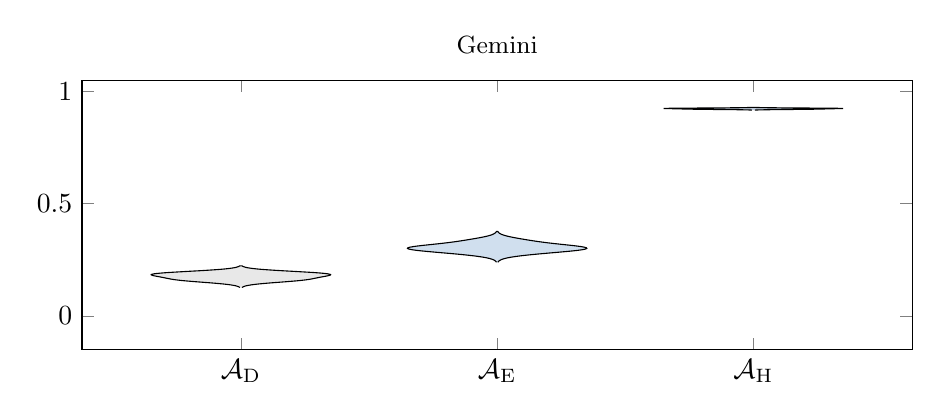
\begin{tikzpicture}
\begin{axis}[width=\textwidth, height=5cm, ymin=-0.15, ymax=1.05,
  xtick={1,2,3}, xticklabels={$\mathcal{A}_{\text{D}}$,$\mathcal{A}_{\text{E}}$,$\mathcal{A}_{\text{H}}$},
  title={\small Gemini}, title style={font=\small}]
\addplot[no marks, fill=colorPure!60, fill opacity=0.5] coordinates { (1.0043,0.1261) (1.0067,0.1281) (1.0100,0.1300) (1.0147,0.1320) (1.0210,0.1340) (1.0293,0.1359) (1.0398,0.1379) (1.0528,0.1399) (1.0683,0.1419) (1.0861,0.1438) (1.1061,0.1458) (1.1277,0.1478) (1.1502,0.1497) (1.1727,0.1517) (1.1944,0.1537) (1.2145,0.1556) (1.2324,0.1576) (1.2479,0.1596) (1.2609,0.1615) (1.2717,0.1635) (1.2809,0.1655) (1.2893,0.1675) (1.2976,0.1694) (1.3062,0.1714) (1.3153,0.1734) (1.3248,0.1753) (1.3341,0.1773) (1.3422,0.1793) (1.3479,0.1812) (1.3500,0.1832) (1.3474,0.1852) (1.3394,0.1872) (1.3257,0.1891) (1.3065,0.1911) (1.2825,0.1931) (1.2547,0.1950) (1.2246,0.1970) (1.1935,0.1990) (1.1628,0.2009) (1.1338,0.2029) (1.1073,0.2049) (1.0840,0.2068) (1.0642,0.2088) (1.0479,0.2108) (1.0348,0.2128) (1.0247,0.2147) (1.0171,0.2167) (1.0116,0.2187) (1.0076,0.2206) (1.0049,0.2226) (0.9951,0.2226) (0.9924,0.2206) (0.9884,0.2187) (0.9829,0.2167) (0.9753,0.2147) (0.9652,0.2128) (0.9521,0.2108) (0.9358,0.2088) (0.9160,0.2068) (0.8927,0.2049) (0.8662,0.2029) (0.8372,0.2009) (0.8065,0.1990) (0.7754,0.1970) (0.7453,0.1950) (0.7175,0.1931) (0.6935,0.1911) (0.6743,0.1891) (0.6606,0.1872) (0.6526,0.1852) (0.6500,0.1832) (0.6521,0.1812) (0.6578,0.1793) (0.6659,0.1773) (0.6752,0.1753) (0.6847,0.1734) (0.6938,0.1714) (0.7024,0.1694) (0.7107,0.1675) (0.7191,0.1655) (0.7283,0.1635) (0.7391,0.1615) (0.7521,0.1596) (0.7676,0.1576) (0.7855,0.1556) (0.8056,0.1537) (0.8273,0.1517) (0.8498,0.1497) (0.8723,0.1478) (0.8939,0.1458) (0.9139,0.1438) (0.9317,0.1419) (0.9472,0.1399) (0.9602,0.1379) (0.9707,0.1359) (0.9790,0.1340) (0.9853,0.1320) (0.9900,0.1300) (0.9933,0.1281) (0.9957,0.1261) };
\addplot[no marks, fill=colorRAG!60, fill opacity=0.5] coordinates { (2.0028,0.2388) (2.0044,0.2416) (2.0069,0.2444) (2.0103,0.2472) (2.0151,0.2500) (2.0215,0.2528) (2.0299,0.2556) (2.0404,0.2584) (2.0535,0.2612) (2.0691,0.2640) (2.0873,0.2668) (2.1082,0.2696) (2.1315,0.2724) (2.1569,0.2752) (2.1840,0.2780) (2.2121,0.2808) (2.2404,0.2836) (2.2679,0.2864) (2.2933,0.2892) (2.3154,0.2920) (2.3330,0.2948) (2.3447,0.2976) (2.3500,0.3004) (2.3485,0.3032) (2.3403,0.3060) (2.3264,0.3088) (2.3080,0.3116) (2.2864,0.3144) (2.2633,0.3172) (2.2401,0.3200) (2.2176,0.3228) (2.1966,0.3256) (2.1773,0.3284) (2.1595,0.3312) (2.1429,0.3340) (2.1272,0.3368) (2.1121,0.3396) (2.0974,0.3424) (2.0832,0.3452) (2.0697,0.3480) (2.0570,0.3508) (2.0455,0.3536) (2.0354,0.3564) (2.0267,0.3592) (2.0196,0.3620) (2.0140,0.3648) (2.0097,0.3676) (2.0065,0.3704) (2.0043,0.3732) (2.0027,0.3760) (1.9973,0.3760) (1.9957,0.3732) (1.9935,0.3704) (1.9903,0.3676) (1.9860,0.3648) (1.9804,0.3620) (1.9733,0.3592) (1.9646,0.3564) (1.9545,0.3536) (1.9430,0.3508) (1.9303,0.3480) (1.9168,0.3452) (1.9026,0.3424) (1.8879,0.3396) (1.8728,0.3368) (1.8571,0.3340) (1.8405,0.3312) (1.8227,0.3284) (1.8034,0.3256) (1.7824,0.3228) (1.7599,0.3200) (1.7367,0.3172) (1.7136,0.3144) (1.6920,0.3116) (1.6736,0.3088) (1.6597,0.3060) (1.6515,0.3032) (1.6500,0.3004) (1.6553,0.2976) (1.6670,0.2948) (1.6846,0.2920) (1.7067,0.2892) (1.7321,0.2864) (1.7596,0.2836) (1.7879,0.2808) (1.8160,0.2780) (1.8431,0.2752) (1.8685,0.2724) (1.8918,0.2696) (1.9127,0.2668) (1.9309,0.2640) (1.9465,0.2612) (1.9596,0.2584) (1.9701,0.2556) (1.9785,0.2528) (1.9849,0.2500) (1.9897,0.2472) (1.9931,0.2444) (1.9956,0.2416) (1.9972,0.2388) };
\addplot[no marks, fill=colorLLMParameterizedReferenceScoring!60, fill opacity=0.5] coordinates { (3.0059,0.9171) (3.0088,0.9174) (3.0128,0.9176) (3.0181,0.9178) (3.0252,0.9181) (3.0342,0.9183) (3.0454,0.9186) (3.0589,0.9188) (3.0746,0.9191) (3.0924,0.9193) (3.1120,0.9196) (3.1327,0.9198) (3.1540,0.9200) (3.1749,0.9203) (3.1949,0.9205) (3.2130,0.9208) (3.2290,0.9210) (3.2425,0.9213) (3.2536,0.9215) (3.2626,0.9218) (3.2702,0.9220) (3.2772,0.9222) (3.2843,0.9225) (3.2921,0.9227) (3.3009,0.9230) (3.3108,0.9232) (3.3214,0.9235) (3.3317,0.9237) (3.3408,0.9240) (3.3473,0.9242) (3.3500,0.9244) (3.3479,0.9247) (3.3403,0.9249) (3.3270,0.9252) (3.3082,0.9254) (3.2846,0.9257) (3.2574,0.9259) (3.2277,0.9262) (3.1971,0.9264) (3.1668,0.9266) (3.1379,0.9269) (3.1115,0.9271) (3.0881,0.9274) (3.0680,0.9276) (3.0513,0.9279) (3.0378,0.9281) (3.0272,0.9284) (3.0191,0.9286) (3.0131,0.9288) (3.0088,0.9291) (2.9912,0.9291) (2.9869,0.9288) (2.9809,0.9286) (2.9728,0.9284) (2.9622,0.9281) (2.9487,0.9279) (2.9320,0.9276) (2.9119,0.9274) (2.8885,0.9271) (2.8621,0.9269) (2.8332,0.9266) (2.8029,0.9264) (2.7723,0.9262) (2.7426,0.9259) (2.7154,0.9257) (2.6918,0.9254) (2.6730,0.9252) (2.6597,0.9249) (2.6521,0.9247) (2.6500,0.9244) (2.6527,0.9242) (2.6592,0.9240) (2.6683,0.9237) (2.6786,0.9235) (2.6892,0.9232) (2.6991,0.9230) (2.7079,0.9227) (2.7157,0.9225) (2.7228,0.9222) (2.7298,0.9220) (2.7374,0.9218) (2.7464,0.9215) (2.7575,0.9213) (2.7710,0.9210) (2.7870,0.9208) (2.8051,0.9205) (2.8251,0.9203) (2.8460,0.9200) (2.8673,0.9198) (2.8880,0.9196) (2.9076,0.9193) (2.9254,0.9191) (2.9411,0.9188) (2.9546,0.9186) (2.9658,0.9183) (2.9748,0.9181) (2.9819,0.9178) (2.9872,0.9176) (2.9912,0.9174) (2.9941,0.9171) };
\end{axis}
\end{tikzpicture}
\end{minipage}
\hfill
\begin{minipage}{0.24\textwidth}
\centering
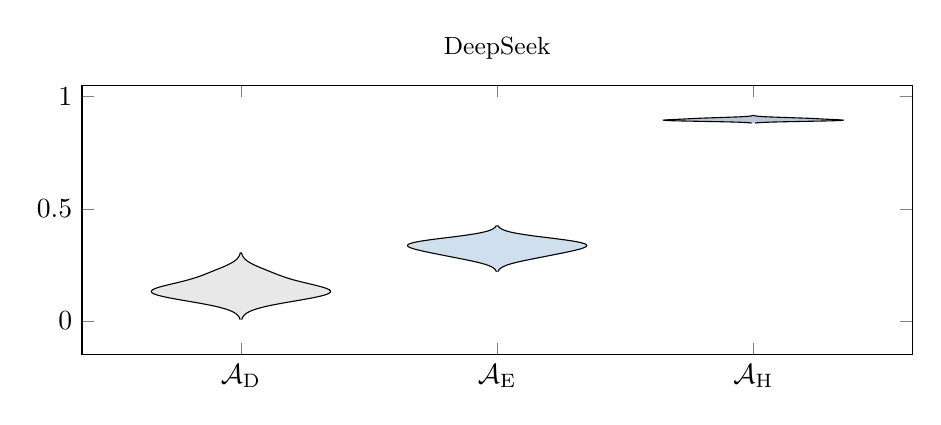
\begin{tikzpicture}
\begin{axis}[width=\textwidth, height=5cm, ymin=-0.15, ymax=1.05,
  xtick={1,2,3}, xticklabels={$\mathcal{A}_{\text{D}}$,$\mathcal{A}_{\text{E}}$,$\mathcal{A}_{\text{H}}$},
  title={\small DeepSeek}, title style={font=\small}]
\addplot[no marks, fill=colorPure!60, fill opacity=0.5] coordinates { (1.0030,0.0058) (1.0049,0.0119) (1.0076,0.0180) (1.0115,0.0240) (1.0170,0.0301) (1.0245,0.0362) (1.0344,0.0422) (1.0471,0.0483) (1.0629,0.0543) (1.0821,0.0604) (1.1046,0.0665) (1.1303,0.0725) (1.1586,0.0786) (1.1888,0.0846) (1.2199,0.0907) (1.2505,0.0968) (1.2792,0.1028) (1.3047,0.1089) (1.3254,0.1150) (1.3403,0.1210) (1.3486,0.1271) (1.3500,0.1331) (1.3447,0.1392) (1.3333,0.1453) (1.3170,0.1513) (1.2971,0.1574) (1.2753,0.1634) (1.2528,0.1695) (1.2309,0.1756) (1.2104,0.1816) (1.1917,0.1877) (1.1748,0.1937) (1.1595,0.1998) (1.1453,0.2059) (1.1318,0.2119) (1.1186,0.2180) (1.1054,0.2241) (1.0922,0.2301) (1.0791,0.2362) (1.0665,0.2422) (1.0545,0.2483) (1.0436,0.2544) (1.0340,0.2604) (1.0258,0.2665) (1.0190,0.2725) (1.0136,0.2786) (1.0095,0.2847) (1.0064,0.2907) (1.0042,0.2968) (1.0027,0.3029) (0.9973,0.3029) (0.9958,0.2968) (0.9936,0.2907) (0.9905,0.2847) (0.9864,0.2786) (0.9810,0.2725) (0.9742,0.2665) (0.9660,0.2604) (0.9564,0.2544) (0.9455,0.2483) (0.9335,0.2422) (0.9209,0.2362) (0.9078,0.2301) (0.8946,0.2241) (0.8814,0.2180) (0.8682,0.2119) (0.8547,0.2059) (0.8405,0.1998) (0.8252,0.1937) (0.8083,0.1877) (0.7896,0.1816) (0.7691,0.1756) (0.7472,0.1695) (0.7247,0.1634) (0.7029,0.1574) (0.6830,0.1513) (0.6667,0.1453) (0.6553,0.1392) (0.6500,0.1331) (0.6514,0.1271) (0.6597,0.1210) (0.6746,0.1150) (0.6953,0.1089) (0.7208,0.1028) (0.7495,0.0968) (0.7801,0.0907) (0.8112,0.0846) (0.8414,0.0786) (0.8697,0.0725) (0.8954,0.0665) (0.9179,0.0604) (0.9371,0.0543) (0.9529,0.0483) (0.9656,0.0422) (0.9755,0.0362) (0.9830,0.0301) (0.9885,0.0240) (0.9924,0.0180) (0.9951,0.0119) (0.9970,0.0058) };
\addplot[no marks, fill=colorRAG!60, fill opacity=0.5] coordinates { (2.0029,0.2192) (2.0045,0.2234) (2.0069,0.2275) (2.0101,0.2317) (2.0145,0.2359) (2.0203,0.2401) (2.0276,0.2442) (2.0367,0.2484) (2.0476,0.2526) (2.0602,0.2567) (2.0745,0.2609) (2.0902,0.2651) (2.1071,0.2693) (2.1248,0.2734) (2.1431,0.2776) (2.1616,0.2818) (2.1802,0.2859) (2.1988,0.2901) (2.2173,0.2943) (2.2357,0.2985) (2.2538,0.3026) (2.2715,0.3068) (2.2885,0.3110) (2.3045,0.3151) (2.3191,0.3193) (2.3315,0.3235) (2.3412,0.3277) (2.3476,0.3318) (2.3500,0.3360) (2.3479,0.3402) (2.3410,0.3443) (2.3291,0.3485) (2.3125,0.3527) (2.2914,0.3569) (2.2667,0.3610) (2.2393,0.3652) (2.2102,0.3694) (2.1806,0.3735) (2.1517,0.3777) (2.1245,0.3819) (2.0997,0.3861) (2.0779,0.3902) (2.0594,0.3944) (2.0441,0.3986) (2.0319,0.4027) (2.0225,0.4069) (2.0154,0.4111) (2.0103,0.4153) (2.0067,0.4194) (2.0042,0.4236) (1.9958,0.4236) (1.9933,0.4194) (1.9897,0.4153) (1.9846,0.4111) (1.9775,0.4069) (1.9681,0.4027) (1.9559,0.3986) (1.9406,0.3944) (1.9221,0.3902) (1.9003,0.3861) (1.8755,0.3819) (1.8483,0.3777) (1.8194,0.3735) (1.7898,0.3694) (1.7607,0.3652) (1.7333,0.3610) (1.7086,0.3569) (1.6875,0.3527) (1.6709,0.3485) (1.6590,0.3443) (1.6521,0.3402) (1.6500,0.3360) (1.6524,0.3318) (1.6588,0.3277) (1.6685,0.3235) (1.6809,0.3193) (1.6955,0.3151) (1.7115,0.3110) (1.7285,0.3068) (1.7462,0.3026) (1.7643,0.2985) (1.7827,0.2943) (1.8012,0.2901) (1.8198,0.2859) (1.8384,0.2818) (1.8569,0.2776) (1.8752,0.2734) (1.8929,0.2693) (1.9098,0.2651) (1.9255,0.2609) (1.9398,0.2567) (1.9524,0.2526) (1.9633,0.2484) (1.9724,0.2442) (1.9797,0.2401) (1.9855,0.2359) (1.9899,0.2317) (1.9931,0.2275) (1.9955,0.2234) (1.9971,0.2192) };
\addplot[no marks, fill=colorLLMParameterizedReferenceScoring!60, fill opacity=0.5] coordinates { (3.0070,0.8821) (3.0107,0.8828) (3.0161,0.8835) (3.0236,0.8841) (3.0336,0.8848) (3.0466,0.8855) (3.0631,0.8862) (3.0832,0.8869) (3.1070,0.8876) (3.1341,0.8883) (3.1640,0.8889) (3.1955,0.8896) (3.2275,0.8903) (3.2584,0.8910) (3.2866,0.8917) (3.3107,0.8924) (3.3296,0.8931) (3.3425,0.8938) (3.3492,0.8944) (3.3500,0.8951) (3.3457,0.8958) (3.3373,0.8965) (3.3262,0.8972) (3.3136,0.8979) (3.3005,0.8986) (3.2876,0.8992) (3.2754,0.8999) (3.2637,0.9006) (3.2524,0.9013) (3.2409,0.9020) (3.2288,0.9027) (3.2156,0.9034) (3.2010,0.9040) (3.1850,0.9047) (3.1677,0.9054) (3.1495,0.9061) (3.1308,0.9068) (3.1122,0.9075) (3.0943,0.9082) (3.0776,0.9089) (3.0625,0.9095) (3.0492,0.9102) (3.0378,0.9109) (3.0284,0.9116) (3.0209,0.9123) (3.0149,0.9130) (3.0105,0.9137) (3.0071,0.9143) (3.0048,0.9150) (3.0031,0.9157) (2.9969,0.9157) (2.9952,0.9150) (2.9929,0.9143) (2.9895,0.9137) (2.9851,0.9130) (2.9791,0.9123) (2.9716,0.9116) (2.9622,0.9109) (2.9508,0.9102) (2.9375,0.9095) (2.9224,0.9089) (2.9057,0.9082) (2.8878,0.9075) (2.8692,0.9068) (2.8505,0.9061) (2.8323,0.9054) (2.8150,0.9047) (2.7990,0.9040) (2.7844,0.9034) (2.7712,0.9027) (2.7591,0.9020) (2.7476,0.9013) (2.7363,0.9006) (2.7246,0.8999) (2.7124,0.8992) (2.6995,0.8986) (2.6864,0.8979) (2.6738,0.8972) (2.6627,0.8965) (2.6543,0.8958) (2.6500,0.8951) (2.6508,0.8944) (2.6575,0.8938) (2.6704,0.8931) (2.6893,0.8924) (2.7134,0.8917) (2.7416,0.8910) (2.7725,0.8903) (2.8045,0.8896) (2.8360,0.8889) (2.8659,0.8883) (2.8930,0.8876) (2.9168,0.8869) (2.9369,0.8862) (2.9534,0.8855) (2.9664,0.8848) (2.9764,0.8841) (2.9839,0.8835) (2.9893,0.8828) (2.9930,0.8821) };
\end{axis}
\end{tikzpicture}
\end{minipage}
\hfill
\begin{minipage}{0.24\textwidth}
\centering
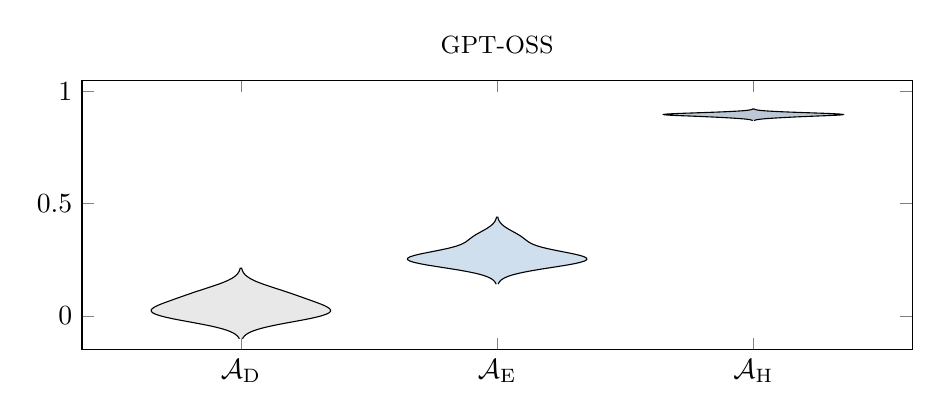
\begin{tikzpicture}
\begin{axis}[width=\textwidth, height=5cm, ymin=-0.15, ymax=1.05,
  xtick={1,2,3}, xticklabels={$\mathcal{A}_{\text{D}}$,$\mathcal{A}_{\text{E}}$,$\mathcal{A}_{\text{H}}$},
  title={\small GPT-OSS}, title style={font=\small}]
\addplot[no marks, fill=colorPure!60, fill opacity=0.5] coordinates { (1.0060,-0.1025) (1.0093,-0.0961) (1.0140,-0.0896) (1.0206,-0.0832) (1.0294,-0.0768) (1.0411,-0.0704) (1.0558,-0.0640) (1.0739,-0.0576) (1.0955,-0.0512) (1.1204,-0.0447) (1.1480,-0.0383) (1.1777,-0.0319) (1.2083,-0.0255) (1.2387,-0.0191) (1.2675,-0.0127) (1.2933,-0.0062) (1.3151,0.0002) (1.3320,0.0066) (1.3434,0.0130) (1.3494,0.0194) (1.3500,0.0258) (1.3459,0.0322) (1.3379,0.0387) (1.3269,0.0451) (1.3137,0.0515) (1.2991,0.0579) (1.2838,0.0643) (1.2681,0.0707) (1.2523,0.0772) (1.2365,0.0836) (1.2206,0.0900) (1.2046,0.0964) (1.1882,0.1028) (1.1714,0.1092) (1.1543,0.1156) (1.1370,0.1221) (1.1198,0.1285) (1.1029,0.1349) (1.0867,0.1413) (1.0716,0.1477) (1.0579,0.1541) (1.0458,0.1606) (1.0354,0.1670) (1.0267,0.1734) (1.0196,0.1798) (1.0141,0.1862) (1.0099,0.1926) (1.0067,0.1990) (1.0045,0.2055) (1.0029,0.2119) (0.9971,0.2119) (0.9955,0.2055) (0.9933,0.1990) (0.9901,0.1926) (0.9859,0.1862) (0.9804,0.1798) (0.9733,0.1734) (0.9646,0.1670) (0.9542,0.1606) (0.9421,0.1541) (0.9284,0.1477) (0.9133,0.1413) (0.8971,0.1349) (0.8802,0.1285) (0.8630,0.1221) (0.8457,0.1156) (0.8286,0.1092) (0.8118,0.1028) (0.7954,0.0964) (0.7794,0.0900) (0.7635,0.0836) (0.7477,0.0772) (0.7319,0.0707) (0.7162,0.0643) (0.7009,0.0579) (0.6863,0.0515) (0.6731,0.0451) (0.6621,0.0387) (0.6541,0.0322) (0.6500,0.0258) (0.6506,0.0194) (0.6566,0.0130) (0.6680,0.0066) (0.6849,0.0002) (0.7067,-0.0062) (0.7325,-0.0127) (0.7613,-0.0191) (0.7917,-0.0255) (0.8223,-0.0319) (0.8520,-0.0383) (0.8796,-0.0447) (0.9045,-0.0512) (0.9261,-0.0576) (0.9442,-0.0640) (0.9589,-0.0704) (0.9706,-0.0768) (0.9794,-0.0832) (0.9860,-0.0896) (0.9907,-0.0961) (0.9940,-0.1025) };
\addplot[no marks, fill=colorRAG!60, fill opacity=0.5] coordinates { (2.0040,0.1410) (2.0065,0.1471) (2.0102,0.1532) (2.0155,0.1593) (2.0230,0.1654) (2.0332,0.1715) (2.0467,0.1776) (2.0639,0.1837) (2.0852,0.1898) (2.1106,0.1959) (2.1398,0.2021) (2.1720,0.2082) (2.2061,0.2143) (2.2404,0.2204) (2.2732,0.2265) (2.3022,0.2326) (2.3258,0.2387) (2.3420,0.2448) (2.3500,0.2509) (2.3492,0.2570) (2.3400,0.2631) (2.3235,0.2692) (2.3013,0.2753) (2.2754,0.2814) (2.2479,0.2875) (2.2208,0.2937) (2.1958,0.2998) (2.1740,0.3059) (2.1559,0.3120) (2.1415,0.3181) (2.1303,0.3242) (2.1214,0.3303) (2.1141,0.3364) (2.1073,0.3425) (2.1004,0.3486) (2.0929,0.3547) (2.0845,0.3608) (2.0754,0.3669) (2.0658,0.3730) (2.0560,0.3791) (2.0464,0.3853) (2.0374,0.3914) (2.0294,0.3975) (2.0224,0.4036) (2.0167,0.4097) (2.0120,0.4158) (2.0084,0.4219) (2.0057,0.4280) (2.0038,0.4341) (2.0024,0.4402) (1.9976,0.4402) (1.9962,0.4341) (1.9943,0.4280) (1.9916,0.4219) (1.9880,0.4158) (1.9833,0.4097) (1.9776,0.4036) (1.9706,0.3975) (1.9626,0.3914) (1.9536,0.3853) (1.9440,0.3791) (1.9342,0.3730) (1.9246,0.3669) (1.9155,0.3608) (1.9071,0.3547) (1.8996,0.3486) (1.8927,0.3425) (1.8859,0.3364) (1.8786,0.3303) (1.8697,0.3242) (1.8585,0.3181) (1.8441,0.3120) (1.8260,0.3059) (1.8042,0.2998) (1.7792,0.2937) (1.7521,0.2875) (1.7246,0.2814) (1.6987,0.2753) (1.6765,0.2692) (1.6600,0.2631) (1.6508,0.2570) (1.6500,0.2509) (1.6580,0.2448) (1.6742,0.2387) (1.6978,0.2326) (1.7268,0.2265) (1.7596,0.2204) (1.7939,0.2143) (1.8280,0.2082) (1.8602,0.2021) (1.8894,0.1959) (1.9148,0.1898) (1.9361,0.1837) (1.9533,0.1776) (1.9668,0.1715) (1.9770,0.1654) (1.9845,0.1593) (1.9898,0.1532) (1.9935,0.1471) (1.9960,0.1410) };
\addplot[no marks, fill=colorLLMParameterizedReferenceScoring!60, fill opacity=0.5] coordinates { (3.0027,0.8703) (3.0043,0.8713) (3.0066,0.8724) (3.0099,0.8734) (3.0143,0.8745) (3.0201,0.8755) (3.0274,0.8766) (3.0363,0.8777) (3.0469,0.8787) (3.0591,0.8798) (3.0726,0.8808) (3.0873,0.8819) (3.1030,0.8829) (3.1195,0.8840) (3.1369,0.8850) (3.1552,0.8861) (3.1746,0.8871) (3.1953,0.8882) (3.2172,0.8892) (3.2403,0.8903) (3.2638,0.8914) (3.2869,0.8924) (3.3083,0.8935) (3.3266,0.8945) (3.3404,0.8956) (3.3484,0.8966) (3.3500,0.8977) (3.3450,0.8987) (3.3337,0.8998) (3.3170,0.9008) (3.2960,0.9019) (3.2720,0.9030) (3.2462,0.9040) (3.2197,0.9051) (3.1934,0.9061) (3.1679,0.9072) (3.1437,0.9082) (3.1212,0.9093) (3.1005,0.9103) (3.0818,0.9114) (3.0653,0.9124) (3.0509,0.9135) (3.0389,0.9145) (3.0289,0.9156) (3.0210,0.9167) (3.0148,0.9177) (3.0102,0.9188) (3.0068,0.9198) (3.0044,0.9209) (3.0028,0.9219) (2.9972,0.9219) (2.9956,0.9209) (2.9932,0.9198) (2.9898,0.9188) (2.9852,0.9177) (2.9790,0.9167) (2.9711,0.9156) (2.9611,0.9145) (2.9491,0.9135) (2.9347,0.9124) (2.9182,0.9114) (2.8995,0.9103) (2.8788,0.9093) (2.8563,0.9082) (2.8321,0.9072) (2.8066,0.9061) (2.7803,0.9051) (2.7538,0.9040) (2.7280,0.9030) (2.7040,0.9019) (2.6830,0.9008) (2.6663,0.8998) (2.6550,0.8987) (2.6500,0.8977) (2.6516,0.8966) (2.6596,0.8956) (2.6734,0.8945) (2.6917,0.8935) (2.7131,0.8924) (2.7362,0.8914) (2.7597,0.8903) (2.7828,0.8892) (2.8047,0.8882) (2.8254,0.8871) (2.8448,0.8861) (2.8631,0.8850) (2.8805,0.8840) (2.8970,0.8829) (2.9127,0.8819) (2.9274,0.8808) (2.9409,0.8798) (2.9531,0.8787) (2.9637,0.8777) (2.9726,0.8766) (2.9799,0.8755) (2.9857,0.8745) (2.9901,0.8734) (2.9934,0.8724) (2.9957,0.8713) (2.9973,0.8703) };
\end{axis}
\end{tikzpicture}
\end{minipage}
\hfill
\begin{minipage}{0.24\textwidth}
\centering
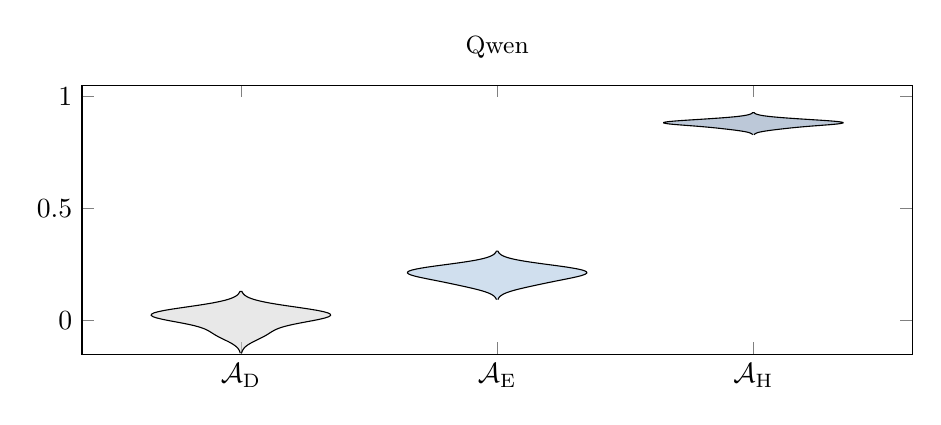
\begin{tikzpicture}
\begin{axis}[width=\textwidth, height=5cm, ymin=-0.15, ymax=1.05,
  xtick={1,2,3}, xticklabels={$\mathcal{A}_{\text{D}}$,$\mathcal{A}_{\text{E}}$,$\mathcal{A}_{\text{H}}$},
  title={\small Qwen}, title style={font=\small}]
\addplot[no marks, fill=colorPure!60, fill opacity=0.5] coordinates { (1.0025,-0.1452) (1.0039,-0.1396) (1.0058,-0.1340) (1.0086,-0.1283) (1.0122,-0.1227) (1.0169,-0.1171) (1.0228,-0.1115) (1.0299,-0.1059) (1.0382,-0.1003) (1.0473,-0.0946) (1.0572,-0.0890) (1.0673,-0.0834) (1.0774,-0.0778) (1.0871,-0.0722) (1.0960,-0.0666) (1.1043,-0.0610) (1.1121,-0.0553) (1.1199,-0.0497) (1.1283,-0.0441) (1.1382,-0.0385) (1.1505,-0.0329) (1.1658,-0.0273) (1.1845,-0.0216) (1.2065,-0.0160) (1.2312,-0.0104) (1.2574,-0.0048) (1.2837,0.0008) (1.3079,0.0064) (1.3283,0.0121) (1.3428,0.0177) (1.3500,0.0233) (1.3490,0.0289) (1.3397,0.0345) (1.3224,0.0401) (1.2983,0.0458) (1.2691,0.0514) (1.2365,0.0570) (1.2025,0.0626) (1.1689,0.0682) (1.1373,0.0738) (1.1087,0.0794) (1.0838,0.0851) (1.0629,0.0907) (1.0460,0.0963) (1.0328,0.1019) (1.0227,0.1075) (1.0153,0.1131) (1.0101,0.1188) (1.0065,0.1244) (1.0040,0.1300) (0.9960,0.1300) (0.9935,0.1244) (0.9899,0.1188) (0.9847,0.1131) (0.9773,0.1075) (0.9672,0.1019) (0.9540,0.0963) (0.9371,0.0907) (0.9162,0.0851) (0.8913,0.0794) (0.8627,0.0738) (0.8311,0.0682) (0.7975,0.0626) (0.7635,0.0570) (0.7309,0.0514) (0.7017,0.0458) (0.6776,0.0401) (0.6603,0.0345) (0.6510,0.0289) (0.6500,0.0233) (0.6572,0.0177) (0.6717,0.0121) (0.6921,0.0064) (0.7163,0.0008) (0.7426,-0.0048) (0.7688,-0.0104) (0.7935,-0.0160) (0.8155,-0.0216) (0.8342,-0.0273) (0.8495,-0.0329) (0.8618,-0.0385) (0.8717,-0.0441) (0.8801,-0.0497) (0.8879,-0.0553) (0.8957,-0.0610) (0.9040,-0.0666) (0.9129,-0.0722) (0.9226,-0.0778) (0.9327,-0.0834) (0.9428,-0.0890) (0.9527,-0.0946) (0.9618,-0.1003) (0.9701,-0.1059) (0.9772,-0.1115) (0.9831,-0.1171) (0.9878,-0.1227) (0.9914,-0.1283) (0.9942,-0.1340) (0.9961,-0.1396) (0.9975,-0.1452) };
\addplot[no marks, fill=colorRAG!60, fill opacity=0.5] coordinates { (2.0028,0.0937) (2.0045,0.0981) (2.0068,0.1026) (2.0101,0.1070) (2.0145,0.1114) (2.0203,0.1158) (2.0277,0.1202) (2.0368,0.1246) (2.0476,0.1290) (2.0602,0.1334) (2.0742,0.1378) (2.0895,0.1422) (2.1059,0.1466) (2.1229,0.1510) (2.1405,0.1554) (2.1584,0.1598) (2.1766,0.1642) (2.1952,0.1687) (2.2141,0.1731) (2.2333,0.1775) (2.2528,0.1819) (2.2722,0.1863) (2.2910,0.1907) (2.3087,0.1951) (2.3242,0.1995) (2.3369,0.2039) (2.3457,0.2083) (2.3500,0.2127) (2.3492,0.2171) (2.3430,0.2215) (2.3315,0.2259) (2.3149,0.2303) (2.2939,0.2347) (2.2694,0.2392) (2.2422,0.2436) (2.2135,0.2480) (2.1844,0.2524) (2.1560,0.2568) (2.1291,0.2612) (2.1045,0.2656) (2.0826,0.2700) (2.0638,0.2744) (2.0481,0.2788) (2.0354,0.2832) (2.0254,0.2876) (2.0177,0.2920) (2.0121,0.2964) (2.0080,0.3008) (2.0052,0.3053) (2.0032,0.3097) (1.9968,0.3097) (1.9948,0.3053) (1.9920,0.3008) (1.9879,0.2964) (1.9823,0.2920) (1.9746,0.2876) (1.9646,0.2832) (1.9519,0.2788) (1.9362,0.2744) (1.9174,0.2700) (1.8955,0.2656) (1.8709,0.2612) (1.8440,0.2568) (1.8156,0.2524) (1.7865,0.2480) (1.7578,0.2436) (1.7306,0.2392) (1.7061,0.2347) (1.6851,0.2303) (1.6685,0.2259) (1.6570,0.2215) (1.6508,0.2171) (1.6500,0.2127) (1.6543,0.2083) (1.6631,0.2039) (1.6758,0.1995) (1.6913,0.1951) (1.7090,0.1907) (1.7278,0.1863) (1.7472,0.1819) (1.7667,0.1775) (1.7859,0.1731) (1.8048,0.1687) (1.8234,0.1642) (1.8416,0.1598) (1.8595,0.1554) (1.8771,0.1510) (1.8941,0.1466) (1.9105,0.1422) (1.9258,0.1378) (1.9398,0.1334) (1.9524,0.1290) (1.9632,0.1246) (1.9723,0.1202) (1.9797,0.1158) (1.9855,0.1114) (1.9899,0.1070) (1.9932,0.1026) (1.9955,0.0981) (1.9972,0.0937) };
\addplot[no marks, fill=colorLLMParameterizedReferenceScoring!60, fill opacity=0.5] coordinates { (3.0027,0.8291) (3.0043,0.8311) (3.0066,0.8331) (3.0098,0.8352) (3.0142,0.8372) (3.0199,0.8392) (3.0270,0.8412) (3.0358,0.8432) (3.0461,0.8452) (3.0579,0.8472) (3.0709,0.8492) (3.0850,0.8512) (3.0998,0.8532) (3.1152,0.8552) (3.1311,0.8573) (3.1477,0.8593) (3.1652,0.8613) (3.1839,0.8633) (3.2039,0.8653) (3.2254,0.8673) (3.2480,0.8693) (3.2710,0.8713) (3.2935,0.8733) (3.3139,0.8753) (3.3310,0.8773) (3.3434,0.8794) (3.3499,0.8814) (3.3500,0.8834) (3.3435,0.8854) (3.3308,0.8874) (3.3128,0.8894) (3.2905,0.8914) (3.2652,0.8934) (3.2380,0.8954) (3.2102,0.8974) (3.1826,0.8994) (3.1559,0.9015) (3.1309,0.9035) (3.1079,0.9055) (3.0873,0.9075) (3.0691,0.9095) (3.0536,0.9115) (3.0406,0.9135) (3.0300,0.9155) (3.0217,0.9175) (3.0152,0.9195) (3.0104,0.9215) (3.0069,0.9236) (3.0045,0.9256) (3.0028,0.9276) (2.9972,0.9276) (2.9955,0.9256) (2.9931,0.9236) (2.9896,0.9215) (2.9848,0.9195) (2.9783,0.9175) (2.9700,0.9155) (2.9594,0.9135) (2.9464,0.9115) (2.9309,0.9095) (2.9127,0.9075) (2.8921,0.9055) (2.8691,0.9035) (2.8441,0.9015) (2.8174,0.8994) (2.7898,0.8974) (2.7620,0.8954) (2.7348,0.8934) (2.7095,0.8914) (2.6872,0.8894) (2.6692,0.8874) (2.6565,0.8854) (2.6500,0.8834) (2.6501,0.8814) (2.6566,0.8794) (2.6690,0.8773) (2.6861,0.8753) (2.7065,0.8733) (2.7290,0.8713) (2.7520,0.8693) (2.7746,0.8673) (2.7961,0.8653) (2.8161,0.8633) (2.8348,0.8613) (2.8523,0.8593) (2.8689,0.8573) (2.8848,0.8552) (2.9002,0.8532) (2.9150,0.8512) (2.9291,0.8492) (2.9421,0.8472) (2.9539,0.8452) (2.9642,0.8432) (2.9730,0.8412) (2.9801,0.8392) (2.9858,0.8372) (2.9902,0.8352) (2.9934,0.8331) (2.9957,0.8311) (2.9973,0.8291) };
\end{axis}
\end{tikzpicture}
\end{minipage}
\caption{Violin plots of Kendall's $\tau$ across five runs.}
\end{threeparttable}
\label{fig:violin_tau}
\end{figure*}

The results above are five-run averages for Kendall's $\tau$. To assess trial-to-trial stability, we computed every metric independently for each of the five runs per architecture per model. Figure~\ref{fig:violin_tau} (violin plot) shows the $\tau$ distributions, and Figure~\ref{fig:violin_rmse} (strip plot, Appendix~\ref{app:variance}) shows the RMSE distributions.
\FloatBarrier

RMSE, which penalizes large errors more than MAE, shows the same architecture separation. $\mathcal{A}_{\text{H}}$ RMSE is $< 0.11$ for three of four models across every run, while $\mathcal{A}_{\text{D}}$'s RMSE is always more than 0.29. The Qwen $\mathcal{A}_{\text{H}}$ box shows a wider interquartile range (RMSE $\in [0.157, 0.167]$), reflecting the GPM estimation imprecision that also limits its $\tau$. The full RMSE distribution appears in Appendix~\ref{app:variance}; mean $\pm$ std for MAE and Top-1 accuracy across runs appears in Table~\ref{tab:overall_by_model} (Appendix~\ref{app:numerical_results}).


\FloatBarrier
\section{Discussion}
\label{sec:discussion}

\subsection{Interpretation of Results}
\label{sec:interpretation}

$\mathcal{A}_{\text{H}}$ compresses model capability into a narrow performance band: its $\tau$ spans only 0.043 across a 45$\times$ range of per-run model cost (Gemini 0.923 to Qwen 0.880), compared to 0.166 for $\mathcal{A}_{\text{D}}$ and 0.121 for $\mathcal{A}_{\text{E}}$. GPT-OSS-20B illustrates the point: despite a 12.0\% extraction failure rate on $\mathcal{A}_{\text{H}}$ (all recovered by cross-run averaging), its $\tau$ of 0.897 lands closer to Gemini's 0.923 than to its own $\mathcal{A}_{\text{D}}$ score of 0.041.

The ranking advantage of $\mathcal{A}_{\text{H}}$ is partly structural (see Section~\ref{sec:architectures}). MAE results confirm extraction accuracy (see Section~\ref{sec:res-error}). For energy cost, this MAE corresponds to roughly \$0.20 per scenario; for environmental impact, approximately 1.4 lbs CO$_2$ (HVAC/Appliance) or 3 gallons of water (Shower), using the reference ranges in Table~\ref{table:reference_ranges}. Model choice drives most score-level error (ICC(2,1) = 0.80--0.83 for MAE), but under the prompts and models tested, architecture explains more performance variation than model choice.

This robustness is not a property of extraction accuracy improving; it is a property of decision structure. Because the LLM estimates scenario-level parameters that enter every alternative identically, an error shifts the whole choice set rather than any single alternative and largely cancels when the calculator ranks. That cancellation should hold wherever the alternatives share an underlying, jointly-uncertain state, as they do throughout this benchmark's within-household choice sets, but it weakens for a parameter that both scales the outcome directly and is recovered from a coarse homeowner-facing proxy, as Shower GPM demonstrates (Section~\ref{sec:res-extraction}). The parameter-provenance ablation (Section~\ref{sec:res-paramprov}) locates where the resulting accuracy actually comes from: calculator access alone, with no per-scenario inference, reaches only $\tau = 0.641$, so roughly a quarter of $\mathcal{A}_{\text{H}}$'s advantage is attributable to the LLM's extraction rather than to the calculator doing the work unaided. Deploying $\mathcal{A}_{\text{H}}$ on decisions where alternatives do not share a common underlying parameter set, comparing unrelated households or services rather than variants of the same scenario, would remove this cancellation effect and remains untested here.

The RAG ablation study (Figure~\ref{fig:rag_ablation}) confirms that exemplar scores anchor the LLM's output scale, counteracting the central-tendency bias that otherwise collapses scores toward 0.5. Removing scores drops $\tau$ from 0.277 to 0.068, while removing hidden engineering parameters has negligible effect ($\tau = 0.279$ versus 0.277): the LLM infers engineering parameters from scenario context, making them redundant. Semantic selection of exemplars drives the RAG contribution (random exemplars yield $\tau = 0.121$), while retrieval architecture and exemplar content contribute negligibly (top-cluster pairwise $p_{\text{Holm}} > 0.62$). The practical implication is that investing in pre-scored exemplars matters more than enriching exemplar content.

$\mathcal{A}_{\text{D}}$'s central-tendency bias (Section~\ref{sec:mavt-design}) is most damaging under high task dimensionality (Section~\ref{sec:res-bytype}).

$\mathcal{A}_{\text{E}}$ achieves 80\% Top-2 across models: the ground-truth best alternative appears in the architecture's top two four times out of five. Top-2's practical sufficiency depends on the decision domain: when the cost gap between first and second place is large, Top-1 accuracy matters, but when the alternatives are closely matched, Top-2 provides actionable guidance. $\mathcal{A}_{\text{H}}$ at 97.8\% Top-2 avoids this issue: the best alternative is almost always in the recommended pair.

An entropy-based weight analysis, reported in Appendix~\ref{app:weights}, supports the assumed 35/30/20/15 weighting scheme: entropy and MEREC methods assign above-average weight to the Environmental criterion, consistent with the a priori design, while implied weights collapse toward criteria with the most within-scenario variance---a methodological finding rather than an indictment of the design weights.

$\mathcal{A}_{\text{H}}$ was the strongest architecture overall. This central-tendency avoidance corroborates Li et al. (2026) and Zhu et al. (2026), who documented systematic scoring biases in LLM-as-judge pipelines; $\mathcal{A}_{\text{H}}$ sidesteps these biases by removing the LLM from the scoring role entirely. The MAE reduction relative to $\mathcal{A}_{\text{E}}$ is large in absolute terms; delegating arithmetic to a vetted reference model proves more reliable than asking the LLM to score directly. $\mathcal{A}_{\text{H}}$'s primary limitation is reliance on the calculator: if the calculator cannot model a criterion (e.g., user practicality), the architecture falls back on the same weaknesses as other architectures.

Each architecture trades upfront setup effort against output accuracy and runtime cost. Direct scoring ($\mathcal{A}_{\text{D}}$) needs no custom code, but scores cluster near 0.5 ($\tau = 0.093$). Example-guided scoring ($\mathcal{A}_{\text{E}}$) requires building a database of past cases and sending larger prompts, reaching $\tau = 0.277$. Parameterized scoring ($\mathcal{A}_{\text{H}}$) requires writing domain equations first, but reduces API prompts to one call per scenario while reaching $\tau = 0.899$. $\mathcal{A}_{\text{H}}$ is also the most cost-efficient architecture: one API call per scenario at roughly 600 tokens versus three calls at 2,000--3,400 tokens (Table~\ref{tab:item8}), yielding per-run costs of \$0.006--\$0.280 versus \$0.023--\$1.024 for $\mathcal{A}_{\text{E}}$.

The $\mathcal{A}_{\text{H}}$ design generalizes to any domain with a verifiable ground-truth function (Section~\ref{sec:futurework}). The LLM estimates input parameters and the calculator produces scores, sidestepping uncalibrated LLM scoring. The dimensionality analysis in Section~\ref{sec:res-bytype} suggests a deployment heuristic: $\mathcal{A}_{\text{H}}$'s accuracy advantage is largest for high-dimensional decisions ($\geq$4 interacting parameters) and narrows for low-dimensional decisions ($\leq$3 parameters).

\subsection{Comparison with Prior Work}
\label{sec:comparison}

Svoboda and Lande (2024) showed that GPT-4 can construct an AHP model with a consistency ratio below the 0.10 threshold \cite{svoboda2024}; Shekhovtsov et al.\ (2026) reported that structured output formats improve ranking consistency in COMET-based MCDA \cite{icaart26}. Our $\mathcal{A}_{\text{D}}$ results qualify both findings: the model generates well-formed JSON and constrained schemas with near-zero $\tau$ variance across runs, yet the rankings themselves are wrong. Internal consistency and ground-truth accuracy diverge because the central-tendency bias compresses scores into a narrow middle band, missing the sharp non-linear penalties in the value functions. Structured output is necessary but not sufficient; the type of task matters. Scoring demands numeracy that extraction does not. This central-tendency pattern generalizes the scoring biases documented by Wang et al.\ (2024), Li et al.\ (2026), Zhu et al.\ (2026), and Poličar et al.\ (2025) from judge contexts to multi-criteria decision scoring, where the consequences reach beyond fairness concerns into incorrect decisions with real resource-allocation impacts. To our knowledge, this is the first study to benchmark this failure mode against a deterministic reference calculator.

The $\mathcal{A}_{\text{E}}$ architecture follows Case-Based Reasoning (Aamodt and Plaza, 1994) \cite{aamodtplaza1994}: retrieved exemplars anchor the LLM's scoring output. Wiratunga et al.\ (2024) and Minor and Kaucher (2024) demonstrated this effect in legal and business-process domains \cite{wiratunga2024cbrrag,minorkaucher2024}. Our results replicate the finding in MCDA, with $\tau$ improving by 0.19--0.28 over $\mathcal{A}_{\text{D}}$. The gain plateaus, however, because exemplar scores function as calibration anchors that set the output scale but cannot compensate for the underlying central-tendency bias. The RAG ablation in Section~\ref{sec:rag-ablation} confirms this mechanism: removing exemplars degrades performance roughly as much as removing the scoring prompt itself, suggesting the LLM treats both as scale-setting signals rather than learning the value function shape. This explains why the improvement caps out relative to the legal and business domains where CBR was first demonstrated.

Rather than improving the LLM's arithmetic capability through chain-of-thought prompting or tool augmentation \cite{schick2023toolformer,gao2023pal}, $\mathcal{A}_{\text{H}}$ bypasses the numeracy problem entirely \cite{cobbe2021gsm8k,imani2023mathprompter}. The architecture requires only a single structured extraction call and a function call to an existing calculator: no fine-tuning, no few-shot engineering, no prompt-embedded arithmetic. This simplicity is itself a contribution. Fewer failure modes, lower cost, easier verification. Huang and Burgherr (2024) built a streamlined MCDA calculator that still requires users to possess MCDA expertise; $\mathcal{A}_{\text{H}}$ eliminates that barrier by having the LLM bridge natural-language context to domain-specific parameters.

\subsection{Limitations of the Study}
\label{sec:limitations}

The limitations fall into three groups: threats to the magnitude of $\mathcal{A}_{\text{H}}$'s advantage, threats to external validity, and scope boundaries.

\subsubsection{Threats to the Magnitude of $\mathcal{A}_{\text{H}}$'s Advantage}

Prompt design is a potential confound in the architecture comparison. The prompt-sensitivity ablation (Section~\ref{sec:prompt-ablation}) addresses this directly for $\mathcal{A}_{\text{D}}$ and $\mathcal{A}_{\text{E}}$: across three controlled perturbations, three models, and five runs each, the architecture ordering survived every variant, and the shipped prompts were not an unlucky draw. This narrows, rather than eliminates, the concern. The ablation excluded Gemini for cost reasons, and it never perturbed $\mathcal{A}_{\text{H}}$'s extraction prompt, so whether the $\mathcal{A}_{\text{H}}$ advantage over $\mathcal{A}_{\text{D}}$ and $\mathcal{A}_{\text{E}}$ specifically reflects a fortunate extraction-prompt draw rather than the architecture itself remains open. The RAG ablation (Section~\ref{sec:interpretation}) offers separate partial evidence bearing on $\mathcal{A}_{\text{E}}$'s exemplar-related prompt structure, but that result speaks to the exemplar mechanism, not to $\mathcal{A}_{\text{H}}$'s extraction prompt. Extending the prompt-variant robustness check to $\mathcal{A}_{\text{H}}$ and to Gemini (Section~\ref{sec:futurework}) would close this gap.

The same researcher designed both the $\mathcal{A}_{\text{H}}$ parameter-extraction schema and the ground-truth calculators' input schemas, raising a potential circular-validation risk. The key distinction is that $\mathcal{A}_{\text{H}}$ does not receive a separate or easier scoring function: it uses the same deterministic calculator as the ground truth, but with several calculator inputs withheld and estimated from homeowner-accessible scenario text. The ground truth represents a fully specified calculation with exact engineering parameters; $\mathcal{A}_{\text{H}}$ represents the deployable case where those parameters must be inferred before the same calculator can run. This design still benefits from a shared author, but the comparison is not circular in the sense of giving $\mathcal{A}_{\text{H}}$ direct access to ground-truth scores or hidden calculator mappings. A sharper concern is whether the physical validation bounds (R-value, SEER, GPM ranges) were chosen to be lenient enough for LLM estimates. The bounds derive from ASHRAE and ENERGY STAR literature spanning the full residential range, not from pilot LLM outputs. Nonetheless, a blind schema review by an independent engineer would strengthen this claim.

\subsubsection{Calculator Simplifications}
\label{sec:calculator-simplifications}

Five engineering imputations in the ground-truth calculators introduce systematic error: linear interpolation of mains water temperature from outdoor temperature, fixed monthly appliance cycle rates in place of observed utilization, a fixed 0.8 shower tank-availability factor, discrete banding of insulation and appliance age, and a run-time-fraction approximation of HVAC occupancy (full derivations in Appendix~\ref{app:utility_derivations}). Each affects all architectures equally and does not bias the architecture comparison. The absolute MAE and RMSE values reflect the combined error of LLM extraction and calculator imputation; a perfect LLM extractor would produce non-zero MAE if the ground truth deviates from measured household data.

Beyond parametric simplifications, the calculator's functional form could be misspecified. If the HVAC load decomposition (Eq.~\ref{eq:hvac_cooling_load}) or the shower mixing model (Eq.~\ref{eq:shower_fraction}) is structurally wrong, $\mathcal{A}_{\text{H}}$ inherits that error perfectly while $\mathcal{A}_{\text{D}}$ and $\mathcal{A}_{\text{E}}$, being independent of the calculator, could in principle produce correct rankings where the calculator fails. The five imputations above affect all architectures equally, but a structural misspecification would penalize $\mathcal{A}_{\text{H}}$ alone---a qualitatively different failure mode that the current benchmark cannot detect.

Results are specific to Pennsylvania's grid and utility rate structure. The PJM marginal emissions factors (peak: 1.041~lbs~CO$_2$/kWh; off-peak: 0.976~lbs~CO$_2$/kWh) and Pennsylvania time-of-use rate tiers do not generalize to high-renewables grids, where lower and more variable emissions intensities would compress environmental score distributions. The architecture ordering is large enough that it would likely persist, but the absolute MAE values for environmental and energy-cost criteria would shift.

The environmental criterion for shower decisions uses water consumption in gallons rather than CO$_2$ emissions. HVAC and Appliance environmental scores reflect grid emissions; Shower environmental scores reflect water volume. Cross-type comparisons of environmental MAE should account for this distinction; within-type ranking validity is unaffected. All shower scenarios assume electric resistance water heating; gas, heat-pump, and tankless configurations are outside the current scope.

\subsubsection{Threats to External Validity}

The scenario corpus was generated by crossing categorical parameters with representative numeric draws. This combinatorial distribution ensures parameter-space coverage but does not reflect real-world joint distributions---in practice, older houses tend to have worse insulation and lower SEER ratings together. The synthetic corpus decouples these correlations, potentially making ranking easier or harder than in household populations. This affects all architectures equally and does not bias the comparison, but it bounds external validity.

Temperature 0.3 and the five-run-then-average protocol were methodological choices. Lower temperatures reduce variance but may increase central-tendency bias; higher temperatures increase diversity but risk incoherent outputs. The reported absolute metric values are specific to this operating point, though the architecture ordering appears robust.

A further limitation concerns the choice sets supplied to the architectures. In this benchmark, each scenario presents three specific alternatives that a household might compare. In practice, households rarely know three specific alternatives they want to evaluate; the decision space is continuous and often unstructured. With $n=3$ alternatives, there are only $3! = 6$ possible rankings, and $\mathcal{A}_{\text{H}}$'s scenario-level parameter estimation produces correlated errors across alternatives that are more likely to cancel in a 3-alternative ranking than in larger choice sets. The ``smoothness'' claim---that three bands around the same times as the specific alternatives programmed in our test scenarios would produce similar overall results---rests on the assumption that the value functions are monotonic over the relevant ranges, which holds for cost and energy criteria but may not hold for comfort. The benchmark tests ranking accuracy, not choice generation; extending the framework to open-ended alternative generation would be a next step. The reported $\tau$ of 0.899 should be interpreted as an upper bound on $\mathcal{A}_{\text{H}}$'s ranking accuracy for larger choice sets.

\subsubsection{Scope Boundaries}

The framework assumes a single decision-maker with fixed weights. Real households contain multiple occupants with conflicting preferences---different thermostat setpoints, shower durations, appliance schedules. $\mathcal{A}_{\text{H}}$'s cheap single-call extraction makes multi-vector evaluation practical (one extraction, $N$ weight passes), but this was not tested. Eliciting and aggregating multi-occupant preferences \cite{keeneyraiffa1976} is left to future work.

A more fundamental constraint concerns the implementation cost of the
$\mathcal{A}_{\text{H}}$ architecture itself. The three ground-truth calculators developed
for this study, covering HVAC load estimation, appliance TOU scheduling,
and shower thermodynamics, each required extensive domain research,
iterative calibration, and verification against published standards
(ASHRAE, ENERGY STAR, EPA eGRID). In practice, this engineering effort
constituted the majority of the total project time. This cost does not
diminish $\mathcal{A}_{\text{H}}$'s accuracy advantage, but it bounds its practical
applicability: $\mathcal{A}_{\text{H}}$ is the appropriate architecture when a vetted,
domain-specific calculator already exists or is worth building for the
decision at hand. For decision domains where no such calculator exists
and the cost of developing one is prohibitive, $\mathcal{A}_{\text{E}}$ or
sufficiently capable $\mathcal{A}_{\text{D}}$ may remain the only accessible
options, even at a known accuracy cost. This tradeoff is the primary
practical implication of RQ2 and should be weighed before
adopting the $\mathcal{A}_{\text{H}}$ approach in new domains.



\subsection{Future Work}
\label{sec:futurework}
Future work falls into three tiers ordered by cost and proximity to the current results.

The most immediate follow-ups directly strengthen this paper's claims: extending the prompt-sensitivity ablation (Section~\ref{sec:prompt-ablation}) to $\mathcal{A}_{\text{H}}$'s extraction prompt and to Gemini, and an independent schema review, an engineer who did not build the calculators auditing $\mathcal{A}_{\text{H}}$'s extraction schema and validation bounds, to address the single-researcher circularity concern raised in Section~\ref{sec:limitations}.

A second tier would test generalization: cross-grid replication under different emissions--cost correlation structures (e.g., ERCOT's real-time pricing or a high-nuclear European grid where marginal emissions approach zero during surplus, addressing the PJM specificity noted in Section~\ref{sec:limitations}), a domain-transfer test applying $\mathcal{A}_{\text{H}}$ to a mature calculator outside energy (e.g., actuarial life-expectancy or portfolio Sharpe-ratio estimation), and an adversarial stress test that deliberately violates the calculators' structural assumptions to identify where $\mathcal{A}_{\text{H}}$'s advantage degrades.

A third, longer-term tier would extend the framework's scope: a neurosymbolic verification layer checking extracted outputs against known physical bounds \cite{mattas2026neurosymbolic,ye2023satlm}, multi-turn preference elicitation from multiple household members to move beyond the single-decision-maker assumption (Section~\ref{sec:limitations}), and a randomized controlled trial comparing LLM-MCDA recommendations against unaided decisions over a sustained household deployment.

\FloatBarrier
\section{Conclusion}
\label{sec:conclusion}
This study benchmarked three strategies for integrating an LLM into an MCDA workflow for household energy decisions (direct $\mathcal{A}_{\text{D}}$, $\mathcal{A}_{\text{E}}$ prompting, and $\mathcal{A}_{\text{H}}$, which uses the LLM only to extract withheld engineering parameters and a deterministic physics calculator to score) against a deterministic MAVT reference calculator across HVAC, Appliance, and Shower decisions. Throughout, accuracy means agreement with the reference calculator, not measured household energy data. $\mathcal{A}_{\text{H}}$ most accurately replicates the reference calculator and compresses the model-capability gap (RQ1), and this ordering held across all four models, though the gap between architectures narrowed for weaker models (RQ2). Section~\ref{sec:limitations} states the two principal threats that bound this generalization: one researcher designed both the calculator and the $\mathcal{A}_{\text{H}}$ extractor, and the single-grid (Pennsylvania/PJM) specificity of the ground truth.

For households, the decision tool works from a natural-language description without requiring MCDA expertise: describe the situation, receive a ranked recommendation backed by transparent physics. For grid planners and demand-response programs, the architecture scales to millions of household decisions, each scored consistently against the same engineering standards, without the per-scenario expert effort that traditional MCDA demands.

Build the deterministic calculator once, and cheaper models match the ranking accuracy of expensive ones, making production deployment economically viable. Whether the architecture generalizes across grids, domains, and household populations (Section~\ref{sec:futurework}) is the question the next study should answer.

\clearpage

\paragraph*{Declaration of competing interest}
The authors declare that they have no known competing financial interests or personal relationships that could have appeared to influence the work reported in this paper.

\paragraph*{Funding}
This research did not receive any specific grant from funding agencies in the public, commercial, or not-for-profit sectors.

\paragraph*{CRediT authorship contribution statement}
\textbf{Ahaan Nigam:} Conceptualization, Methodology, Software, Validation, Formal analysis, Investigation, Data Curation, Writing --- Original Draft, Writing --- Review \& Editing, Visualization. \textbf{River Huang:} Validation, Conceptualization, Methodology, Supervision, Writing --- Review \& Editing.

\paragraph*{Software and data availability}
Name of software/dataset: LLM-MCDA-Paper (benchmark code, ground-truth calculators, and scenario/RAG data). Developer and contact: Ahaan Nigam (\href{mailto:ishaannigam27@gmail.com}{ishaannigam27@gmail.com}). Year first available: 2026. Hardware required: none beyond a standard desktop/laptop capable of running Python 3.11+; network access to the OpenRouter API for LLM calls. Software required: Python 3.11+ with the packages listed in the repository's dependency file (pandas, openpyxl, chromadb, sentence-transformers). Program language: Python. Availability and cost: free, openly available. Repository form: public Git repository containing source code, Excel-format ground-truth and scenario data, and raw run outputs. Access: \url{https://github.com/AN00927/LLM-MCDA-Paper}.

\paragraph*{Declaration of generative AI and AI-assisted technologies in the manuscript preparation process}
During the preparation of this work the author(s) used [TODO: NAME OF TOOL/SERVICE] in order to [TODO: REASON]. After using this tool/service, the author(s) reviewed and edited the content as needed and take(s) full responsibility for the content of the published article.

\bibliographystyle{elsarticle-num}
\bibliography{cas-refs}
\newpage

\appendix
\section{Notation}
\label{app:notation}
\begin{table}[t]
\begin{threeparttable}
\small
\centering
\renewcommand{\arraystretch}{1.15}
\begin{tabular}{ll}
\toprule
Symbol & Definition \\
\midrule
$\tau$ & Kendall's rank correlation coefficient \\
$w_i$ & weight of criterion $i$ ($i=1\ldots4$), summing to 1 \\
$v_i(x)$ & value function score for criterion $i$ at raw value $x$, range $[0,1]$ \\
$\alpha$ & shape parameter for logarithmic value functions \\
$s_j$ & MAVT weighted sum score for alternative $j$ \\
$\text{MAE}$ & Mean Absolute Error on MAVT score (0--1 scale) \\
$\text{RMSE}$ & Root Mean Squared Error on MAVT score (0--1 scale) \\
$n$ & number of test scenarios evaluated \\
$k$ & number of retrieved scenarios per query in RAG ($k=1$) \\
\bottomrule
\end{tabular}
\renewcommand{\arraystretch}{1.0}
\caption{Notation used throughout this paper.}
\label{tab:item1}
\end{threeparttable}
\end{table}

\section{Full Parameter Comparison Tables}
\label{app:parameter_comparison_full}

Table~\ref{tab:parameter_comparison_full} lists the Appliance and Shower parameter visibility, following the same LLM-visible/calculator-visible split shown for HVAC in Table~\ref{tab:parameter_comparison} (Section~\ref{sec2}).

\begin{table}[H]
\begin{threeparttable}
\centering
\footnotesize
\renewcommand{\arraystretch}{0.88}
\caption{Scenario parameters available to LLM architectures vs.\ ground-truth calculators (Appliance and Shower).}
\label{tab:parameter_comparison_full}
\begin{minipage}[t]{0.47\textwidth}\vspace{0pt}
\centering
\textbf{Appliance}\\[0.3em]
\begin{tabular}{@{} l c c @{}}
\toprule
\textbf{Parameter} & \textbf{LLMs} & \textbf{Calc.} \\
\midrule
Appliance Type          & T          & \checkmark \\
Baseline Runtime        & T          & \checkmark \\
Appliance Age Tier      & \checkmark & ---        \\
kWh per Cycle           & ---        & \checkmark \\
TOU Period / Utility Rate & ---      & \checkmark \\
Monthly Cycles          & ---        & \checkmark \\
Household Size          & \checkmark & \checkmark \\
Housing Type            & \checkmark & \checkmark \\
Location                & \checkmark & \checkmark \\
Utility Budget          & \checkmark & \checkmark \\
\bottomrule
\end{tabular}
\end{minipage}%
\hfill
\begin{minipage}[t]{0.47\textwidth}\vspace{0pt}
\centering
\textbf{Shower}\\[0.3em]
\begin{tabular}{@{} l c c @{}}
\toprule
\textbf{Parameter} & \textbf{LLMs} & \textbf{Calc.} \\
\midrule
Location                 & \checkmark & \checkmark  \\
Outdoor Temp             & \checkmark & \checkmark  \\
Inlet Water Temp         & ---        & \checkmark  \\
Heater Setpoint          & ---        & \checkmark  \\
Flow Rate Tier           & \checkmark & ---         \\
GPM                      & ---        & \checkmark  \\
Duration (min)           & A          & \checkmark  \\
Household Size           & \checkmark & \checkmark  \\
Tank Size                & ---        & \checkmark  \\
Utility Budget           & \checkmark & \checkmark  \\
Housing Type             & \checkmark & \checkmark  \\
\bottomrule
\end{tabular}
\end{minipage}
\begin{tablenotes}
\footnotesize
\item[T] T = free-text input; A = inferred from alternative.
\end{tablenotes}
\end{threeparttable}
\end{table}

\section{Full Prompt Texts}
\label{app:prompts}

Full verbatim text of the system and extraction prompts summarized in Section~\ref{sec:architectures}, in the order the architectures appear there.

\subsection{\texorpdfstring{$\mathcal{A}_{\text{D}}$}{A\_D} System Prompt}

\begin{minipage}{\columnwidth}
\begin{alltt}
\footnotesize
\textbf{System prompt:}

You are an expert household decision analyst specializing in Multi-Criteria Decision Analysis (MCDA).
You consistently utilize all information given in the scenario context. Score alternatives on four criteria using the inclusive 0-1 scale (0.0 <= score <= 1.0):

HVAC:
- energy\_cost: good when the setpoint demands little from the system given outdoor conditions; moderate when the system must work harder; poor when the setpoint requires extreme effort.
- environmental: good when the system runs efficiently; moderate when runtime and load are average; poor when high load drives sustained high emissions.
- comfort: good when the setpoint feels comfortable for the outdoor temperature; moderate when slightly outside typical preference; poor when noticeably too hot or cold.
- practicality: good when the setpoint is easy for the user and system to maintain without strain; moderate when borderline; poor when extreme enough to risk override or system stress.

Appliance (scheduling):
- energy\_cost: good during off-peak rate hours; moderate in shoulder periods; poor when scheduled during peak pricing windows.
- environmental: good when grid emissions are low (typically overnight); moderate during shoulder hours; poor when peak-period generation is dirtiest.
- comfort: good when the appliance is available with little or no delay; moderate when availability is pushed later into the evening; poor when results are not ready until the following morning.
- practicality: good when scheduling is easy to remember and socially unobtrusive; moderate when timing requires some planning; poor when running in the middle of the night creates noise or coordination difficulty.

Shower (duration):
- energy\_cost: good when short; worsens continuously as duration increases.
- environmental: good when water volume used is low; worsens continuously as duration increases.
- comfort: good near a typical shower length; poor when too short to feel adequate or long enough to feel wasteful.
- practicality: good when the duration is sustainable as a daily habit; poor when too short to realistically maintain or long enough to cause hot water contention.

Return ONLY: \{"energy\_cost": X, "environmental": X, "comfort": X, "practicality": X\} where each X is between 0.0 and 1.0. You must distinguish between the criteria: do not assign the same score to all 4 criteria for an alternative unless performance is actually identical across them.
\end{alltt}
\end{minipage}

\noindent The user prompt provides the scenario context and asks the model to score one alternative at a time, including the other alternatives as reference so that it doesn't assign the same scores to all alternatives.

\subsection{\texorpdfstring{$\mathcal{A}_{\text{E}}$}{A\_E} System Prompt}

\begin{minipage}{\columnwidth}
\begin{alltt}
\footnotesize
\textbf{System prompt:}

You are an expert household decision analyst specializing in Multi-Criteria Decision Analysis (MCDA).
You consistently utilize all information given in the scenario context. Score alternatives on four criteria using the inclusive 0-1 scale (0.0 <= score <= 1.0):
1. Energy Cost: Lower energy costs = higher score.
2. Environmental Impact: Lower emissions = higher score.
3. Comfort: Higher user comfort = higher score.
4. Practicality: Easier to implement/maintain = higher score.

Return ONLY: \{"energy\_cost": X, "environmental": X, "comfort": X, "practicality": X\} where each X is between 0.0 and 1.0. You must distinguish between the criteria: do not assign the same score to all 4 criteria for an alternative unless performance is actually identical across them.
\end{alltt}
\end{minipage}

\noindent The user prompt presents the target scenario, the alternative to score, and the retrieved exemplar---with household-reported parameters, engineering values, and the four ground-truth scores plus MAVT aggregate and rank---instructing the model to ``consider how this specific alternative performs given the scenario context.''

\subsection{\texorpdfstring{$\mathcal{A}_{\text{H}}$}{A\_H} Extraction Prompt}

\begin{minipage}{\columnwidth}
\begin{alltt}
\footnotesize
\textbf{Extraction prompt:}

You are a household-systems engineer. You base all assumptions off of given information. Understand how each parameter affects another. When extrapolating missing values, use all information given to specify a reasonable value for the value being extrapolated.

SCENARIO:
\{scenario\_text\}

QUESTION: \{question\}

INSTRUCTIONS:
1. Identify the Decision Type: HVAC, Appliance, or Shower.
2. Estimate ONLY the parameters listed for that type below.
3. Every listed parameter is mandatory. If a value is not stated, it is mandatory to reasonably estimate it from the scenario context.
4. Return ONLY valid JSON in the exact structure shown.

For HVAC decisions:
\{"decision\_type": "HVAC",
  "calculator": "HVACGroundTruthCalculator",
  "parameters": \{"r\_value": <number>,
    "seer": <number>,
    "hvac\_age": <number>,
    "occupancy\_context": "occupied\_all\_day \textbar
      unoccupied\_<hours> \textbar occupied\_sleep"\}\}

For Appliance decisions:
\{"decision\_type": "Appliance",
  "calculator": "ApplianceGroundTruthCalculator",
  "parameters": \{"appliance": "Dishwasher \textbar Washer \textbar Dryer",
    "kwh\_per\_cycle": <number>,
    "baseline\_time": "<the time it currently is, e.g. 7pm, 8am>"\}\}

For Shower decisions:
\{"decision\_type": "Shower",
  "calculator": "ShowerGroundTruthCalculator",
  "parameters": \{"gpm": <number>,
    "tank\_size": <number>,
    "water\_heater\_temp": <number>\}\}

Return ONLY the JSON, no explanation.
\end{alltt}
\end{minipage}

\section{Weight Robustness: Entropy, MEREC, and Implied Weights}
\label{app:weights}

Table~\ref{tab:weight_comparison} compares the a priori subjective weights
against three objective weight-derivation methods computed on the full
ground-truth corpus (195 test + 90 RAG scenarios, 285 total).

\begin{table}[t]
\small
\centering
\renewcommand{\arraystretch}{1.15}
\caption{Weight comparison: a priori (subjective) vs.\ objective
derivation methods. Entropy and MEREC weights are computed over the
full 285-scenario corpus; implied weights from pairwise regression
(855 comparisons). The a priori vector
$(0.30,\,0.35,\,0.20,\,0.15)$ is the design choice defended in
Section~\ref{sec:mavt-design}.}
\label{tab:weight_comparison}
\begin{tabular}{@{}l rrrr@{}}
\toprule
\textbf{Method} & Ene & Env & Com & Pra \\
\midrule
A priori (design)         & 0.300 & 0.350 & 0.200 & 0.150 \\
Entropy (overall)         & 0.268 & 0.371 & 0.163 & 0.198 \\
Entropy (HVAC)            & 0.336 & 0.320 & 0.269 & 0.074 \\
Entropy (Appliance)       & 0.193 & 0.465 & 0.124 & 0.218 \\
Entropy (Shower)          & 0.334 & 0.314 & 0.127 & 0.226 \\
\midrule
MEREC (overall)           & 0.194 & 0.131 & 0.404 & 0.272 \\
MEREC (HVAC)              & 0.138 & 0.128 & 0.663 & 0.071 \\
MEREC (Appliance)         & 0.208 & 0.044 & 0.292 & 0.456 \\
MEREC (Shower)            & 0.248 & 0.244 & 0.203 & 0.305 \\
\midrule
Implied (overall)         & 0.000 & 0.000 & 1.000 & 0.000 \\
Implied (HVAC)            & 0.000 & 0.000 & 1.000 & 0.000 \\
Implied (Appliance)       & 0.000 & 0.000 & 0.000 & 1.000 \\
Implied (Shower)          & 0.000 & 0.000 & 1.000 & 0.000 \\
\bottomrule
\end{tabular}
\renewcommand{\arraystretch}{1.0}
\end{table}

Implied weights are derived via multinomial logistic regression on pairwise preferences between alternatives. When a criterion has zero variance across all alternatives in a scenario, that criterion contributes no discriminatory information and drops out of the likelihood, concentrating the regression weight on whichever criterion does vary. Across the 285-scenario corpus, 13--45\% of scenarios contain at least one zero-variance criterion, which explains the corner-solution pattern in Table~\ref{tab:weight_comparison}.

Three objective weight-derivation methods provide different perspectives on the a priori weights. Entropy weights assign 0.371 to the Environmental criterion (a priori: 0.350), 0.163 to Comfort (a priori: 0.200), and 0.198 to Practicality (a priori: 0.150). Both differences fall within the bounds tested by the sensitivity analysis (Table~\ref{tab:sensitivity_weights}), supporting the Environmental priority. MEREC weights assign 0.404 to Comfort, the criterion where alternatives diverge most within each scenario (zero-variance occurred in 0\% of Comfort scenarios versus 13--18\% for other criteria). Implied weights collapse to corner solutions---all weight on Comfort or Practicality---because those are the only criteria that vary across alternatives in scenarios where Energy Cost and Environmental Impact are dominated by zero-variance cases. This is a structural feature of the calculator design, not a finding about the importance of Environmental or Cost criteria: when no alternative changes the emissions or cost, those criteria cannot inform a pairwise regression. Entropy and MEREC therefore provide the informative objective comparisons here; implied weights confirm that the calculator's deterministic structure constrains discriminatory power, reinforcing why normative design choices cannot be replaced by data-driven optimization alone.

\section{Full Per-Model Results}
\label{app:per_model_results}

The full numeric results (Kendall's~$\tau$, Top-1, and Top-2 accuracy for
each architecture$\times$model combination, overall across 195 scenarios,
with per-run mean $\pm$ std) appear in Table~\ref{tab:overall_by_model}
(Appendix~\ref{app:numerical_results}). The per-decision-type breakdown of
$\tau$ and Top-1 accuracy appears below; per-run standard deviations appear
in Appendix~\ref{app:variance}, and imputed robustness results in
Appendix~\ref{app:imputed}.

\begin{figure*}[htbp]
\begin{threeparttable}
	\centering
	\plotDecisionTypeByModel
	\caption{Kendall's $\tau$ (a--c) and Top-1 accuracy (d--f) by decision type and model (5-run mean, 195 scenarios each). Top row: $\tau$ by architecture ($\mathcal{A}_{\text{D}}$~$\rightarrow$~$\mathcal{A}_{\text{E}}$~$\rightarrow$~$\mathcal{A}_{\text{H}}$). Bottom row: Top-1 accuracy (\%). The dotted line in (a--c) marks $\tau = 0$ (random ranking).}
\end{threeparttable}
\label{app:decision_type_full_figures}
\end{figure*}

\section{Full Sensitivity Analysis Results}
\label{app:sensitivity_full}

Tables~\ref{tab:sensitivity_gemini} and~\ref{tab:sensitivity_gptoss} report
Kendall's~$\tau$ for each architecture under the nine weight-perturbation
scenarios (Table~\ref{tab:sensitivity_weights}) plus the baseline,
evaluated separately for each LLM model.

The perturbation vectors are defined in Table~\ref{tab:sensitivity_weights}; per-model results follow.

\begin{table}[htbp]
\begin{threeparttable}
\centering
\small
\textbf{Weight perturbation scenarios}
\caption{Each row perturbs one criterion's weight by $\pm0.05$ from baseline (bold); the other three weights are rescaled proportionally to keep the vector summing to 1. The architecture ordering is preserved across all perturbations (Section~\ref{sec:res-sensitivity}).}
\label{tab:sensitivity_weights}
\begin{tabular}{@{} l r r r r @{}}
\toprule
\textbf{Scenario} & $w_{\text{Ene}}$ & $w_{\text{Env}}$ & $w_{\text{Com}}$ & $w_{\text{Pra}}$ \\
\midrule
Baseline          & 0.3000 & 0.3500 & 0.2000 & 0.1500 \\
\midrule
Ene $+0.05$       & \textbf{0.3500} & 0.3333  & 0.1833  & 0.1333 \\
Ene $-0.05$       & \textbf{0.2500}  & 0.3667 & 0.2167 & 0.1667 \\
\midrule
Env $+0.05$       & 0.2833  & \textbf{0.4000} & 0.1833  & 0.1333 \\
Env $-0.05$       & 0.3167 & \textbf{0.3000}  & 0.2167 & 0.1667 \\
\midrule
Com $+0.05$       & 0.2833  & 0.3333  & \textbf{0.2500} & 0.1333 \\
Com $-0.05$       & 0.3167 & 0.3667 & \textbf{0.1500}  & 0.1667 \\
\midrule
Pra $+0.05$       & 0.2833  & 0.3333  & 0.1833  & \textbf{0.2000} \\
Pra $-0.05$       & 0.3167 & 0.3667 & 0.2167 & \textbf{0.1000} \\
\midrule
Equal             & 0.2500  & 0.2500  & 0.2500 & 0.2500 \\
\bottomrule
\end{tabular}
\end{threeparttable}
\end{table}

\begin{table}[t]
\small
\centering
\renewcommand{\arraystretch}{1.10}
\caption{Sensitivity analysis: Kendall's~$\tau$ under weight perturbations, Gemini 3.5 Flash and DeepSeek V4 Flash.}
\label{tab:sensitivity_gemini}
\label{tab:sensitivity_deepseek}
\begin{tabular}{@{}l ccc ccc@{}}
\toprule
 & \multicolumn{3}{c}{Gemini} & \multicolumn{3}{c}{DeepSeek} \\
\cmidrule(lr){2-4}\cmidrule(lr){5-7}
\textbf{Perturbation} & $\mathcal{A}_{\text{D}}$ & $\mathcal{A}_{\text{E}}$ & $\mathcal{A}_{\text{H}}$ & $\mathcal{A}_{\text{D}}$ & $\mathcal{A}_{\text{E}}$ & $\mathcal{A}_{\text{H}}$ \\
\midrule
Baseline      & 0.176 & 0.305 & 0.923 & 0.144 & 0.328 & 0.897 \\
Ene $+0.05$   & 0.200 & 0.374 & 0.904 & 0.203 & 0.357 & 0.880 \\
Ene $-0.05$   & 0.210 & 0.443 & 0.945 & 0.139 & 0.381 & 0.939 \\
Env $+0.05$   & 0.190 & 0.385 & 0.921 & 0.176 & 0.350 & 0.891 \\
Env $-0.05$   & 0.217 & 0.415 & 0.939 & 0.139 & 0.364 & 0.939 \\
Com $+0.05$   & 0.210 & 0.422 & 0.932 & 0.142 & 0.388 & 0.928 \\
Com $-0.05$   & 0.210 & 0.392 & 0.901 & 0.217 & 0.327 & 0.860 \\
Pra $+0.05$   & 0.207 & 0.415 & 0.939 & 0.121 & 0.344 & 0.918 \\
Pra $-0.05$   & 0.180 & 0.402 & 0.915 & 0.197 & 0.364 & 0.894 \\
Equal         & 0.323 & 0.463 & 0.925 & 0.121 & 0.395 & 0.921 \\
\bottomrule
\end{tabular}
\renewcommand{\arraystretch}{1.0}
\end{table}

\begin{table}[t]
\small
\centering
\renewcommand{\arraystretch}{1.10}
\caption{Sensitivity analysis: Kendall's~$\tau$ under weight perturbations, GPT-OSS 20B and Qwen 3.5 9B.}
\label{tab:sensitivity_gptoss}
\label{tab:sensitivity_qwen}
\begin{tabular}{@{}l ccc ccc@{}}
\toprule
 & \multicolumn{3}{c}{GPT-OSS} & \multicolumn{3}{c}{Qwen} \\
\cmidrule(lr){2-4}\cmidrule(lr){5-7}
\textbf{Perturbation} & $\mathcal{A}_{\text{D}}$ & $\mathcal{A}_{\text{E}}$ & $\mathcal{A}_{\text{H}}$ & $\mathcal{A}_{\text{D}}$ & $\mathcal{A}_{\text{E}}$ & $\mathcal{A}_{\text{H}}$ \\
\midrule
Baseline      & 0.041 & 0.270 & 0.897 & 0.010 & 0.207 & 0.880 \\
Ene $+0.05$   & 0.080 & 0.357 & 0.904 & 0.039 & 0.275 & 0.877 \\
Ene $-0.05$   & 0.074 & 0.354 & 0.924 & $-$0.019 & 0.268 & 0.904 \\
Env $+0.05$   & 0.050 & 0.340 & 0.914 & 0.009 & 0.289 & 0.891 \\
Env $-0.05$   & 0.087 & 0.333 & 0.931 & $-$0.009 & 0.251 & 0.904 \\
Com $+0.05$   & 0.077 & 0.344 & 0.918 & $-$0.029 & 0.272 & 0.894 \\
Com $-0.05$   & 0.097 & 0.306 & 0.876 & 0.036 & 0.255 & 0.833 \\
Pra $+0.05$   & 0.077 & 0.327 & 0.924 & $-$0.002 & 0.248 & 0.887 \\
Pra $-0.05$   & 0.056 & 0.371 & 0.931 & 0.019 & 0.306 & 0.887 \\
Equal         & 0.142 & 0.361 & 0.904 & $-$0.029 & 0.251 & 0.901 \\
\bottomrule
\end{tabular}
\renewcommand{\arraystretch}{1.0}
\end{table}

\section{RAG Ablation: Full Per-Configuration Table}
\label{app:rag_ablation_full}

\begin{table}[t]
\begin{threeparttable}
\small
\centering
\renewcommand{\arraystretch}{1.15}
\begin{tabular}{lcccc}
\toprule
Configuration & Overall $\tau$ & 95\% CI & Model $\tau$ range & Overall MAE \\
\midrule
Exemplars w/o hidden params & 0.279 & $[0.200,\, 0.359]$ & [0.175, 0.391] & 0.097 \\
Control ($k=3$, all-MiniLM-L6-v2) & 0.277 & $[0.194,\, 0.356]$ & [0.154, 0.489] & 0.098 \\
Alt.\ embedding & 0.246 & $[0.166,\, 0.324]$ & [0.165, 0.346] & 0.101 \\
Retrieval $k=1$ & 0.242 & $[0.160,\, 0.325]$ & [0.182, 0.306] & 0.104 \\
Retrieval $k=5$ & 0.230 & $[0.146,\, 0.311]$ & [0.112, 0.342] & 0.091 \\
Random exemplars ($k=3$) & 0.121 & $[0.044,\, 0.196]$ & [0.022, 0.276] & 0.144 \\
Descriptions w/o scores or ranks & 0.068 & $[-0.011,\, 0.149]$ & [0.061, 0.073] & 0.147 \\
\midrule
Nearest-neighbor (offline) & 0.001 & $[-0.175,\, 0.172]$ & --- & 0.101 \\
\bottomrule
\end{tabular}
\renewcommand{\arraystretch}{1.0}
\begin{tablenotes}
\item Evaluated on the full 90-scenario RAG corpus (35 HVAC / 35 Appliance / 20 Shower) under leave-one-out retrieval, with 3 models; Gemini is excluded on cost grounds. 95\% CIs are percentile bootstrap intervals over scenario-level values. Model $\tau$ range spans the three per-model means. Nearest-neighbor assigns retrieved scenario scores directly without LLM rescoring and uses no LLM, so it has no per-model range. Across all LLM configurations 17,010 scoring calls were made with 6 failures (0.04\%).
\end{tablenotes}
\caption{RAG ablation: Kendall's $\tau$ and MAE by configuration.}
\end{threeparttable}
\end{table}

\section{Scenario Feature Distributions}
\label{app:scenario_distributions}

Full feature distributions (min/median/max for numeric features, counts for categorical ones) for the 195 test scenarios and the 90-scenario RAG corpus, broken out by decision type, are available in the project repository (\texttt{TestScenarios.xlsx} and the three RAG source files) rather than reproduced here. Both sets span the full range of each decision type's parameters, for example HVAC setpoint alternatives from 58--85\,\textdegree{}F and household sizes from 1--8 across the corpora, with no decision type concentrated in a narrow sub-range. The test sheet stores only the homeowner-accessible proxy labels (insulation tier, banded house or appliance age, flow-rate band) shown to the model; the underlying engineering parameters an architecture must estimate (\texttt{r\_value}, \texttt{seer}, \texttt{gpm}, \texttt{tank\_size}, \texttt{kwh\_per\_cycle}) exist only in the ground-truth and RAG-corpus files.

\FloatBarrier
\section{RAG Corpus Description}
\label{app:rag_corpus}

The retrieval-augmented generation (RAG) corpus consists of 90 unique
scenarios (35 HVAC, 35 Appliance, 20 Shower) that are fully disjoint
from the 195 test scenarios. Each RAG scenario has three alternatives,
yielding 270 total rows across the three source files
(HVACRagScenarios.xlsx, ApplianceRAGScenarios.xlsx,
ShowerRAGScenarios.xlsx).

Scenarios were generated from the same parameter distribution as the test
set but kept separate to prevent any test scenario from appearing in the
retrieval index. A combinatorial audit ensured that no parameter
combination was underrepresented: each categorical cross-cell (insulation
tier $\times$ housing type, appliance type $\times$ flow-rate band, etc.)
contained at least one scenario, and the 90 RAG scenarios were drawn from
this audited matrix.

The retrieval index was built using the
\texttt{sentence-transformers/all-MiniLM-L6-v2} embedding model
\cite{reimers2019sentencebert}, producing 384-dimensional dense vectors.
At query time, the single most similar scenario ($k=1$) is retrieved by
cosine similarity and rendered as a full worked example in the LLM prompt.
The embedding string includes all household-reported parameters (location,
square footage, insulation tier, household size, housing type, utility
budget, outdoor temperature, house age) plus band labels for age and flow
rate, but excludes engineering parameters and ground-truth scores, which
appear only in the display metadata of the retrieved exemplars.

The disjointness of test and RAG sets was verified by construction (the
rebuild script exports them from separate master-sheet partitions) and
is enforced at query time because test scenarios are used as query vectors against an index that stores only RAG scenarios.

\section{Pennsylvania Time-of-Use Rate Structure}
\label{app:tou_rates}

Table~\ref{tab:tou_rates} lists the six Pennsylvania utilities used by
the appliance ground-truth calculator, with their TOU peak/off-peak
windows and energy rates (\$/kWh). All scenarios use weekday summer rates
year-round; seasonal peak-window shifts (e.g., PPL winter 4--8pm vs.\
summer 2--6pm) and weekend off-peak pricing are not modeled
(see Section~\ref{sec:gt-calculators} for discussion).

\begin{table}[t]
\small
\centering
\renewcommand{\arraystretch}{1.15}
\caption{Pennsylvania utility TOU rate structure. Peak window is
24-hour clock (start, end). All rates in \$/kWh. The residential
electricity rate of \$0.19/kWh used for HVAC cost normalization is the
statewide bundled baseline \cite{eia_epa_2024,paupc2025}.}
\label{tab:tou_rates}
\begin{tabular}{@{}l cc rr@{}}
\toprule
\textbf{Utility} & \textbf{Peak Window} & \textbf{Peak Rate} &
  \textbf{Off-Peak Rate} \\
\midrule
PECO       & 2--6pm  & 0.3200 & 0.0760 \\
PPL        & 2--6pm  & 0.1600 & 0.0700 \\
West Penn  & 2--9pm  & 0.1720 & 0.0880 \\
Penelec    & 2--9pm  & 0.1850 & 0.0930 \\
MetEd      & 2--9pm  & 0.2030 & 0.1000 \\
Duquesne   & 2--9pm  & 0.1375 & 0.1375 \\
\bottomrule
\end{tabular}
\renewcommand{\arraystretch}{1.0}
\end{table}

PECO (Rate R-TOU) and PPL (Rate RTS) use a 4-hour afternoon peak window
(2--6pm weekdays). The three FirstEnergy utilities (West Penn, Penelec,
MetEd) use a 7-hour peak window (2--9pm weekdays), with rates derived from
the Jun-2025 Price-to-Compare (PTC) multiplied by approved multipliers
\cite{firstenergy2025,firstenergy2026}. Duquesne uses a flat default rate
(Rate RS); an optional TOU schedule (peak 3--9pm) exists but is not
applied in the benchmark because the majority of Duquesne customers remain
on the flat rate.

\section{Ground-Truth Calculator Constants}
\label{app:calculator_constants}

Every hard-coded physical, economic, and behavioral constant that enters a ground-truth score, PJM marginal emissions factors, PA electricity rates, ASHRAE comfort bands, piecewise delay and duration penalty breakpoints, and the value-function reference ranges among them, is transcribed with its source, unit, and role in the project repository rather than reproduced here (\texttt{Ground Truth Calculators/\{HVAC,Appliance,Shower\}GroundTruthCalculator.py}). The per-utility time-of-use rates read by the appliance calculator are in Table~\ref{tab:tou_rates}.

Five constants are shared identically by all three calculators: a raw practicality floor of 0.15 (clamp on raw practicality, before the value-function transform); budget penalty breakpoints at 0.80, 1.00, and 1.50 utilization (the flat/linear/exponential/zero regimes of Eq.~\ref{eq:budget_penalty}) with a linear slope of 2.5 over $0.80 \le u < 1.00$ and exponential decay $0.5\,e^{-3.0(u-1)}$ over $1.0 \le u < 1.5$; and value-function shapes of linear (energy cost, environmental) and logarithmic with $\alpha=1.5$ (comfort) and $\alpha=1.2$ (practicality).

\section{AH Worked Example and Failure Analysis}
\label{app:worked_example}
\subsection{Worked Example: \texorpdfstring{$\mathcal{A}_{\text{H}}$}{A_H} HVAC Scenario}
\label{app:hvac_worked}

This subsection traces one HVAC scenario end-to-end through the
$\mathcal{A}_{\text{H}}$ pipeline. The full step-by-step arithmetic
(thermal load, EER conversion, energy/cost/emissions, budget penalty,
comfort and practicality scores, value-function transformation) is
reproducible by running \texttt{Ground Truth Calculators/HVACGroundTruthCalculator.py}
in the project repository on the scenario below; only the inputs and the
final result are shown here.

The scenario: Philadelphia, PA; outdoor temperature $95\,^\circ\text{F}$
(cooling season); 2{,}200\,sq\,ft single-family home, medium insulation,
house age 15\,years; household size 4; \$200/month utility budget;
alternatives of $72\,^\circ\text{F}$, $76\,^\circ\text{F}$, and
$80\,^\circ\text{F}$. $\mathcal{A}_{\text{H}}$'s extraction step returns
$R=15$, $\text{SEER}=13$, $\text{hvac\_age}=10$, and
\texttt{occupancy\_context}\,=\,\texttt{occupied\_all\_day}, each validated
against the physically admissible bounds of Section~\ref{sec:architectures}
before being merged with the household-reported fields above and the fixed
electricity rate of \$0.19/kWh to produce the full scenario dict passed to
\texttt{HVACGroundTruthCalculator}.

Carrying that scenario through Eqs.~\ref{eq:hvac_cooling_load}--\ref{eq:mavt_sum}
for all three alternatives yields:
\begin{center}
\begin{tabular}{@{}lrrrrr@{}}
\toprule
\textbf{Setpoint} & \textbf{$v_{\text{cost}}^{*}$} & \textbf{$v_{\text{env}}$}
  & \textbf{$v_{\text{comfort}}$} & \textbf{$v_{\text{prac}}$}
  & \textbf{MAVT $s_j$} \\
\midrule
$76\,^\circ$F & 0.11 & 0.30 & 1.00 & 0.85 & \textbf{0.466} \\
$80\,^\circ$F & 0.17 & 0.37 & 0.67 & 0.85 & 0.441 \\
$72\,^\circ$F & 0.06 & 0.24 & 0.67 & 0.78 & 0.352 \\
\bottomrule
\end{tabular}
\end{center}
\noindent The recommended setpoint is $76\,^\circ\text{F}$, which coincides
with the ASHRAE\,55 comfort optimum---the scenario was designed so the
ground-truth calculator's tent-function peak and the budget-constrained
energy--comfort tradeoff agree. The $80\,^\circ$F alternative ranks second
despite lower energy cost, because the comfort penalty at four degrees above
the optimum outweighs its energy savings under the given weight vector.
The $72\,^\circ$F alternative ranks last: it imposes the highest cost,
exceeds the \$200 monthly budget (triggering the exponential tier of
$P(u)$), and offers no comfort advantage over $76\,^\circ$F.

\subsection{GPT-OSS Extraction Failure Analysis}
The $\mathcal{A}_{\text{H}}$ architecture validates each extracted JSON
before passing it to the ground-truth calculator. A scenario is recorded
as an extraction failure when: the LLM response is not valid JSON; a
required parameter is absent; a numeric parameter parses as non-finite or
falls outside its physically admissible range; or the extracted decision
type does not match the scenario's known type.

GPT-OSS 20B exhibited a 33.4\% extraction failure rate on
$\mathcal{A}_{\text{H}}$ HVAC scenarios (12.0\% across all decision types),
triggered entirely by invalid parameters. All of its $\mathcal{A}_{\text{H}}$
failures were HVAC scenarios; Appliance and Shower extraction succeeded in
every run. In a typical failure the model returns well-formed JSON but
estimates parameters outside the validation bounds of
Section~\ref{sec:architectures}---for example, a SEER rating of 5 against a
lower bound of 6.0. The validation layer detects the out-of-range value,
flags the scenario as an extraction failure, and assigns the sentinel
value (1928) to all four criterion scores for that scenario.



\section{Run-to-Run Variance: Full Distributions}
\label{app:variance}

\begin{figure*}[t]
\centering
\begin{minipage}{0.24\textwidth}
\centering
\begin{tikzpicture}
\begin{axis}[width=\textwidth, height=5cm, xmin=0.4, xmax=3.6, ymin=0, ymax=0.35,
  xtick={1,2,3}, xticklabels={$\mathcal{A}_{\text{D}}$,$\mathcal{A}_{\text{E}}$,$\mathcal{A}_{\text{H}}$},
  title={\small Gemini}, title style={font=\small}]
\addplot[only marks, mark=*, mark size=2pt, color=colorGemini] coordinates {
(0.92,0.2929) (0.96,0.2966) (1.00,0.2968) (1.04,0.2976) (1.08,0.2960)
(1.92,0.2339) (1.96,0.2313) (2.00,0.2325) (2.04,0.2317) (2.08,0.2343)
(2.92,0.0991) (2.96,0.0995) (3.00,0.0998) (3.04,0.1023) (3.08,0.1013)
};
\end{axis}
\end{tikzpicture}
\end{minipage}
\hfill
\begin{minipage}{0.24\textwidth}
\centering
\begin{tikzpicture}
\begin{axis}[width=\textwidth, height=5cm, xmin=0.4, xmax=3.6, ymin=0, ymax=0.35,
  xtick={1,2,3}, xticklabels={$\mathcal{A}_{\text{D}}$,$\mathcal{A}_{\text{E}}$,$\mathcal{A}_{\text{H}}$},
  title={\small DeepSeek}, title style={font=\small}]
\addplot[only marks, mark=*, mark size=2pt, color=colorDeepSeek] coordinates {
(0.92,0.3017) (0.96,0.3008) (1.00,0.3070) (1.04,0.2990) (1.08,0.3010)
(1.92,0.2376) (1.96,0.2347) (2.00,0.2364) (2.04,0.2330) (2.08,0.2370)
(2.92,0.0777) (2.96,0.0963) (3.00,0.0954) (3.04,0.0854) (3.08,0.1075)
};
\end{axis}
\end{tikzpicture}
\end{minipage}
\hfill
\begin{minipage}{0.24\textwidth}
\centering
\begin{tikzpicture}
\begin{axis}[width=\textwidth, height=5cm, xmin=0.4, xmax=3.6, ymin=0, ymax=0.35,
  xtick={1,2,3}, xticklabels={$\mathcal{A}_{\text{D}}$,$\mathcal{A}_{\text{E}}$,$\mathcal{A}_{\text{H}}$},
  title={\small GPT-OSS}, title style={font=\small}]
\addplot[only marks, mark=*, mark size=2pt, color=colorGPTOSS] coordinates {
(0.92,0.3064) (0.96,0.3060) (1.00,0.3045) (1.04,0.3081) (1.08,0.3080)
(1.92,0.2443) (1.96,0.2472) (2.00,0.2365) (2.04,0.2458) (2.08,0.2414)
(2.92,0.0995) (2.96,0.1014) (3.00,0.1086) (3.04,0.0989) (3.08,0.0981)
};
\end{axis}
\end{tikzpicture}
\end{minipage}
\hfill
\begin{minipage}{0.24\textwidth}
\centering
\begin{tikzpicture}
\begin{axis}[width=\textwidth, height=5cm, xmin=0.4, xmax=3.6, ymin=0, ymax=0.35,
  xtick={1,2,3}, xticklabels={$\mathcal{A}_{\text{D}}$,$\mathcal{A}_{\text{E}}$,$\mathcal{A}_{\text{H}}$},
  title={\small Qwen}, title style={font=\small}]
\addplot[only marks, mark=*, mark size=2pt, color=colorQwen] coordinates {
(0.92,0.2983) (0.96,0.2950) (1.00,0.2934) (1.04,0.2948) (1.08,0.2946)
(1.92,0.2637) (1.96,0.2639) (2.00,0.2508) (2.04,0.2599) (2.08,0.2557)
(2.92,0.1659) (2.96,0.1568) (3.00,0.1632) (3.04,0.1665) (3.08,0.1572)
};
\end{axis}
\end{tikzpicture}
\end{minipage}
\caption{Strip plots of Overall RMSE across five runs.}
\label{fig:violin_rmse}
\end{figure*}

MAE and Top-1 distribution shapes across runs, and the per-model MAE breakdown, are omitted here because Table~\ref{tab:overall_by_model} (Appendix~\ref{app:numerical_results}) already reports mean $\pm$ std for every metric.

\section{Statistical Significance Tests}
\label{app:significance}

Three complementary statistical approaches evaluate whether the architecture ordering ($\mathcal{A}_{\text{H}} > \mathcal{A}_{\text{E}} > \mathcal{A}_{\text{D}}$) is statistically robust. All tests use per-scenario metrics computed from the 195 test scenarios, with five independent runs per architecture--model combination.

\subsection{Intraclass Correlation Coefficient}

Table~\ref{tab:icc} reports ICC(2,1) values decomposing total metric variance into between-model and residual components.

\begin{table}[t]
\begin{threeparttable}
\small
\centering
\renewcommand{\arraystretch}{1.10}
\caption{ICC(2,1) variance decomposition: fraction of total variance attributable to between-model differences ($\sigma^2_{\text{model}}$) and residual ($\sigma^2_{\text{residual}}$).}
\label{tab:icc}
\begin{tabular}{@{}ll rr@{}}
\toprule
Architecture & Metric & $\sigma^2_{\text{model}}$ & $\sigma^2_{\text{residual}}$ \\
\midrule
\multirow{3}{*}{$\mathcal{A}_{\text{D}}$}
 & Kendall's $\tau$ & 0.427 & 0.573 \\
 & MAE & 0.814 & 0.186 \\
 & Top-1 & 0.081 & 0.919 \\
\midrule
\multirow{3}{*}{$\mathcal{A}_{\text{E}}$}
 & Kendall's $\tau$ & 0.276 & 0.724 \\
 & MAE & 0.829 & 0.171 \\
 & Top-1 & 0.171 & 0.829 \\
\midrule
\multirow{3}{*}{$\mathcal{A}_{\text{H}}$}
 & Kendall's $\tau$ & 0.448 & 0.552 \\
 & MAE & 0.807 & 0.193 \\
 & Top-1 & 0.267 & 0.733 \\
\bottomrule
\end{tabular}
\renewcommand{\arraystretch}{1.0}
\end{threeparttable}
\end{table}

\subsection{Pairwise Wilcoxon Tests with Stouffer Combination}

Wilcoxon signed-rank tests compare each pair of adjacent architectures ($\mathcal{A}_{\text{D}}$ vs.\ $\mathcal{A}_{\text{E}}$ and $\mathcal{A}_{\text{E}}$ vs.\ $\mathcal{A}_{\text{H}}$) on each of the three primary metrics ($\tau$, MAE, Top-1), applied independently within each of the four models and combined across models using Stouffer's method. All 24 per-model comparisons and all 6 Stouffer-combined comparisons reach $p < .001$, with no exceptions.

\subsection{Effect Sizes}

Table~\ref{tab:effect_sizes} reports Cliff's $\delta$ for each pairwise comparison.

\begin{table}[t]
\begin{threeparttable}
\small
\centering
\renewcommand{\arraystretch}{1.10}
\caption{Cliff's $\delta$ effect sizes for pairwise architecture comparisons, shown per model.}
\label{tab:effect_sizes}
\begin{tabular}{@{}l l ccc@{}}
\toprule
Comparison & Model & $\tau$ & MAE & Top-1 \\
\midrule
\multirow{4}{*}{$\mathcal{A}_{\text{D}}$ vs.\ $\mathcal{A}_{\text{E}}$}
 & DeepSeek & $-$0.182 (small) & 0.504 (large) & $-$0.270 (small) \\
 & Gemini & $-$0.128 (negligible) & 0.402 (medium) & $-$0.143 (negligible) \\
 & GPT-OSS & $-$0.275 (small) & 0.487 (large) & $-$0.217 (small) \\
 & Qwen & $-$0.244 (small) & 0.338 (medium) & $-$0.317 (small) \\
\midrule
\multirow{4}{*}{$\mathcal{A}_{\text{E}}$ vs.\ $\mathcal{A}_{\text{H}}$}
 & DeepSeek & $-$0.737 (large) & 0.867 (large) & $-$0.589 (large) \\
 & Gemini & $-$0.592 (large) & 0.766 (large) & $-$0.510 (large) \\
 & GPT-OSS & $-$0.788 (large) & 0.832 (large) & $-$0.666 (large) \\
 & Qwen & $-$0.829 (large) & 0.737 (large) & $-$0.725 (large) \\
\bottomrule
\end{tabular}
\renewcommand{\arraystretch}{1.0}
\end{threeparttable}
\end{table}

\subsection{Bootstrap Confidence Intervals}

\begin{table}[t]
\begin{threeparttable}
\small
\centering
\renewcommand{\arraystretch}{1.10}
\caption{Bootstrap 95\% BCa confidence intervals for primary metrics per model (10,000 resamples).}
\label{tab:bootstrap_ci}
\begin{tabular}{@{}l l c cc@{}}
\toprule
Metric & Model & $\mathcal{A}_{\text{D}}$ (95\% CI) & $\mathcal{A}_{\text{E}}$ (95\% CI) & $\mathcal{A}_{\text{H}}$ (95\% CI) \\
\midrule
\multirow{4}{*}{Kendall's $\tau$}
 & DeepSeek & 0.144 [0.119, 0.182] & 0.328 [0.301, 0.348] & \textbf{0.897 [0.894, 0.902]} \\
 & Gemini & 0.176 [0.165, 0.186] & 0.305 [0.294, 0.321] & \textbf{0.923 [0.921, 0.925]} \\
 & GPT-OSS & 0.041 [0.013, 0.083] & 0.270 [0.248, 0.325] & \textbf{0.897 [0.891, 0.901]} \\
 & Qwen & 0.010 [-0.029, 0.032] & 0.207 [0.182, 0.227] & \textbf{0.880 [0.868, 0.888]} \\
\midrule
\multirow{4}{*}{MAE}
 & DeepSeek & 0.232 [0.230, 0.234] & 0.167 [0.165, 0.168] & \textbf{0.047 [0.043, 0.050]} \\
 & Gemini & 0.220 [0.218, 0.221] & 0.159 [0.158, 0.160] & \textbf{0.048 [0.048, 0.049]} \\
 & GPT-OSS & 0.242 [0.240, 0.243] & 0.169 [0.166, 0.171] & \textbf{0.052 [0.052, 0.054]} \\
 & Qwen & 0.235 [0.234, 0.236] & 0.191 [0.188, 0.195] & \textbf{0.072 [0.071, 0.074]} \\
\midrule
\multirow{4}{*}{Top-1 (\%)}
 & DeepSeek & 36.7 [35.0, 40.4] & 54.5 [52.3, 55.8] & \textbf{90.8 [90.3, 91.9]} \\
 & Gemini & 36.2 [35.4, 37.6] & 47.2 [46.2, 49.9] & \textbf{93.1 [92.9, 93.3]} \\
 & GPT-OSS & 33.3 [31.7, 35.2] & 48.0 [46.1, 50.6] & \textbf{91.6 [91.2, 92.5]} \\
 & Qwen & 30.0 [27.4, 32.0] & 47.0 [45.0, 49.0] & \textbf{89.7 [89.1, 91.2]} \\
\bottomrule
\end{tabular}
\renewcommand{\arraystretch}{1.0}
\end{threeparttable}
\end{table}

\subsection{Prompt Ablation Significance}
\label{app:prompt-ablation-significance}

Table~\ref{tab:prompt_friedman} reports the Friedman omnibus tests for $\mathcal{A}_{\text{E}}$ referenced in Section~\ref{sec:prompt-ablation}, and Table~\ref{tab:prompt_pairwise} reports the pairwise comparisons that reach significance under the two-stage Holm correction (Section~\ref{sec:prompt-ablation-methods}) with a fully reported effect size.

\begin{table}[t]
\begin{threeparttable}
\small
\centering
\renewcommand{\arraystretch}{1.10}
\caption{Prompt ablation: Friedman omnibus tests for $\mathcal{A}_{\text{E}}$, corrected across the full 12-test family (both architectures, all three models, both metrics).}
\label{tab:prompt_friedman}
\begin{tabular}{@{}ll ccc@{}}
\toprule
Model & Metric & $\chi^2_2$ & raw $p$ & $p_{\text{Holm}}$ \\
\midrule
DeepSeek & Kendall's $\tau$ & 1.51 & --- & 0.470 \\
GPT-OSS & Kendall's $\tau$ & 3.38 & --- & 0.922 \\
Qwen & Kendall's $\tau$ & 5.71 & --- & 0.460 \\
DeepSeek & Top-1 & 35.71 & --- & $2.1\times10^{-7}$ \\
Qwen & Top-1 & 9.87 & 0.007 & 0.065 \\
\bottomrule
\end{tabular}
\renewcommand{\arraystretch}{1.0}
\begin{tablenotes}
\item None of the Kendall's $\tau$ omnibus tests survive correction; the Top-1 omnibus is significant only for DeepSeek. Raw $p$ is reported only where stated in the primary analysis.
\end{tablenotes}
\end{threeparttable}
\end{table}

\begin{table}[t]
\begin{threeparttable}
\small
\centering
\renewcommand{\arraystretch}{1.10}
\caption{Prompt ablation: significant pairwise comparisons (Holm-corrected post-hoc, run only within omnibus families that survived correction).}
\label{tab:prompt_pairwise}
\begin{tabular}{@{}ll l ccc@{}}
\toprule
Arch. & Model & Comparison & Value & $p_{\text{Holm}}$ & Cliff's $\delta$ \\
\midrule
$\mathcal{A}_{\text{E}}$ & DeepSeek & control vs.\ cot\_scaffold (Top-1) & 0.552 $\to$ 0.367 & $2.9\times10^{-7}$ & 0.276 (small) \\
$\mathcal{A}_{\text{E}}$ & DeepSeek & control vs.\ scale\_0\_10 (Top-1) & 0.552 $\to$ 0.478 & 0.003 & 0.116 (negligible) \\
$\mathcal{A}_{\text{E}}$ & DeepSeek & cot\_scaffold vs.\ scale\_0\_10 (Top-1) & 0.367 $\to$ 0.478 & $2.2\times10^{-4}$ & $-$0.190 (small) \\
$\mathcal{A}_{\text{D}}$ & Qwen & control vs.\ cot\_scaffold ($\tau$) & $-$0.052 $\to$ 0.092 & $3.8\times10^{-4}$ & $-$0.165 (small) \\
$\mathcal{A}_{\text{D}}$ & Qwen & control vs.\ scale\_0\_10 ($\tau$) & $-$0.052 $\to$ 0.015 & 0.028 & $-$0.100 (negligible) \\
\bottomrule
\end{tabular}
\renewcommand{\arraystretch}{1.0}
\begin{tablenotes}
\item All five comparisons are significant under the two-stage Holm correction (Section~\ref{sec:prompt-ablation-methods}). Cliff's $\delta$ sign follows $P(\text{config}_i > \text{config}_j) - P(\text{config}_i < \text{config}_j)$; negative values indicate the second-listed configuration scores higher.
\end{tablenotes}
\end{threeparttable}
\end{table}

\section{Imputed Robustness Check}
\label{app:imputed}

The main results (Section~\ref{sec:results}) use per-run-then-average aggregation: failed scenarios are excluded from their run's metric computation, and metrics are averaged across five runs. To test sensitivity to this exclusion, Table~\ref{tab:imputed_comparison} reports an imputed alternative in which scenarios that fail in all five runs receive the scale midpoint (0.5) before metric computation, preserving the full 195-scenario test set.

\begin{table}[htbp]
\begin{threeparttable}
\small\centering
\caption{Comparison of per-run-then-average (Method A) vs imputed (0.5 midpoint) aggregation. Values are means across all four models.}
\label{tab:imputed_comparison}
\begin{tabular}{lccc}
\toprule
Architecture & Metric & Method A & Imputed (0.5) \\
\midrule
$\mathcal{A}_{\text{D}}$ & $\tau$ & 0.093 & 0.095 \\
$\mathcal{A}_{\text{D}}$ & MAE & 0.232 & 0.219 \\
$\mathcal{A}_{\text{D}}$ & Top-1 (\%) & 34.1 & 35.4 \\
$\mathcal{A}_{\text{E}}$ & $\tau$ & 0.277 & 0.314 \\
$\mathcal{A}_{\text{E}}$ & MAE & 0.171 & 0.161 \\
$\mathcal{A}_{\text{E}}$ & Top-1 (\%) & 49.2 & 51.3 \\
$\mathcal{A}_{\text{H}}$ & $\tau$ & 0.899 & 0.900 \\
$\mathcal{A}_{\text{H}}$ & MAE & 0.055 & 0.051 \\
$\mathcal{A}_{\text{H}}$ & Top-1 (\%) & 91.3 & 91.7 \\
\bottomrule
\end{tabular}
\end{threeparttable}
\end{table}

The $\mathcal{A}_{\text{H}} > \mathcal{A}_{\text{E}} > \mathcal{A}_{\text{D}}$ ordering is unchanged. Most differences are small; $\mathcal{A}_{\text{E}}$ is the most sensitive, with $\tau$ rising by 0.037 under midpoint imputation, while $\mathcal{A}_{\text{H}}$ moves by at most 0.004 on any metric. This confirms that failure exclusion does not bias the results.

\section{Aggregation Method Sensitivity}
\label{app:method-c}

Table~\ref{tab:method_c} compares the per-run-then-average protocol (Method A) used throughout the main text with a mean-aggregate-then-evaluate protocol (Method C) in which per-scenario scores are averaged across all five runs before metric computation. Method C produces a consensus ranking that may differ from the average of per-run rankings.

\begin{table}[htbp]
\begin{threeparttable}
\small\centering
\caption{Method A (per-run) vs Method C (mean-aggregate) for each architecture and model.}
\label{tab:method_c}
\begin{tabular}{lcccc}
\toprule
Architecture & Model & Method A $\tau$ & Method C $\tau$ & $|\Delta\tau|$ \\
\midrule
$\mathcal{A}_{\text{D}}$ & Gemini & 0.176 & 0.169 & 0.007 \\
$\mathcal{A}_{\text{D}}$ & DeepSeek & 0.144 & 0.159 & 0.015 \\
$\mathcal{A}_{\text{D}}$ & GPT-OSS & 0.041 & 0.053 & 0.012 \\
$\mathcal{A}_{\text{D}}$ & Qwen & 0.010 & $-0.002$ & 0.012 \\
$\mathcal{A}_{\text{E}}$ & Gemini & 0.305 & 0.296 & 0.009 \\
$\mathcal{A}_{\text{E}}$ & DeepSeek & 0.328 & 0.350 & 0.023 \\
$\mathcal{A}_{\text{E}}$ & GPT-OSS & 0.270 & 0.374 & 0.104 \\
$\mathcal{A}_{\text{E}}$ & Qwen & 0.207 & 0.244 & 0.038 \\
$\mathcal{A}_{\text{H}}$ & Gemini & 0.923 & 0.925 & 0.001 \\
$\mathcal{A}_{\text{H}}$ & DeepSeek & 0.897 & 0.897 & 0.000 \\
$\mathcal{A}_{\text{H}}$ & GPT-OSS & 0.897 & 0.887 & 0.010 \\
$\mathcal{A}_{\text{H}}$ & Qwen & 0.880 & 0.879 & 0.001 \\
\bottomrule
\end{tabular}
\end{threeparttable}
\end{table}

$\mathcal{A}_{\text{H}}$ differences are negligible ($|\Delta\tau| \leq 0.010$ across all models). $\mathcal{A}_{\text{E}}$ differences are small for three models but reach 0.104 for GPT-OSS. For $\mathcal{A}_{\text{D}}$, Method C produces slightly higher $\tau$ (up to $+0.03$) because averaging scores across disagreeing runs can synthesize a ranking that no individual run produces. The architecture ordering is preserved in all cases.

\section{Overall Results: Numerical Values}
\label{app:numerical_results}

Table~\ref{tab:overall_by_model} reports the full numerical results for each metric, architecture, and model, with five-run means and standard deviations. Table~\ref{tab:item6} provides a MAE breakdown by criterion, showing each architecture's best- and worst-performing model.

\begin{table}[htbp]
\begin{threeparttable}
\footnotesize
\centering
\renewcommand{\arraystretch}{1.10}
\begin{tabular}{lcccccc}
\toprule
 & \multicolumn{3}{c}{Gemini} & \multicolumn{3}{c}{DeepSeek} \\
\cmidrule(lr){2-4}\cmidrule(lr){5-7}
Metric & $\mathcal{A}_{\text{D}}$ & $\mathcal{A}_{\text{E}}$ & $\mathcal{A}_{\text{H}}$ & $\mathcal{A}_{\text{D}}$ & $\mathcal{A}_{\text{E}}$ & $\mathcal{A}_{\text{H}}$ \\
\midrule
Kendall's $\tau$ & 0.176 $\pm$ 0.014 & 0.305 $\pm$ 0.019 & \textbf{0.923 $\pm$ 0.002} & 0.144 $\pm$ 0.041 & 0.328 $\pm$ 0.029 & \textbf{0.897 $\pm$ 0.005} \\
Top-1 (\%) & 36.2 $\pm$ 1.5 & 47.2 $\pm$ 2.1 & \textbf{93.1 $\pm$ 0.3} & 36.7 $\pm$ 3.1 & 54.5 $\pm$ 2.3 & \textbf{90.8 $\pm$ 0.9} \\
Top-2 (\%) & 69.7 & 79.4 & \textbf{98.5} & 72.2 & 81.5 & \textbf{97.7} \\
MAE & 0.220 $\pm$ 0.002 & 0.159 $\pm$ 0.001 & \textbf{0.048 $\pm$ 0.001} & 0.232 $\pm$ 0.002 & 0.167 $\pm$ 0.002 & \textbf{0.047 $\pm$ 0.004} \\
RMSE & 0.296 $\pm$ 0.002 & 0.233 $\pm$ 0.001 & \textbf{0.100 $\pm$ 0.001} & 0.302 $\pm$ 0.003 & 0.236 $\pm$ 0.002 & \textbf{0.092 $\pm$ 0.011} \\
RMSE/MAE & 1.35 $\pm$ 0.00 & 1.47 $\pm$ 0.01 & 2.09 $\pm$ 0.01 & 1.30 $\pm$ 0.01 & 1.41 $\pm$ 0.01 & 1.97 $\pm$ 0.07 \\
\bottomrule
\end{tabular}

\medskip

\begin{tabular}{lcccccc}
\toprule
 & \multicolumn{3}{c}{GPT-OSS} & \multicolumn{3}{c}{Qwen} \\
\cmidrule(lr){2-4}\cmidrule(lr){5-7}
Metric & $\mathcal{A}_{\text{D}}$ & $\mathcal{A}_{\text{E}}$ & $\mathcal{A}_{\text{H}}$ & $\mathcal{A}_{\text{D}}$ & $\mathcal{A}_{\text{E}}$ & $\mathcal{A}_{\text{H}}$ \\
\midrule
Kendall's $\tau$ & 0.041 $\pm$ 0.045 & 0.270 $\pm$ 0.042 & \textbf{0.897 $\pm$ 0.007} & 0.010 $\pm$ 0.039 & 0.207 $\pm$ 0.030 & \textbf{0.880 $\pm$ 0.013} \\
Top-1 (\%) & 33.3 $\pm$ 2.4 & 48.0 $\pm$ 2.8 & \textbf{91.6 $\pm$ 0.8} & 30.0 $\pm$ 3.0 & 47.0 $\pm$ 2.7 & \textbf{89.7 $\pm$ 1.2} \\
Top-2 (\%) & 66.5 & 76.9 & \textbf{98.1} & 67.7 & 76.8 & \textbf{96.9} \\
MAE & 0.242 $\pm$ 0.002 & 0.169 $\pm$ 0.003 & \textbf{0.052 $\pm$ 0.001} & 0.235 $\pm$ 0.002 & 0.191 $\pm$ 0.004 & \textbf{0.072 $\pm$ 0.002} \\
RMSE & 0.307 $\pm$ 0.002 & 0.243 $\pm$ 0.004 & \textbf{0.101 $\pm$ 0.004} & 0.295 $\pm$ 0.002 & 0.259 $\pm$ 0.006 & \textbf{0.162 $\pm$ 0.005} \\
RMSE/MAE & 1.27 $\pm$ 0.01 & 1.44 $\pm$ 0.01 & 1.93 $\pm$ 0.04 & 1.26 $\pm$ 0.01 & 1.35 $\pm$ 0.00 & 2.24 $\pm$ 0.02 \\
\bottomrule
\end{tabular}
\renewcommand{\arraystretch}{1.0}
\caption{Overall performance by model (5-run mean $\pm$ std, 195 scenarios; Top-2 accuracy is a single run-averaged value, not tracked with std). Bolded values indicate the best architecture per metric per model.}
\label{tab:overall_by_model}
\label{tab:per_model_overall}
\end{threeparttable}
\end{table}

\begin{table}[htbp]
\begin{threeparttable}
\small
\centering
\renewcommand{\arraystretch}{1.15}
\begin{tabular}{lcccccc}
\toprule
 & \multicolumn{2}{c}{$\mathcal{A}_{\text{D}}$} & \multicolumn{2}{c}{$\mathcal{A}_{\text{E}}$} & \multicolumn{2}{c}{$\mathcal{A}_{\text{H}}$} \\
\cmidrule(lr){2-3}\cmidrule(lr){4-5}\cmidrule(lr){6-7}
Criterion & Gemini & GPT-OSS & Gemini & Qwen & DeepSeek & Qwen \\
\midrule
Energy Cost & 0.248 & 0.258 & 0.178 & 0.195 & 0.068 & 0.112 \\
Environmental & 0.248 & 0.292 & 0.167 & 0.192 & 0.081 & 0.150 \\
Comfort & 0.171 & 0.185 & 0.138 & 0.193 & 0.017 & 0.011 \\
Practicality & 0.212 & 0.231 & 0.152 & 0.186 & 0.021 & 0.017 \\
\addlinespace
Overall MAE & 0.220 & 0.242 & 0.159 & 0.191 & 0.047 & 0.072 \\
\bottomrule
\end{tabular}
\renewcommand{\arraystretch}{1.0}
\begin{tablenotes}
\item For each architecture, the left column is the best-performing model and the right column is the worst, identified by 5-run mean Overall MAE. Environmental MAE for Shower reflects water-consumption proxy (gallons); see Section~\ref{sec:gt-calculators}.
\end{tablenotes}
\caption{MAE per criterion by architecture and model.}
\label{tab:item6}
\end{threeparttable}
\end{table}

\FloatBarrier
\section{Comfort and Practicality Utility Function Derivations}\label{app:utility_derivations}

This appendix contains the piecewise value function derivations for the Comfort and Practicality criteria across all three decision types. These utility functions are applied to the true engineering parameter values (R-value, GPM, appliance age in years) rather than the homeowner-facing band labels (insulation, flow rate, age band) that appear in the LLM prompts and scenario description sheets.

\subsection{Comfort}

\subsubsection{Appliance Comfort}

Comfort is a piecewise decay from 10 at zero delay, with appliance-specific tolerance ceilings of 12\,hr (dishwashers), 8\,hr (washers), and 6\,hr (dryers) \cite{paetz2012,waseem2020}, plus an additive noise penalty scaled by housing type for runs after 10\,pm \cite{epa1974noise} and a household-size penalty. Apartment and Condo units receive the largest noise multiplier ($\kappa=1.5$, shared walls transmit vibration directly), Single-family homes the smallest ($\kappa=0.8$, isolated structure), with Townhouse and Rowhouse intermediate ($\kappa=1.2$). The household-size penalty $\sigma(n)$ steps from 0.0 for fewer than 3 occupants, to 0.8 for 3--4, to 1.5 for 5 or more, reflecting the empirical finding that multi-person households experience disproportionate annoyance from delayed appliance cycles \cite{waseem2020}.
Delays are computed as the minimum circular distance from the baseline time $t_0$ on a 24-hour clock (avoiding wrap-around artifacts), i.e.,
\begin{equation}
  d(t,t_0)=\min\!\bigl((h(t)-h(t_0))\bmod 24,\; (h(t_0)-h(t))\bmod 24\bigr),
  \label{eq:appliance_delay_circular}
\end{equation}
\noindent where $d(t,t_0)$ is delay in hours between run time $t$ and baseline time $t_0$, $h(\cdot)$ maps a time to hour-of-day, and $\bmod 24$ indicates wrap-around on a 24-hour clock.
The base comfort component uses the following piecewise schedule on delay hours $d$:
\begin{equation}
  C_{\mathrm{base}}(d)=
  \begin{cases}
    10                                  & d=0 \\[3pt]
    10-\frac{2}{3}\,d                   & 0<d\le 3 \\[3pt]
    8-\frac{1}{2}\,(d-3)                & 3<d\le 7 \\[3pt]
    6-\frac{2}{5}\,(d-7)                & 7<d\le 12 \\[3pt]
    2                                   & d>12
  \end{cases}
  \label{eq:appliance_base_comfort}
\end{equation}
\noindent where $C_{\mathrm{base}}(d)$ is the pre-penalty comfort score (0--1) as a function of delay $d$.
The late-night noise penalty is applied when running between 10pm and 7am and the appliance exceeds a dBA threshold:
\begin{equation}
  N(t,\mathrm{type},\mathrm{housing})=
  \begin{cases}
    0 & \text{if } h(t)\in[7,22) \text{ or } \mathrm{dBA}(\mathrm{type})\le \theta \\[3pt]
    2\cdot \kappa(\mathrm{housing}) & \text{otherwise}
  \end{cases}
  \label{eq:appliance_noise_penalty}
\end{equation}
\noindent where $N(t,\mathrm{type},\mathrm{housing})$ is a nonnegative noise-disruption penalty in comfort-score points, $\mathrm{dBA}(\mathrm{type})$ is the appliance noise level for the appliance type, $\theta = 45$\,dBA is the dBA threshold, and $\kappa(\mathrm{housing})$ is a unitless housing-type multiplier (larger for shared-wall housing).
The household-size penalty scales with delay relative to the appliance-specific maximum acceptable delay $d_{\max}(\mathrm{type})$:
\begin{equation}
  S(d,n,\mathrm{type})=\sigma(n)\cdot \min\!\left(\frac{d}{d_{\max}(\mathrm{type})},\,1\right),
  \label{eq:appliance_size_penalty}
\end{equation}
\noindent where $S(d,n,\mathrm{type})$ is a nonnegative household-size penalty in comfort-score points, $n$ is occupants, $d_{\max}(\mathrm{type})$ is the maximum acceptable delay (hours) for the appliance type, and $\sigma(n)$ is an occupants-based factor (higher for larger households).
Final comfort is then

\begin{equation}
    C_{\mathrm{comfort}}=\mathrm{clip}_{[0,10]}\!\bigl(C_{\mathrm{base}}-N-S\bigr)
\end{equation}

\noindent where $\mathrm{clip}_{[a,b]}(x)=\min(b,\max(a,x))$ clamps a value to the interval $[a,b]$.

\subsubsection{Shower Comfort}

Comfort is a piecewise function peaking at the REU2016 average of 7.8\,min \cite{reu2016,harrispoll2024}, with additive penalties for temperature adequacy (CDC Legionella thresholds \cite{cdc2026}) and household contention.
The implementation uses a duration-based piecewise base comfort $C_{\mathrm{base}}(\tau)$ (with a short-duration cubic ramp to reflect severely rushed showers), then subtracts a temperature penalty $\Delta_{\mathrm{temp}}(T_{\mathrm{heater}})$ and a household contention penalty $\Delta_{\mathrm{cont}}(\tau,n)$, and clips to $[0,10]$. The comfort-optimal duration is the 7.8\,min REU2016 mean at moderate outdoor temperatures but is shifted upward in cold weather to at most 10.3\,min, the observed winter field-mean envelope. This cold-weather elasticity is an explicit modeling assumption supported only in direction by the literature \cite{wong2022,reu2016}, and warm-weather scoring is unchanged:
\begin{equation}
  C_{\mathrm{comfort}}(\tau,T_{\mathrm{heater}},n)
  = \mathrm{clip}_{[0,10]}\!\Bigl(C_{\mathrm{base}}(\tau)
  -\Delta_{\mathrm{temp}}(T_{\mathrm{heater}})
  -\Delta_{\mathrm{cont}}(\tau,n)\Bigr).
  \label{eq:shower_comfort_full}
\end{equation}
\noindent where $\tau$ is shower duration (min), $n$ is occupants, $C_{\mathrm{base}}(\tau)$ is the base comfort curve, $\Delta_{\mathrm{temp}}(T_{\mathrm{heater}})$ is a temperature-adequacy penalty, and $\Delta_{\mathrm{cont}}(\tau,n)$ is a household-contention penalty.

\subsection{Practicality}

\subsubsection{HVAC Practicality}

Practicality starts at 10 and subtracts an asymmetric extremity penalty for setpoints beyond adoption-comfort bounds:
\begin{equation}
  \delta(T_{\mathrm{in}}) =
  \begin{cases}
    1.0\,(71 - T_{\mathrm{in}}) & \text{cooling, } T_{\mathrm{in}} < 71 \\[3pt]
    1.5\,(T_{\mathrm{in}} - 82) & \text{cooling, } T_{\mathrm{in}} > 82 \\[3pt]
    1.8\,(63 - T_{\mathrm{in}}) & \text{heating, } T_{\mathrm{in}} < 63 \\[3pt]
    0.8\,(T_{\mathrm{in}} - 76) & \text{heating, } T_{\mathrm{in}} > 76 \\[3pt]
    0                             & \text{otherwise}
  \end{cases}
  \label{eq:hvac_practicality}
\end{equation}
\noindent where $\delta(T_{\mathrm{in}})$ is the extremity penalty (score points per \textdegree{}F beyond adoption-comfort bounds), with the steepest slopes on the least-tolerable directions. The pre-feasibility practicality score is $P_{\mathrm{prac}} = \mathrm{clip}_{[0.5,\,10]}\!\bigl(10 - \delta(T_{\mathrm{in}})\bigr)$.

The result is then multiplied by an outdoor--indoor $\Delta T$ feasibility factor (1.0, 0.95, 0.85, 0.70 for $\Delta T < 10$, $< 20$, $< 35$, $\ge 35$\,\textdegree{}F), signaling operation near system limits. Finally, age- and maintenance-driven efficiency degradation enters here as a reliability factor: an older or poorly maintained unit is a less practical choice to rely on, so the score is scaled by $(1 - D)$ where
\begin{equation}
  D = \min\!\Bigl(0.30,\; \delta_{\mathrm{maint}}\bigl[\,1.5\min(a,10) + 0.5\max(a-10,0)\,\bigr]\Bigr)
  \label{eq:hvac_degradation}
\end{equation}
\noindent is the fraction of efficiency lost (capped at 30\%), $a$ is HVAC age in years, and $\delta_{\mathrm{maint}}$ is the base annual loss rate (0.005, 0.010, 0.015 per year for good, moderate, and poor upkeep); the first ten years degrade at $1.5\,\delta_{\mathrm{maint}}$ and later years at $0.5\,\delta_{\mathrm{maint}}$ \cite{domanski2014}. The final practicality score is clipped to $[0.5, 10]$.

\subsubsection{Appliance Practicality}

Practicality mirrors the delay schedule with additional penalties for late-night timing complexity and household coordination difficulty.
The base practicality component is:
\begin{equation}
  P_{\mathrm{base}}(d)=
  \begin{cases}
    10                                  & d=0 \\[3pt]
    10-d                                & 0<d\le 2 \\[3pt]
    8-\frac{3}{4}\,(d-2)                & 2<d\le 4 \\[3pt]
    6.5-\frac{1}{2}\,(d-4)              & 4<d\le 8 \\[3pt]
    4.5-\frac{3}{8}\,(d-8)              & 8<d\le 12 \\[3pt]
    1.5                                 & d>12
  \end{cases}
  \label{eq:appliance_base_practicality}
\end{equation}
\noindent where $P_{\mathrm{base}}(d)$ is the pre-penalty practicality score (0--1) as a function of delay $d$.
Timing complexity applies an additive penalty by run-time hour:
\begin{equation}
  T(t)=
  \begin{cases}
    2 & 0\le h(t)<6 \\[3pt]
    1 & 22\le h(t)<24 \\[3pt]
    0 & \text{otherwise}
  \end{cases}
  \label{eq:appliance_timing_penalty}
\end{equation}
\noindent where $T(t)$ is a nonnegative timing-complexity penalty in practicality-score points and $h(t)$ is hour-of-day.
Household coordination difficulty uses the same delay scaling form as in comfort:
\begin{equation}
  K(d,n,\mathrm{type})=\kappa_n(n)\cdot \min\!\left(\frac{d}{d_{\max}(\mathrm{type})},\,1\right),
  \label{eq:appliance_coordination_penalty}
\end{equation}
\noindent where $K(d,n,\mathrm{type})$ is a nonnegative household-coordination penalty in practicality-score points and $\kappa_n(n)$ is an occupants-based factor increasing with occupants.
Final practicality is $C_{\mathrm{prac}}=\mathrm{clip}_{[1.5,10]}\!\bigl(P_{\mathrm{base}}-T-K\bigr)$, with a daytime floor applied for $h(t)\in[7,22)$ and $d\le d_{\max}(\mathrm{type})$.

\subsubsection{Shower Practicality}

Practicality additionally penalizes alternatives that exceed available tank capacity. Unlike comfort, the base practicality curve is not centered on the 7.8\,min comfort optimum: it rises with duration up to a peak near 12\,min before declining, because practicality here measures likelihood of adoption for everyone---how little behavior change an alternative demands of a household that already showers at a given length---rather than momentary preference. A very short shower scores low on practicality (it requires sustained restraint), while a moderately long one is easy to sustain. Pressure toward shorter showers in the MAVT aggregate therefore comes from the cost and environmental criteria and from the comfort optimum, not from practicality.

On the other hand, the capacity constraint below is what makes an over-long shower infeasible for a constrained household.
The practicality model uses a duration-based base practicality $P_{\mathrm{base}}(\tau)$ and a capacity constraint computed from hot-water demand. Hot-water per shower is $\tau\,\dot V\,f_{\mathrm{hot}}$ (gal), total household hot-water need is $n\,\tau\,\dot V\,f_{\mathrm{hot}}$, and available draw is approximated as $0.8$ of nominal tank size $S$:
\begin{equation}
  H_{\mathrm{need}} = n\,\tau\,\dot V\,f_{\mathrm{hot}}, \qquad
  H_{\mathrm{avail}} = 0.8\,S.
  \label{eq:shower_capacity_need_avail}
\end{equation}
\noindent where $H_{\mathrm{need}}$ is total hot-water volume required for the household's showers over the relevant period, $H_{\mathrm{avail}}$ is available hot-water draw volume, and $S$ is nominal tank capacity (all in gallons).
A fixed penalty is applied when $H_{\mathrm{need}}>H_{\mathrm{avail}}$, yielding a clipped final practicality score.

\end{document}

